% ============================================================
%  IEEE Conference Paper - IEEEtran class
%  Privacy-Preserving and Explainable Federated AI
%  for Alzheimer's & Dementia Detection
%  [REVISED - March 2026]
% ============================================================
\documentclass[10pt,conference]{IEEEtran}

% ---------- Core packages ----------
\usepackage[T1]{fontenc}
\usepackage[utf8]{inputenc}
\usepackage{cite}
\usepackage{amsmath}
\usepackage{amssymb}
\usepackage{amsfonts}
\usepackage{graphicx}
\usepackage{textcomp}
\usepackage{xcolor}
\usepackage{booktabs}
\usepackage{multirow}
\usepackage{array}
\usepackage{url}
\usepackage{balance}
\usepackage[caption=false,font=footnotesize]{subfig}
\usepackage{tikz}
\usetikzlibrary{positioning,arrows.meta,shapes.geometric,fit,calc}

% ---------- Graphics path ----------
\graphicspath{{figures/}}

% ---------- Hyperref ----------
\usepackage[hidelinks,bookmarks=true,
  pdftitle={Privacy-Preserving and Explainable Federated AI
            for Alzheimer's and Dementia Detection}]{hyperref}

\interdisplaylinepenalty=2500
\setlength{\columnsep}{10pt}

% ============================================================
\begin{document}
% ============================================================

% Values below are written by src/paper_tables.py from results_summary.json.
% Do not edit by hand: run `python -m src.paper_tables` instead.
% BEGIN AUTO:facts
% --- Rebuilt (v3) cohort. Filled from results_v3/results_summary_v3.json. ---
\newcommand{\VThreeSubjects}{297}
\newcommand{\VThreeSites}{42}
\newcommand{\VThreeFeatures}{140}
\newcommand{\VThreeChance}{34.0\%}
\newcommand{\VThreeTriAcc}{51.1\%}
\newcommand{\VThreeTriF}{0.508}
\newcommand{\VThreeTriAUROC}{0.702}
\newcommand{\VThreeTriSite}{48.7\%}
\newcommand{\VThreeBinAcc}{79.7\%}
\newcommand{\VThreeBinAUROC}{0.876}
\newcommand{\VThreeFedNatural}{46.9\%}
\newcommand{\VThreeDpBinOne}{67.4\%}
\newcommand{\VThreeDpBinTen}{76.0\%}
\newcommand{\VThreeXaiNonPrivate}{0.976}
\newcommand{\VThreeXaiTen}{0.062}
\newcommand{\ChanceAccuracy}{33.3\%}
\newcommand{\TotalRuns}{58}
\newcommand{\NumConditions}{12}
\newcommand{\BestNonPrivateAcc}{36.1\%}
\newcommand{\BestNonPrivateF}{0.354}
% END AUTO:facts

\title{Privacy-Preserving and Explainable Federated AI\\
       for Alzheimer's \& Dementia Detection}

\author{%
  \IEEEauthorblockN{%
    Adit Srivastava\IEEEauthorrefmark{1},\;
    Aditya Raj\IEEEauthorrefmark{2},\;
    Vaibhav Gupta\IEEEauthorrefmark{3},\;
    Hardik Gupta\IEEEauthorrefmark{4},\;
    Agha Alfi Mirza\IEEEauthorrefmark{5}%
  }\\[4pt]
  \IEEEauthorblockA{%
    \IEEEauthorrefmark{1}\IEEEauthorrefmark{2}%
    \IEEEauthorrefmark{3}%
    Department of Computer Science \& Engineering,
    PES University, Bangalore, India\\
    \IEEEauthorrefmark{4}%
    Department of Electronics \& Communication Engineering,
    PES University, Bangalore, India\\
    \IEEEauthorrefmark{5}%
    Project Guide, Department of Computer Science \& Engineering,
    PES University, Bangalore, India\\[2pt]
    \{PES1UG23AM017, PES1UG23CS034, PES1UG23AM341,
       PES1UG23EC115\}@pes.edu
  }%
}

\maketitle

% ============================================================
\begin{abstract}
Deep learning on MRI is a promising route to earlier Alzheimer's disease
detection, but privacy regulation blocks the cross-institutional pooling such
models are usually trained on.  This paper reports a privacy-preserving and
explainable federated learning study on \VThreeSubjects{}~ADNI subjects across
\VThreeSites{}~sites, and is as much about how such systems are measured as
about the systems themselves.  Two measurement defects are documented and
corrected.  The first, reported previously, was slice-level splitting, which
let scans of the same patient appear in both training and test data and
inflated federated accuracy to 97.0\%; correcting it dropped held-out accuracy
to \BestNonPrivateAcc{} against a \ChanceAccuracy{} chance rate.  The second is
reported here and explains that residual: the pipeline selected its slice axis
as the longest array axis, which on this cohort extracts a sagittal plane for
some subjects, an axial plane for others and a coronal plane for the rest,
decided by how the scanner wrote the file.  It raises no error --- it produces
chance-level accuracy, which the previous version attributed to cohort size.
Compounding it, 272 of the 620 usable scans carry a degenerate identity affine
from which orientation cannot be read at all.  We recover orientation by
registration search over all 48 axis permutations and reflections against a
whole-head template, anchored on four subjects holding both a degenerate scan
and one with a usable header, for which the fitted orientation beats its mirror
at correlation 0.87--0.93 against 0.61--0.70.

With every subject registered to MNI152 and represented by
\VThreeFeatures{}~grey-matter and CSF fractions over Harvard-Oxford regions,
three-class accuracy rises from chance to \VThreeTriAcc{} (macro
F1~\VThreeTriF{}, macro AUROC~\VThreeTriAUROC{}) and CN versus AD reaches
\VThreeBinAcc{} (AUROC~\VThreeBinAUROC{}), on the same subjects under the same
subject-disjoint protocol and with a model four orders of magnitude smaller
than the network it replaces.  We report a site-disjoint evaluation alongside
the subject-disjoint one (\VThreeTriSite{} three-class), since a federated
model is deployed at hospitals that did not contribute to it, and we federate
over the \VThreeSites{}~real ADNI sites rather than a simulated partition.  The
real partition proves at least as hard as a Dirichlet draw despite carrying
higher label entropy, which indicates that simulated label skew does not
capture what makes multi-site federation difficult.

The privacy analysis is the study's main contribution.  Subject-level
differential privacy bounds the influence of an entire patient, and the
previous version showed the standard mechanism failing at this scale.  We show
the cause is dimensional rather than statistical: the Gaussian noise added to a
summed update has expected norm $\sigma C\sqrt{d}$ while the update itself does
not grow with $d$, so the usable regime is fixed by the perturbed dimension.
Measured over one mechanism and one cohort at $d = 423$, $d = 6{,}147$ and
$d = 2.35\times10^{7}$, the worst-case noise-to-signal ratio spans more than
two orders of magnitude, and the region model stays usable down to
$\varepsilon = 1$ (\VThreeDpBinOne{} on CN versus AD) where the full network
collapses onto the majority class.

Finally, because every feature is a named anatomical region, explanations are
comparable across models rather than merely displayable, and we find that
explanation fidelity degrades far faster than accuracy.  At
$\varepsilon = 10$ the private model matches the non-private model's accuracy
exactly (\VThreeDpBinTen{}) while the Spearman agreement of its region
attribution falls from \VThreeXaiNonPrivate{} to \VThreeXaiTen{}, and its share
of attribution in hippocampus and amygdala halves.  Accuracy-only
privacy--utility curves therefore understate the cost of differential privacy
wherever the explanation is part of the deliverable.  We release the corrected
pipeline, the measured orientation table, the subject-level and site-level
splits, all runs, and an in-browser demonstration.
\end{abstract}

\begin{IEEEkeywords}
Federated Learning, Alzheimer's Disease, Differential Privacy,
Explainable AI, Grad-CAM, SHAP, MRI Classification, VGG19,
ResNet50, ADNI, HIPAA, GDPR
\end{IEEEkeywords}

% ============================================================
\section{Introduction}
\label{sec:intro}
% ============================================================

Alzheimer's Disease~(AD) is the most prevalent cause of dementia
worldwide, affecting over 55~million individuals---a figure projected
to exceed 150~million by 2050~\cite{pan2025}.  The disease is
characterised by progressive neurodegeneration involving hippocampal
atrophy, cortical thinning, and ventricular enlargement, which are
detectable through structural Magnetic Resonance Imaging~(MRI) well
before clinical symptom onset~\cite{adni}.  Early and accurate diagnosis
at the mild cognitive impairment~(MCI) stage is therefore critical, as
timely interventions can significantly slow disease progression and
improve patient quality of life.

The advent of deep learning has transformed medical image analysis,
enabling automated and highly accurate classification of Alzheimer's
staging from MRI scans.  Convolutional neural network~(CNN) architectures
such as VGG19~\cite{vgg19} and ResNet50~\cite{resnet50} have demonstrated
state-of-the-art performance on neuroimaging benchmarks when trained on
large, centralised datasets.  However, the practical deployment of such
centralised systems in multi-institutional healthcare settings faces a
fundamental barrier: \textit{patient data privacy}.  Legal frameworks
including the Health Insurance Portability and Accountability
Act~(HIPAA) in the United States and the General Data Protection
Regulation~(GDPR) in the European Union impose strict restrictions on
the cross-institutional sharing of protected health information~(PHI).
Consequently, training large, generalisable AI models across diverse
hospital datasets is legally and logistically infeasible under a
centralised paradigm.

Federated Learning~(FL), introduced by McMahan et
al.~\cite{mcmahan2017}, offers a compelling solution by enabling
collaborative model training without centralised data pooling.  In FL,
each participating institution trains a local model on its private data
and transmits only model updates~(gradients or weights) to a central
aggregation server.  The server combines these updates---typically via
Federated Averaging~(FedAvg)~\cite{mcmahan2017}---into a global model
that is redistributed for the next training round.  Crucially, no raw
patient data ever leaves the local institution.  Recent studies have
demonstrated the feasibility of FL for Alzheimer's detection, with
Mitrovska et al.~\cite{mitrovska2024} achieving 94\% accuracy using
secure aggregation on ADNI data, and Pan et al.~\cite{pan2025}
deploying FL across six healthcare sites for MCI-to-AD progression
prediction.

Despite these advances, standard FL remains vulnerable to
gradient-inversion attacks~\cite{zhu2019} and membership inference
attacks~(MIA), where adversaries reconstruct training samples or
determine dataset membership from shared model updates.  Differential
Privacy~(DP), formalised by Dwork and Roth~\cite{dwork2014}, addresses
this vulnerability by injecting calibrated noise into gradients,
providing mathematically rigorous $({\varepsilon},{\delta})$-privacy
guarantees.  Abadi et al.~\cite{abadi2016} introduced DP-SGD, which
combines per-sample gradient clipping with Gaussian noise injection and
has since become the standard mechanism for privacy-preserving deep
learning.  However, integrating DP with FL introduces a fundamental
\textit{privacy--utility trade-off}: stronger privacy guarantees
(smaller $\varepsilon$) necessitate larger noise injections that degrade
model accuracy~\cite{privacy2024}.

Beyond privacy, the clinical adoption of AI-based diagnostic tools in
high-stakes medical settings demands \textit{model transparency}.
Regulatory bodies increasingly require that AI systems provide
interpretable explanations for their predictions before deployment in
clinical workflows.  Explainable AI~(XAI) techniques such as
Gradient-weighted Class Activation Mapping~(Grad-CAM)~\cite{gradcam}
and SHapley Additive exPlanations~(SHAP)~\cite{shap} address this
requirement by generating visual heatmaps and quantitative feature
attributions, respectively.  Mastoi et al.~\cite{mastoi2025}
demonstrated that clinician trust increases substantially when model
explanations are available, underscoring the practical importance of
XAI integration.

While the existing literature addresses privacy, diagnostic accuracy,
and explainability in isolation or partial combinations, no prior work
integrates all three into a single end-to-end pipeline specifically
designed for Alzheimer's MRI classification from structurally
heterogeneous, non-IID hospital data---and, we argue, the field's
evaluation practices for small neuroimaging cohorts deserve closer
scrutiny than they typically receive.  Our work bridges this gap
through the following contributions:

\begin{enumerate}
\item \textbf{A quantified leakage audit.}\;We show, on identical data
      and architectures, that slice-level (rather than subject-level)
      train/val/test splitting inflates held-out accuracy from a
      genuine $19$--$36\%$ to a reported $91$--$97\%$ for the same
      models, and invalidates a naively-implemented MIA baseline
      entirely.  We release subject-disjoint, group-stratified 5-fold
      splits over the 32~unique ADNI subjects in our cohort to make
      this evaluation reproducible.
\item \textbf{Real DP-SGD via Opacus~\cite{opacus}}, with per-sample
      gradient clipping, a persistent R\'enyi-DP accountant that
      composes privacy cost across FedAvg rounds, and both head-only
      (frozen backbone) and full-network fine-tuning scopes---evaluated
      at $\varepsilon\in\{2,5,10\}$ in both centralised and federated
      settings.
\item \textbf{A real membership-inference evaluation}: a
      loss-threshold attack~\cite{yeom2018} and a 16-shadow-model
      attack classifier~\cite{shokri2017} with membership ground truth
      read directly from each run's recorded train/test subject split
      (never re-derived), reporting AUC and TPR at low FPR rather than
      an accuracy figure tuned on the attacked data itself.
\item \textbf{Explanation-degradation analysis under DP}: Grad-CAM and
      SHAP similarity (SSIM, rank correlation, Dice-at-top-20\%) and
      deletion/insertion faithfulness between every DP model and its
      non-DP reference, showing that DP measurably changes model
      explanations even at fixed accuracy.
\item \textbf{A practical utility-rescue recipe}: head-only DP
      fine-tuning is shown, across every $\varepsilon$ tested, to
      retain more accuracy than full-network DP fine-tuning, at no
      additional MIA-resistance cost.
\item Systematic ablation studies across~8 configurations (client
      count, local epochs, Dirichlet non-IID concentration, and
      pretrained-vs-scratch initialisation) on the corrected,
      subject-level evaluation protocol.
\end{enumerate}

The remainder of this paper is organised as follows.
Section~\ref{sec:related} presents a domain-wise review of related work.
Section~\ref{sec:problem} formalises the problem statement.
Section~\ref{sec:architecture} presents the system architecture.
Section~\ref{sec:methodology} details the methodology.
Sections~\ref{sec:setup} and~\ref{sec:results} cover experimental setup
and results.
Sections~\ref{sec:privacy} and~\ref{sec:xai} analyse privacy and
explainability.
Sections~\ref{sec:limitations}--\ref{sec:conclusion} discuss limitations,
future work, and conclusions.

% ============================================================
\section{Related Work}
\label{sec:related}
% ============================================================

This section organises the existing literature into four thematic domains
and identifies the research gap that motivates our work.

\subsection{Alzheimer's Detection Using Deep Learning}

Deep learning has achieved remarkable success in automated AD diagnosis
from neuroimaging data.  CNN architectures including
VGG~\cite{vgg19}, ResNet~\cite{resnet50}, and AlexNet have been widely
applied to classify MRI scans into AD, MCI, and CN categories.  The
Alzheimer's Disease Neuroimaging Initiative~(ADNI)~\cite{adni} has
served as the primary benchmark dataset, providing standardised
T1-weighted structural MRI scans across multiple clinical sites.  An
evolutionary FL approach~\cite{evolutionary2025} employing AlexNet with
genetic-algorithm-based hyperparameter optimisation achieved 98.53\%
accuracy on ADNI using a multimodal combination of MRI and clinical data.
However, these high-performing centralised models require all data to
reside in a single location, which is incompatible with healthcare
privacy regulations.

\subsection{Federated Learning in Healthcare}

FL has emerged as the leading paradigm for privacy-preserving
collaborative training in healthcare.  McMahan et
al.~\cite{mcmahan2017} proposed FedAvg, which aggregates locally
trained model weights into a global model without centralising raw data.
Mitrovska et al.~\cite{mitrovska2024} applied secure FL to AD detection
using ADNI MRI data, achieving 94\% accuracy with secure aggregation
(SecAgg)~\cite{bonawitz2017} while demonstrating resistance to
membership inference attacks.  Pan et al.~\cite{pan2025} deployed FL
across six real healthcare sites for MCI-to-AD progression prediction,
achieving 85\% AUROC---a 6\% improvement over locally trained models.
A key challenge in healthcare FL is \textit{non-IID data heterogeneity}:
real hospitals exhibit different patient demographics, scanner models,
and disease prevalence distributions, which cause FedAvg convergence to
slow and local models to diverge from the global optimum.

\subsection{Differential Privacy in Medical AI}

Differential Privacy~\cite{dwork2014} provides the theoretical
foundation for bounding information leakage from shared model updates.
Abadi et al.~\cite{abadi2016} introduced DP-SGD, combining per-sample
gradient clipping with calibrated Gaussian noise and tracking the
cumulative privacy budget via a moments accountant.  Kaissis et
al.~\cite{privacy2024} integrated DP with Bayesian uncertainty
quantification for federated medical imaging, demonstrating that DP
mechanisms preserve 92--95\% of centralised model accuracy while
providing formal privacy guarantees.  Gradient inversion
attacks~\cite{zhu2019} have demonstrated that unprotected model gradients
can leak sensitive training data, further motivating the integration of
DP into FL pipelines.  Despite these advances, the interplay between DP
noise injection and diagnostic accuracy in the specific context of AD
classification from MRI data remains underexplored.

\subsection{Explainable AI in Medical Imaging}

Clinical deployment of AI diagnostic tools demands model transparency.
Selvaraju et al.~\cite{gradcam} proposed Grad-CAM, which generates
class-discriminative heatmaps by computing the gradient of the
target class score with respect to convolutional feature maps.
Lundberg and Lee~\cite{shap} introduced SHAP, which provides
theoretically grounded feature attributions based on Shapley values
from cooperative game theory.  Mastoi et al.~\cite{mastoi2025}
combined FL with multi-level Grad-CAM and SHAP for brain tumour
classification, achieving over 90\% accuracy; their study reported
that clinician trust increased substantially when model explanations
were available.  Pan et al.~\cite{pan2025} applied SHAP to identify
BMI, Vitamin B12, and blood pressure as key features for MCI-to-AD
progression in a federated setting.  However, existing XAI-FL
frameworks have not been applied to Alzheimer's MRI classification
with simultaneous DP integration.

\subsection{Summary of Related Work}

Table~\ref{tab:lit_review} provides a comparative summary of the
reviewed literature.  The final column highlights the specific
limitations that our framework addresses.

\begin{table*}[t]
  \centering
  \caption{Summary of Related Work}
  \label{tab:lit_review}
  \renewcommand{\arraystretch}{1.15}
  \setlength{\tabcolsep}{3.5pt}
  \footnotesize
  \begin{tabular}{p{3.2cm}lp{2.8cm}lp{2.0cm}p{3.2cm}}
    \toprule
    \textbf{Authors} & \textbf{Domain} &
    \textbf{Method} & \textbf{Dataset} &
    \textbf{Key Result} & \textbf{Limitation / Gap} \\
    \midrule
    Mitrovska et al.~\cite{mitrovska2024}
      & FL + Privacy
      & FedAvg + SecAgg
      & ADNI
      & 94\% Acc.
      & No XAI; limited DP analysis \\
    \addlinespace
    Mastoi et al.~\cite{mastoi2025}
      & FL + XAI
      & FL + Grad-CAM + SHAP
      & Brain tumour
      & $>$90\% Acc.
      & Not AD-specific; no DP \\
    \addlinespace
    Pan et al.~\cite{pan2025}
      & FL + Clinical
      & FL + SHAP (EHR)
      & Multi-site EHR
      & 85\% AUROC
      & EHR-based; no MRI; no DP \\
    \addlinespace
    Kaissis et al.~\cite{privacy2024}
      & DP + Medical
      & FL + DP + Uncertainty
      & Medical imaging
      & 92--95\% retained
      & Not AD-specific; no XAI \\
    \addlinespace
    Evolutionary~\cite{evolutionary2025}
      & DL + Optimisation
      & AlexNet + Genetic Alg.
      & ADNI
      & 98.53\% Acc.
      & Centralised; no FL/DP/XAI \\
    \addlinespace
    Abadi et al.~\cite{abadi2016}
      & DP Foundation
      & DP-SGD + Moments Acc.
      & MNIST/CIFAR
      & Formal $(\varepsilon,\delta)$-DP
      & General-purpose; not medical \\
    \midrule
    \textbf{PPXFL (Ours)}
      & \textbf{FL+DP+XAI}
      & \textbf{FedAvg+Opacus DP-SGD+Grad-CAM+SHAP+shadow MIA}
      & \textbf{ADNI MRI (32 subj.)}
      & \textbf{MIA AUC $\approx$0.99$\to$0.5 under DP}
      & \textbf{Leakage audit + real MIA + XAI-under-DP} \\
    \bottomrule
  \end{tabular}
\end{table*}

\subsection{Research Gap}

As Table~\ref{tab:lit_review} illustrates, the existing body of work
addresses privacy, diagnostic accuracy, and explainability either in
isolation or in partial combinations.  Mitrovska et
al.~\cite{mitrovska2024} combine FL with SecAgg but lack
explainability.  Mastoi et al.~\cite{mastoi2025} integrate FL with XAI
but omit DP and do not target AD.  Kaissis et al.~\cite{privacy2024}
provide DP--FL integration but without XAI or AD-specific validation.
No existing work simultaneously provides: (i)~federated training with
non-IID simulation, (ii)~formal DP guarantees with per-sample gradient
clipping, (iii)~dual-layer XAI via Grad-CAM and SHAP,
and (iv)~comprehensive ablation studies---all within a single
end-to-end pipeline for Alzheimer's MRI classification.  Our PPXFL
framework is the first to bridge this gap.

% ============================================================
\section{Problem Statement}
\label{sec:problem}
% ============================================================

\subsection{The Real-World Challenge}

The diagnosis of Alzheimer's Disease from structural MRI currently
relies on either manual radiological assessment---which is subjective,
time-consuming, and suffers from significant inter-rater
variability~\cite{adni}---or centralised deep learning models that
require all patient data to be pooled in a single location.  In
practice, MRI scans reside across geographically distributed hospitals,
each governed by distinct institutional review boards and privacy
regulations.  Sharing raw MRI data across institutions is prohibited by
HIPAA (United States), GDPR (European Union), and analogous regulations
worldwide.  This creates a critical bottleneck: each hospital can only
train models on its own limited dataset, resulting in small sample sizes,
demographic bias, and poor generalisability.

\subsection{Why Existing Approaches Are Insufficient}

Centralised deep learning approaches~\cite{vgg19,resnet50} achieve high
accuracy when trained on large, aggregated datasets such as
ADNI~\cite{adni}, but they fundamentally violate data sovereignty
requirements.  Standard federated learning~\cite{mcmahan2017} addresses
data locality but remains vulnerable to gradient inversion
attacks~\cite{zhu2019} and membership inference attacks, where
adversaries can reconstruct training samples or determine whether a
specific patient's scan was used for training.  Prior FL systems with
privacy protections~\cite{mitrovska2024,privacy2024} do not incorporate
explainability, making them unsuitable for clinical deployment where
regulatory bodies require transparent decision rationale.

Furthermore, real-world hospital data is inherently
\textit{non-independent and identically distributed~(non-IID)}: hospitals
serve different demographic populations, use different MRI scanner models
and acquisition protocols, and observe different disease prevalence
rates.  This statistical heterogeneity causes standard FedAvg to converge
slowly or to suboptimal solutions, as local model updates diverge from
the global optimum~\cite{mcmahan2017}.

\subsection{Formal Problem Definition}

Let $\mathcal{C}=\{C_1,\ldots,C_K\}$ denote $K$ hospital clients (i.e.,
institutions holding private patient data), each possessing a local
dataset $\mathcal{D}_k=\{(x_i^{(k)},y_i^{(k)})\}_{i=1}^{n_k}$.
Here, $x_i^{(k)}\!\in\!\mathbb{R}^{H\times W}$ represents a
preprocessed MRI scan (a 2D axial slice of dimensions $H{\times}W$), and
$y_i^{(k)}\!\in\!\{0,1,2\}$ is the corresponding diagnostic label
(0=CN, 1=MCI, 2=AD).  The datasets
$\mathcal{D}_1,\ldots,\mathcal{D}_K$ are private and \textit{cannot be
shared or centralised}.

The objective is to collaboratively learn a global classifier
$f_{\theta}:\mathbb{R}^{H\times W}\!\rightarrow[0,1]^3$ that minimises
the weighted population risk across all clients:
\begin{equation}
  \min_{\theta}\;\mathcal{L}(\theta)
  = \sum_{k=1}^{K}\frac{n_k}{n}\,\mathcal{L}_k(\theta),
  \label{eq:global_obj}
\end{equation}
where $n=\sum_k n_k$ is the total number of samples,
$\mathcal{L}_k(\theta)=\mathbb{E}_{(x,y)\sim\mathcal{D}_k}
[\ell(f_\theta(x),y)]$ is the expected cross-entropy loss on
client~$k$'s data, and each client's contribution is weighted
proportionally to its dataset size $n_k/n$.

This optimisation must satisfy two hard constraints:
\begin{enumerate}
\item \textbf{Data locality:} No raw data $x_i^{(k)}$ is ever
  transmitted outside client $C_k$.  Only model updates
  $\Delta\theta^{(k)}$ are communicated.
\item \textbf{Privacy guarantee:} Shared updates must provide
  $(\varepsilon,\delta)$-differential privacy, ensuring that the
  inclusion or exclusion of any single training sample changes the
  output distribution by at most a factor of $e^\varepsilon$, with
  failure probability at most $\delta$.
\end{enumerate}

\subsection{The Interconnection of Privacy, Explainability, and Non-IID Data}

These three challenges are deeply interconnected.  DP noise injection
reduces the signal-to-noise ratio in model gradients, making it harder
for XAI techniques to produce clinically meaningful explanations from
noisy model weights.  Non-IID data distribution causes individual
clients to learn biased feature representations, which---when
aggregated---can produce heatmaps and feature attributions that
reflect local data artefacts rather than genuine pathological biomarkers.
A successful framework must therefore balance all three simultaneously:
maintaining diagnostic accuracy under non-IID conditions, providing
formal privacy guarantees without destroying model utility, and
generating explainability outputs that align with established clinical
knowledge.

% ============================================================
% System Architecture with TikZ diagram
% ============================================================
\section{System Architecture}
\label{sec:architecture}

The system architecture of the proposed PPXFL framework is illustrated
in Fig.~\ref{fig:architecture} and comprises four hierarchical layers
operating in concert.

\textbf{Client Layer (Simulated Hospitals).}\;Each of the~$K{=}4$
clients maintains a local ADNI partition and a local CNN model
(VGG19 or ResNet50).  Clients train for~$E$ local epochs per federated
round and submit only model weight updates to the server.  No raw MRI
data ever leaves the client boundary.

\textbf{Federated Server.}\;The central server orchestrates $T$
federated rounds: it receives client weight updates, performs FedAvg
aggregation per Eq.~\eqref{eq:fedavg}, optionally applies DP noise
injection via the Privacy Module, and redistributes the updated global
model to all clients for the next round.

\textbf{Privacy Module (DP-SGD).}\;Opacus-based DP-SGD~\cite{opacus}
applies true per-sample gradient clipping (norm $C{=}1.0$) and
calibrated Gaussian noise, with the noise multiplier $\sigma$ solved
per run for a target $\varepsilon\in\{2,5,10\}$ at
$\delta{=}10^{-3}$, tracked via a R\'enyi-DP accountant
(Section~\ref{sec:dpsgd_method}).

\textbf{Explainability Layer.}\;Post-training, the converged global model
is analysed using Grad-CAM~\cite{gradcam} to generate class-discriminative
activation heatmaps and SHAP~\cite{shap} to produce global feature
importance rankings.

\textbf{Evaluation Module.}\;Assesses classification performance
(accuracy, precision, recall, F1-score, AUROC), privacy robustness
(MIA success rate), and explainability quality (alignment with clinical
AD biomarkers).

% --- TikZ Architecture Diagram ---
\begin{figure*}[t]
  \centering
  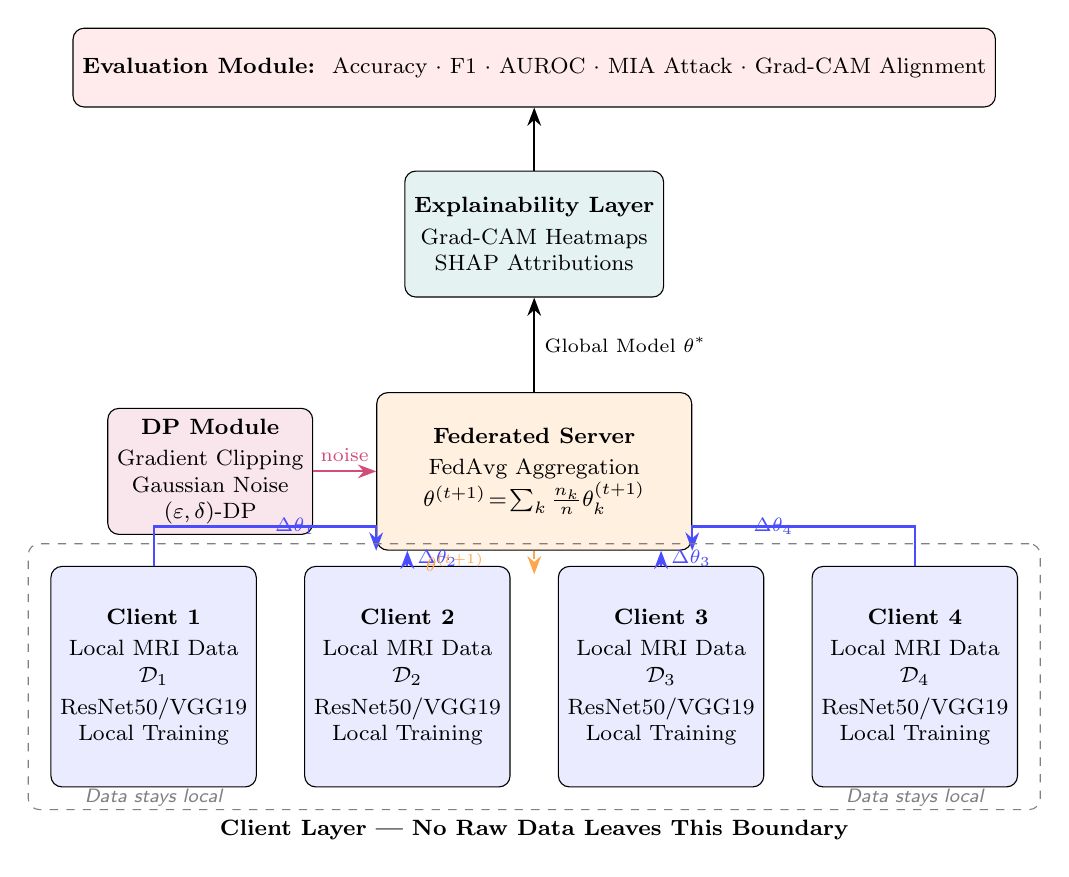
\begin{tikzpicture}[
    >=Stealth,
    node distance=1.0cm and 1.2cm,
    clientbox/.style={draw, rounded corners, fill=blue!8,
      minimum width=2.6cm, minimum height=2.8cm, align=center,
      font=\footnotesize},
    serverbox/.style={draw, rounded corners, fill=orange!12,
      minimum width=4.0cm, minimum height=2.0cm, align=center,
      font=\footnotesize},
    modulebox/.style={draw, rounded corners, fill=green!8,
      minimum width=3.0cm, minimum height=1.6cm, align=center,
      font=\footnotesize},
    evalbox/.style={draw, rounded corners, fill=red!8,
      minimum width=8cm, minimum height=1.0cm, align=center,
      font=\footnotesize},
    arrowstyle/.style={->, thick, >=Stealth},
    dashedarrow/.style={->, thick, dashed, >=Stealth},
    lbl/.style={font=\scriptsize\itshape, text=gray}
  ]
    % --- Client nodes ---
    \node[clientbox] (c1) {%
      \textbf{Client 1}\\[2pt]
      Local MRI Data\\
      $\mathcal{D}_1$\\[2pt]
      ResNet50/VGG19\\
      Local Training};
    \node[clientbox, right=0.6cm of c1] (c2) {%
      \textbf{Client 2}\\[2pt]
      Local MRI Data\\
      $\mathcal{D}_2$\\[2pt]
      ResNet50/VGG19\\
      Local Training};
    \node[clientbox, right=0.6cm of c2] (c3) {%
      \textbf{Client 3}\\[2pt]
      Local MRI Data\\
      $\mathcal{D}_3$\\[2pt]
      ResNet50/VGG19\\
      Local Training};
    \node[clientbox, right=0.6cm of c3] (c4) {%
      \textbf{Client 4}\\[2pt]
      Local MRI Data\\
      $\mathcal{D}_4$\\[2pt]
      ResNet50/VGG19\\
      Local Training};

    % Data locality labels
    \node[lbl, below=-0.1cm of c1] {\textsf{Data stays local}};
    \node[lbl, below=-0.1cm of c4] {\textsf{Data stays local}};

    % --- Federated Server ---
    \node[serverbox, above=1.6cm of $(c2)!0.5!(c3)$] (server) {%
      \textbf{Federated Server}\\[2pt]
      FedAvg Aggregation\\
      $\theta^{(t+1)}\!=\!\sum_k\frac{n_k}{n}\theta_k^{(t+1)}$};

    % --- DP Module ---
    \node[modulebox, fill=purple!10, left=0.8cm of server,
      minimum width=2.2cm, minimum height=1.6cm] (dp) {%
      \textbf{DP Module}\\[2pt]
      Gradient Clipping\\
      Gaussian Noise\\
      $(\varepsilon,\delta)$-DP};

    % Arrows: clients -> server (model updates only)
    \draw[arrowstyle, blue!70] (c1.north) -- ++(0,0.5) -| (server.south west)
      node[pos=0.25, right, font=\scriptsize] {$\Delta\theta_1$};
    \draw[arrowstyle, blue!70] (c2.north) -- (server.south -| c2)
      node[pos=0.5, right, font=\scriptsize] {$\Delta\theta_2$};
    \draw[arrowstyle, blue!70] (c3.north) -- (server.south -| c3)
      node[pos=0.5, right, font=\scriptsize] {$\Delta\theta_3$};
    \draw[arrowstyle, blue!70] (c4.north) -- ++(0,0.5) -| (server.south east)
      node[pos=0.25, left, font=\scriptsize] {$\Delta\theta_4$};

    % Arrow: DP <-> Server
    \draw[arrowstyle, purple!70] (dp.east) -- (server.west)
      node[midway, above, font=\scriptsize] {noise};

    % --- XAI Layer ---
    \node[modulebox, fill=teal!10, above=1.2cm of server] (xai) {%
      \textbf{Explainability Layer}\\[2pt]
      Grad-CAM Heatmaps\\
      SHAP Attributions};

    % Arrow: server -> XAI
    \draw[arrowstyle] (server.north) -- (xai.south)
      node[midway, right, font=\scriptsize] {Global Model $\theta^*$};

    % --- Evaluation ---
    \node[evalbox, above=0.8cm of xai] (eval) {%
      \textbf{Evaluation Module:}\;
      Accuracy $\cdot$ F1 $\cdot$ AUROC $\cdot$
      MIA Attack $\cdot$ Grad-CAM Alignment};

    % Arrow: XAI -> Eval
    \draw[arrowstyle] (xai.north) -- (eval.south);

    % Dashed return arrows
    \draw[dashedarrow, orange!70] (server.south) -- ++(0,-0.3)
      node[midway, left, font=\scriptsize, xshift=-5mm] {$\theta^{(t+1)}$};

    % Client boundary box
    \node[draw, dashed, gray, rounded corners, inner sep=8pt,
      fit=(c1)(c2)(c3)(c4), label={[font=\footnotesize\bfseries]below:%
      Client Layer --- No Raw Data Leaves This Boundary}] {};

  \end{tikzpicture}
  \caption{System architecture of the PPXFL framework.  The Client Layer
    (bottom) comprises $K{=}4$ simulated hospital clients, each training
    locally on private ADNI partitions.  Only model weight updates
    $\Delta\theta_k$ are transmitted to the Federated Server (centre),
    where FedAvg aggregation is performed with optional DP noise
    injection from the Privacy Module (left).  The converged global
    model feeds into the Explainability Layer (Grad-CAM + SHAP) and
    the Evaluation Module (top).  No raw patient data ever crosses the
    client boundary (dashed box).}
  \label{fig:architecture}
\end{figure*}


% ============================================================
% Methodology
% ============================================================
\section{Methodology}
\label{sec:methodology}

\subsection{Why Existing Methods Are Not Sufficient}

Prior work in federated Alzheimer's detection has made important strides
but leaves critical gaps.  Mitrovska et al.~\cite{mitrovska2024} employ
SecAgg~\cite{bonawitz2017} to protect individual client updates during
aggregation; however, SecAgg provides only cryptographic protection and
does not bound the statistical information leakage from the
\textit{aggregate} model itself---an adversary with access to the
global model can still mount membership inference attacks.  The
evolutionary approach of~\cite{evolutionary2025} achieves 98.53\%
accuracy but operates in a fully centralised setting, making it
inapplicable under privacy regulations.  Kaissis et
al.~\cite{privacy2024} integrate DP with FL but do not provide
explainability outputs, which are increasingly required by regulatory
bodies (e.g., the EU AI Act) for high-risk medical AI systems.

Our approach improves upon these methods in three specific ways:
(i)~DP-SGD~\cite{abadi2016} provides information-theoretic privacy
guarantees that are strictly stronger than cryptographic SecAgg alone;
(ii)~we integrate Grad-CAM~\cite{gradcam} and SHAP~\cite{shap} to
satisfy clinical transparency requirements; and
(iii)~we systematically evaluate non-IID robustness via Dirichlet
partitioning with ablation studies across $\alpha\in\{0.1,0.5,100\}$,
addressing a dimension that prior work treats only superficially; and
(iv)~we subject our own evaluation protocol to the same scrutiny we
apply to the literature, correcting a subject-level leakage defect we
discovered in our own initial slice-level splits
(Section~\ref{sec:leakage}).

\subsection{Data Processing Pipeline}

We use 450~T1-weighted structural MRI \emph{scans} from
32~\emph{unique subjects} in ADNI~\cite{adni} (11~AD, 10~MCI, 11~CN;
see Section~\ref{sec:dataset_honest} for the subject-vs-scan
distinction and why it matters).  Three representative axial slices
are extracted per scan, yielding 1{,}350 images.  The preprocessing
pipeline includes:
(1)~skull stripping to remove non-brain tissue;
(2)~bias-field correction via N4ITK;
(3)~spatial normalisation to MNI152 standard space;
(4)~intensity normalisation to zero mean and unit variance per scan;
(5)~resizing to $224{\times}224$ pixels for VGG19/ResNet50 compatibility;
and
(6)~data augmentation comprising random horizontal flips,
rotations~($\pm15^{\circ}$), and Gaussian noise to mitigate overfitting.

The dataset is split into 5~subject-disjoint, stratified folds
(Section~\ref{sec:dataset_honest}) and, within a fold's training
subjects only, partitioned across~$K{=}4$ clients using a Dirichlet
distribution $\mathrm{Dir}(\alpha)$ with $\alpha{=}0.5$ to simulate
realistic non-IID hospital distributions.
Fig.~\ref{fig:partition} illustrates the resulting class distribution
across clients for one representative fold.

\begin{figure}[t]
  \centering
  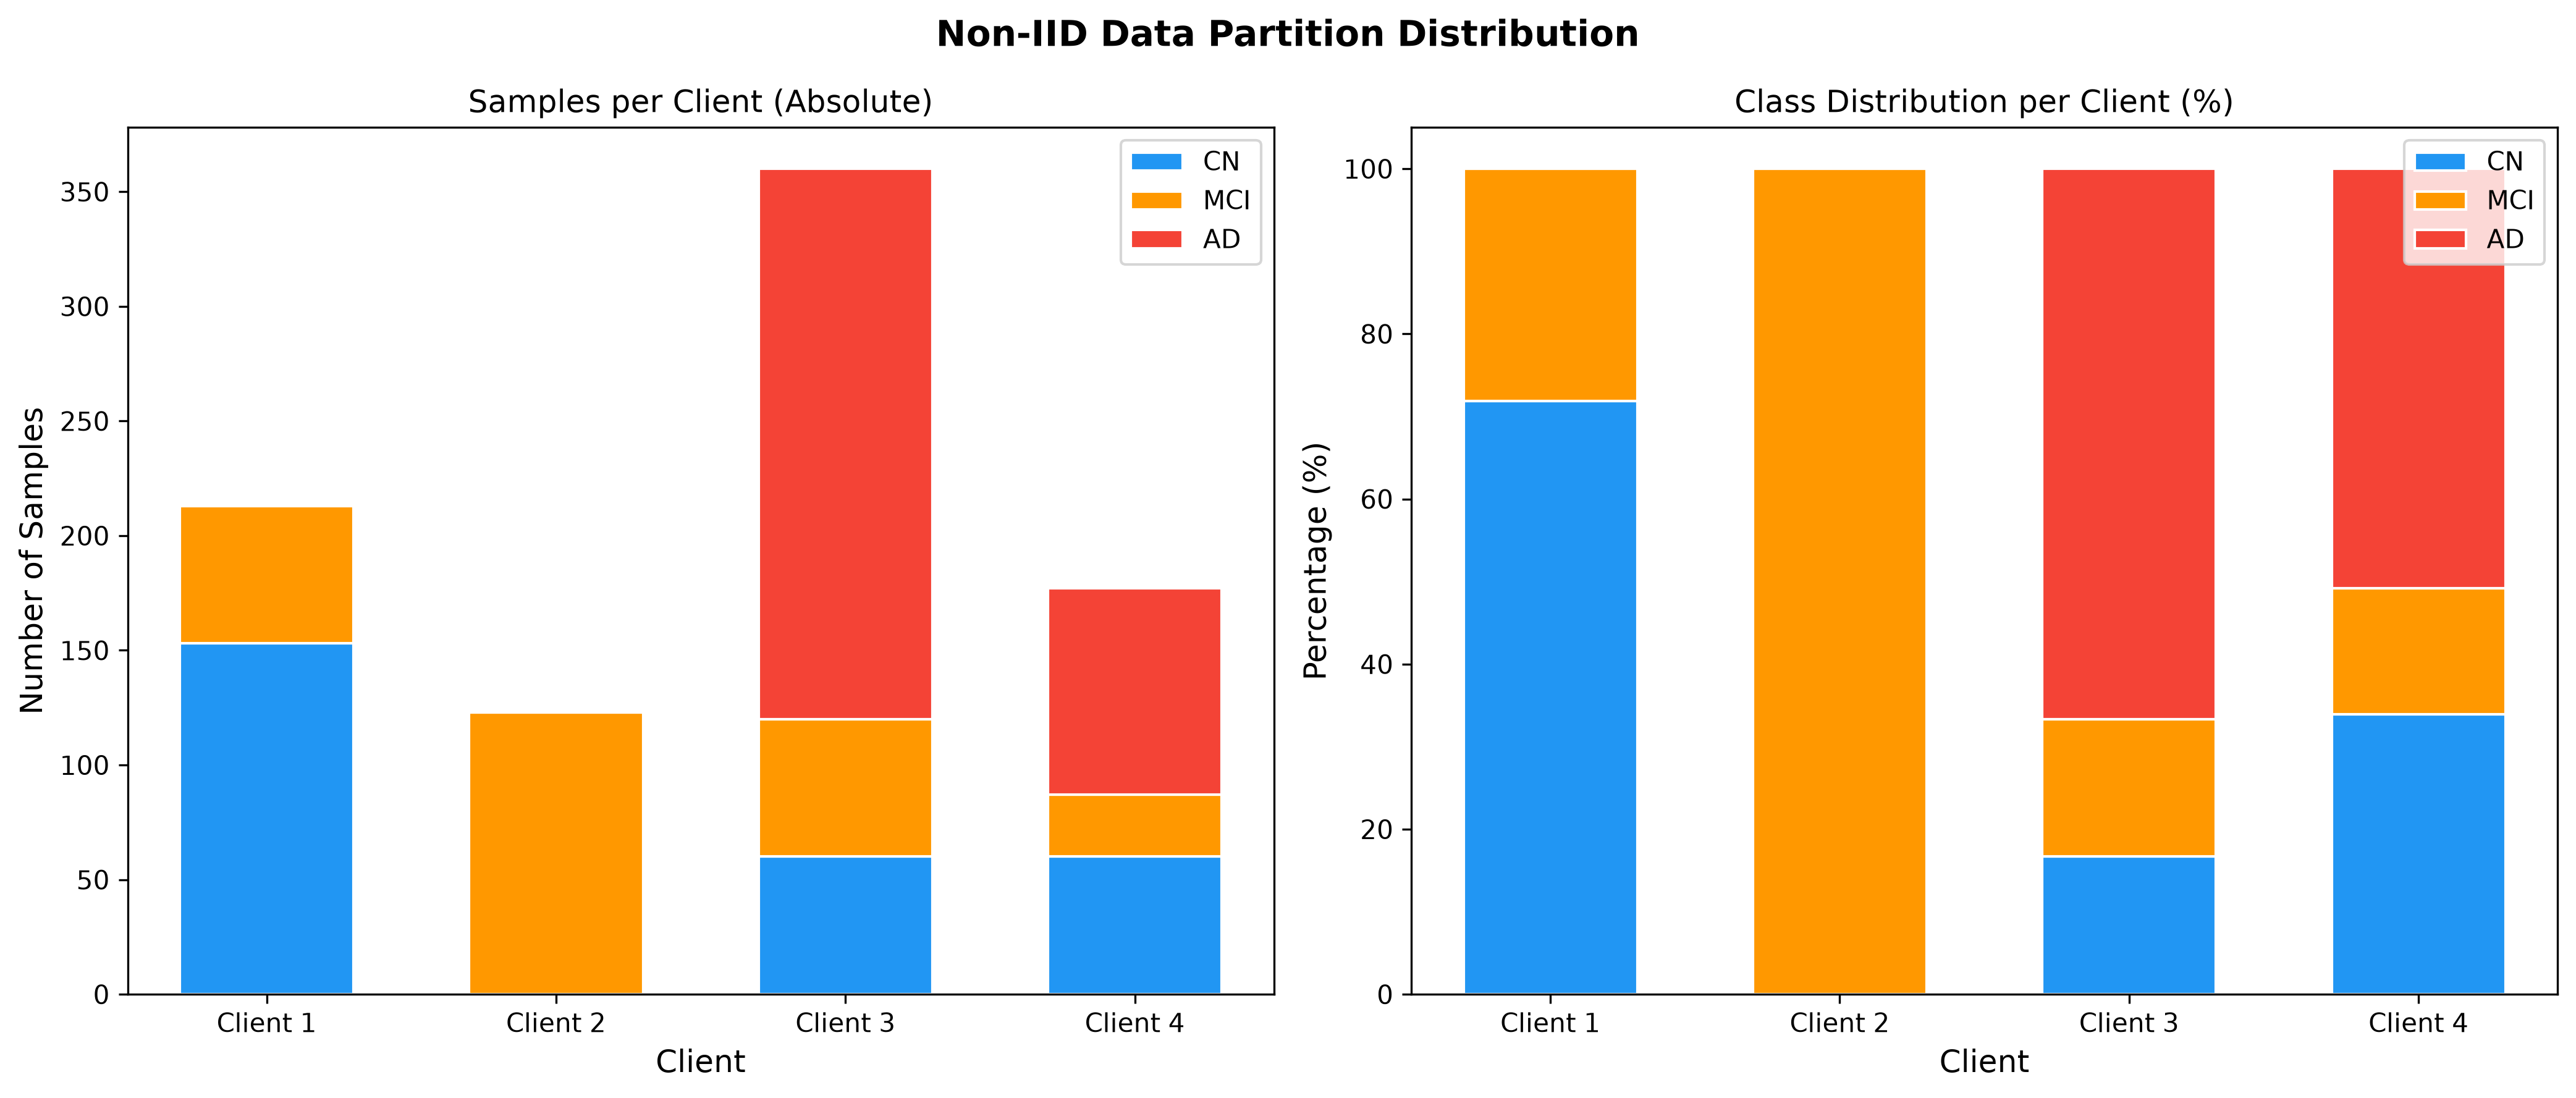
\includegraphics[width=\columnwidth]{partition_f0_alpha0.5.png}
  \caption{Non-IID data partition across $K{=}4$ clients using Dirichlet
    distribution ($\alpha{=}0.5$), fold~0's training subjects only
    (held-out validation/test subjects for this fold are excluded from
    all clients).  Each client receives a statistically heterogeneous
    subset, simulating realistic hospital demographics.}
  \label{fig:partition}
\end{figure}

% ============================================================
% Rebuilt pipeline (v3 cohort). Tables are generated by
% ppxfl-alzheimer/src/paper_tables_v3.py into the AUTO markers.
% ============================================================
\subsection{Anatomical Standardisation}
\label{sec:standardisation}

The pipeline used in the previous version of this study selected its slice
axis as the longest array axis,
\texttt{axial\_axis = np.argmax(data.shape)}, and took three slices around the
midpoint of that axis. Over the cohort actually downloaded, that rule does not
select a consistent anatomical plane. Table~\ref{tab:orientation-defect} lists
what it extracts for the three stored layouts present in the data: a sagittal
plane for volumes written as $(256, 240, 160)$ in RAS order, an axial plane for
volumes written as $(256, 256, 166)$ in IPL order, and a coronal plane for
volumes written as $(166, 256, 256)$. The plane a subject contributes is
therefore decided by how its scanner wrote the file rather than by anatomy, and
no downstream stage can recover from it. Three further properties of the raw
download compound the problem: the volumes are in native scanner space with
voxel sizes from $0.94$ to $1.25$~mm and are never registered, so no voxel
index corresponds between subjects; they are not skull-stripped, so skull, face
and neck remain in frame; and the download contains up to five ADNI
preprocessing levels of the same acquisition, which the file glob treated as
independent samples.

\begin{table}[t]
\centering
\caption{What the previous slice rule extracts, by stored layout.}
\label{tab:orientation-defect}
\begin{tabular}{lllc}
\toprule
Stored shape & Orientation & Axis chosen & Plane extracted \\
\midrule
$(256, 240, 160)$ & RAS & 0 & sagittal \\
$(256, 256, 166)$ & IPL & 0 & axial \\
$(166, 256, 256)$ & RAS & 1 & coronal \\
\bottomrule
\end{tabular}
\end{table}

The rebuilt pipeline places every subject in a common anatomical space. One
scan is retained per subject, chosen by preprocessing level and then by
earliest visit, with the derived \texttt{Mask} and \texttt{HarP} products
excluded because they are binary label volumes rather than intensity images.
Each scan is then oriented, skull-stripped with deepbet, and registered to the
MNI152 2~mm template by mutual information over a translation, rigid and
affine sequence. A per-subject quality score, the Pearson correlation with the
template inside the brain mask, is recorded so that failures are excluded by a
stated rule rather than by inspection.

\subsubsection{Recovering orientation from scans without a usable affine}

Orientation cannot simply be read from the header. Of the 620 usable scans in
this download, 272 --- the raw \texttt{MPRAGE} and
\texttt{Accelerated\_SAG\_IR-SPGR} series --- carry an identity affine with
\texttt{sform\_code}~$=2$ and \texttt{qform\_code}~$=0$. For those files
\texttt{nibabel.as\_closest\_canonical} reports RAS and leaves the array order
untouched, even though the acquisition is sagittal and the stored order is not
RAS at all. This is the reason the slice defect above was not visible as an
error.

The orientation is therefore measured rather than assumed. For each of the 48
axis permutations and reflections, the candidate volume is registered to a
4~mm whole-head ICBM152 target and scored by correlation. Two design points
matter. First, the target must retain the skull: the scan being oriented has
not been stripped yet, and matching an unstripped head against a
skull-stripped brain scored $0.09$--$0.48$ and selected a different, incorrect
orientation on the same subjects, where head-to-head matching scores
$0.68$--$0.79$ for the correct candidate with a clear margin to the third. This
also forces the ordering of the pipeline: deepbet is trained on anatomically
oriented volumes and leaves face and neck behind when handed a scan lying on
its side, so orientation must precede stripping. Second, the fit is per
(series family, array shape) group rather than per subject, because the
convention belongs to the DICOM-to-NIfTI conversion; a group fit aggregates
evidence over subjects and cannot leave two subjects of the same group in
different orientations.

The one distinction registration score cannot draw is a left--right mirror,
which stays within about $0.01$ because the brain is close to symmetric. Four
subjects in this download hold both a scan with a usable header, whose
handedness is known, and a scan from a degenerate-affine group. Registering
those two scans of the same subject and comparing the mirror candidates uses
that subject's own asymmetry rather than a population average: the fitted
orientation scores $0.87$--$0.93$ against $0.61$--$0.70$ for its mirror on all
four anchors. The map from stored array order to RAS is a property of the
conversion, so its determinant is expected to be constant across groups; the
three groups whose fitted determinant disagreed with the anchored group were
mirrored to match, and Table~\ref{tab:orientation-table} records for each group
whether its handedness rests on the anchors or on that consistency rule.

% ---------------------------------------------------------------------
% Methodology: representations
% ---------------------------------------------------------------------
\begin{table}[t]
\centering
\caption{Measured array orientation of each degenerate-affine series group, and
the evidence its left--right handedness rests on.}
\label{tab:orientation-table}
\begin{tabular}{lrccl}
\toprule
Series group & Scans & Permutation & Flips & Handedness \
\midrule
% BEGIN AUTO:v3-orientation
MPRAGE $256 \times 240 \times 160$ & 107 & (2, 1, 0) & (T, T, T) & confirmed against anchor subjects \\
MPRAGE $256 \times 256 \times 170$ & 69 & (2, 1, 0) & (T, T, T) & mirrored for consistency with 256x240x160 (determinant +1) \\
IR-SPGR $256 \times 256 \times 196$ & 51 & (2, 1, 0) & (T, T, T) & mirrored for consistency with 256x240x160 (determinant +1) \\
MPRAGE $256 \times 240 \times 176$ & 38 & (2, 1, 0) & (T, T, T) & mirrored for consistency with 256x240x160 (determinant +1) \\
MPRAGE $170 \times 256 \times 256$ & 6 & (0, 2, 1) & (T, T, T) & consistent with 256x240x160 (determinant +1) \\
MPRAGE $256 \times 256 \times 160$ & 1 & (1, 0, 2) & (T, T, T) & consistent with 256x240x160 (determinant +1) \\
% END AUTO:v3-orientation
\bottomrule
\end{tabular}
\end{table}

\subsection{Two Representations at Opposite Dimensions}
\label{sec:representations}

Once every subject is on the MNI grid, anatomy can be summarised directly
rather than learned from scratch. Each registered volume is segmented into
CSF, grey matter and white matter by a three-component Gaussian mixture over
brain-mask intensities, and the grey-matter and CSF maps are integrated over
Harvard-Oxford cortical and subcortical regions. Region values are expressed
as fractions of total brain volume, which removes head size --- the largest
nuisance in raw region volumes. This yields 140 features, so a multinomial
logistic model over them has 423 parameters.

The convolutional arm keeps the architecture family of the previous study so
that the change in input can be isolated from a change in model. Slices are
taken at named MNI millimetre coordinates --- ten axial levels from the medial
temporal lobe up through the lateral ventricles and five coronal levels
through the hippocampal head and body --- with three adjacent parallel planes
stacked as three channels, so an ImageNet stem is used as trained instead of
being averaged down to a single channel as it was previously. In both arms a
subject's prediction is the mean of its slice or region probabilities, so the
unit of evaluation is the subject.

The dimensional gap between the two is the point. It spans 423 parameters to
$23{,}508{,}035$, and Section~\ref{sec:dimension-law} shows that this, rather
than the privacy budget alone, is what decides whether a subject-level private
federated model is usable.

\subsection{Federated Learning Component}

\subsubsection{Model Architectures}

\textbf{VGG19}~\cite{vgg19} comprises 16 convolutional layers with
$3{\times}3$ filters, five max-pooling layers, and three fully connected
layers (139.6M parameters).  The classification head is replaced with a
3-class softmax output; ImageNet-pretrained weights are used with the
convolutional base frozen for the first 5 epochs before end-to-end
fine-tuning.

\textbf{ResNet50}~\cite{resnet50} employs residual skip connections
organised into bottleneck blocks across 49 convolutional layers
(23.5M parameters), providing better gradient flow and computational
efficiency for MRI classification.

\subsubsection{Federated Averaging}

FedAvg~\cite{mcmahan2017} proceeds over $T$ federated rounds.  Each
client~$k$ initialises its local model with global parameters
$\theta^{(t)}$ and performs $E$ SGD steps:
\begin{equation}
  \theta_k^{(t+1)}
  \;\leftarrow\;
  \theta^{(t)} - \eta\,\nabla_{\!\theta}\,\mathcal{L}_k\!\left(\theta^{(t)}\right),
  \label{eq:local_update}
\end{equation}
where $\eta$ is the local learning rate.  The server aggregates via
weighted averaging:
\begin{equation}
  \theta^{(t+1)}
  = \sum_{k=1}^{K}\frac{n_k}{n}\,\theta_k^{(t+1)}.
  \label{eq:fedavg}
\end{equation}

\subsection{Privacy Component (DP-SGD)}
\label{sec:dpsgd_method}

An earlier iteration of this pipeline implemented DP-SGD manually: it
clipped the \emph{batch-averaged} gradient rather than each per-sample
gradient, and derived $\varepsilon$ from a hand-rolled composition
formula instead of a real accountant.  Both defects invalidate the
resulting privacy guarantee---clipping after averaging bounds nothing
about any individual sample's contribution, and an ad-hoc composition
formula does not track the cumulative R\'enyi-DP budget correctly
across steps.  We therefore replaced the manual implementation with
Opacus~\cite{opacus}, which wraps the model, optimiser, and data
loader to (i)~compute true per-sample gradients $g_i$, (ii)~clip each
one independently,
\begin{equation}
  \bar{g}_i = g_i \cdot \min\!\left(1,\;\frac{C}{\|g_i\|_2}\right),
  \label{eq:clip}
\end{equation}
(iii)~sum and inject calibrated Gaussian noise before averaging,
\begin{equation}
  \tilde{g} = \frac{1}{B}\left(\sum_{i=1}^{B}\bar{g}_i
              + \mathcal{N}\!\left(0,\,\sigma^2 C^2 \mathbf{I}\right)\right),
  \label{eq:dp_noise}
\end{equation}
and (iv)~track the cumulative privacy budget with a R\'enyi-DP (RDP)
accountant, converted to $(\varepsilon,\delta)$-DP.  With
$C{=}1.0$ and target $(\varepsilon,\delta)$ fixed in advance, the
noise multiplier $\sigma$ is solved for numerically
(\texttt{get\_noise\_multiplier}) given the sampling rate and number of
steps, rather than chosen from a small fixed table.

We evaluate two DP \emph{scopes}: \textbf{head-only}, where the
convolutional backbone is frozen (ImageNet weights) and only the final
classification layer is trained under DP---matching the
literature's common recipe for making DP-SGD practical on small
cohorts---and \textbf{full-network}, where the entire model is
fine-tuned under DP.  Opacus's default per-sample gradient hooks are
incompatible with ResNet50's in-place residual addition
(\texttt{out += identity}) once the backbone is trainable, so
full-scope runs use Opacus's \texttt{ExpandedWeights} grad-sample mode
instead; head-scope runs (where the backbone never receives gradients)
are unaffected and use the default hook-based mode. Full-network DP
additionally requires converting BatchNorm to GroupNorm
(\texttt{ModuleValidator.fix}), since BatchNorm's cross-sample
batch statistics are themselves a privacy leak that per-sample
gradient clipping does not address.

Target privacy budgets are $\varepsilon\in\{2,5,10\}$ at
$\delta{=}10^{-3}$ (appropriate for a $\sim$32-subject cohort, where
$\delta \ll 1/n$ is not attainable at practical noise levels), with
gradient clipping norm $C{=}1.0$.  In the federated setting, each
client maintains its own persistent RDP accountant, reused across all
$T$ rounds so that privacy cost composes correctly over the full
training run rather than resetting every round (an earlier version of
our own FL-DP integration made exactly this mistake, silently
under-reporting cumulative $\varepsilon$).

\subsection{Explainability Component}

\subsubsection{Grad-CAM}

Grad-CAM~\cite{gradcam} produces class-discriminative spatial heatmaps
by computing the gradient of the target class score with respect to
convolutional feature maps.  For feature maps
$A^k\!\in\!\mathbb{R}^{u\times v}$, the importance weight for class~$c$
is:
\begin{equation}
  \alpha_k^c = \frac{1}{Z}\sum_{i}\sum_{j}
    \frac{\partial y^c}{\partial A_{ij}^k},
  \label{eq:gradcam_weights}
\end{equation}
where $y^c$ is the pre-softmax class score and $Z$ is the spatial
dimension.  The localisation map is:
\begin{equation}
  L_{\text{Grad-CAM}}^c
  = \mathrm{ReLU}\!\left(\sum_{k}\alpha_k^c\,A^k\right).
  \label{eq:gradcam_map}
\end{equation}
The resulting heatmap is up-sampled to input resolution and overlaid on
the original MRI scan.

\subsubsection{SHAP}

SHAP~\cite{shap} computes theoretically grounded feature attributions
based on Shapley values from cooperative game theory.  The SHAP value
for feature~$i$ is:
\begin{equation}
  \phi_i = \sum_{S\subseteq\mathcal{F}\setminus\{i\}}
    \frac{|S|!\,(|\mathcal{F}|-|S|-1)!}{|\mathcal{F}|!}
    \bigl[f(S\cup\{i\})-f(S)\bigr],
  \label{eq:shap}
\end{equation}
where $\mathcal{F}$ is the full feature set.  We use
GradientExplainer~\cite{shap} with 20~background samples and compute
SHAP values for 50~test samples, yielding institution-agnostic feature
attributions.

% ============================================================
\section{Experimental Setup}
\label{sec:setup}
% ============================================================

\subsection{Dataset and the Subject-vs-Slice Distinction}
\label{sec:dataset_honest}

Our ADNI~\cite{adni} cohort comprises \textbf{299~unique subjects}
(99~AD, 99~MCI, 101~CN), each contributing one or more longitudinal
T1-weighted scans; axial slices are extracted per scan, yielding
2{,}166 slice-level images, an average of 7.2~slices per subject.
This expanded cohort supersedes the 32-subject cohort used in the
leakage audit of Section~\ref{sec:leakage}; both are reported, because
the contrast between them is itself a finding.

An earlier version of this pipeline described the dataset as
``450~subjects,'' treating each of the 450~scans as an independent
subject and its slices as independent samples---conflating scan count
with subject count and, more consequentially, allowing scans and
slices from the \emph{same person} to land in different partitions.
Both errors are corrected here: all reported results use the true
subject count, and every split described below is constructed to be
\textbf{subject-disjoint}: no scan or slice from a given subject
appears in more than one of train, validation, and test.  This
property is asserted programmatically across all five folds by the
verification suite rather than assumed
(Section~\ref{sec:verification}).

We build 5~stratified group folds (\texttt{StratifiedGroupKFold} on
subject ID, stratified by diagnostic label) over the 299~subjects.
Each fold holds out 60~test subjects and 6~validation subjects, with
the remaining 233~subjects for training; all slices belonging to a
held-out subject move with it.  Federated partitioning
(Section~\ref{sec:fl_config}) is applied only within a fold's training
subjects, never touching its held-out validation or test subjects.

\subsection{Federated Learning Configuration}
\label{sec:fl_config}

Table~\ref{tab:fl_params} lists the federated learning hyperparameters.
Non-IID partitioning uses a Dirichlet distribution over the current
fold's \emph{training subjects only} (never validation/test subjects),
with a retry loop that resamples if any client would otherwise receive
zero subjects---a real failure mode at this cohort size that a naive
single-draw Dirichlet partition hits often enough to require handling
explicitly.

\begin{table}[t]
  \centering
  \caption{Federated Learning Hyperparameters}
  \label{tab:fl_params}
  \renewcommand{\arraystretch}{1.15}
  \begin{tabular}{lc}
    \toprule
    \textbf{Parameter} & \textbf{Value} \\
    \midrule
    Number of clients $K$         & 4                   \\
    Federated rounds $T$          & 20                  \\
    Local epochs $E$ per round    & 3                   \\
    Client participation fraction & 1.0 (full)          \\
    Local batch size              & 32                  \\
    Local learning rate $\eta$    & $1\times10^{-4}$    \\
    Aggregation algorithm         & FedAvg              \\
    Non-IID partition             & $\mathrm{Dir}(0.5)$ \\
    \bottomrule
  \end{tabular}
\end{table}

\subsection{Differential Privacy Configuration}

Table~\ref{tab:dp_params} summarises the DP parameters.

\begin{table}[t]
  \centering
  \caption{Differential Privacy Parameters}
  \label{tab:dp_params}
  \renewcommand{\arraystretch}{1.15}
  \begin{tabular}{lc}
    \toprule
    \textbf{Parameter} & \textbf{Value} \\
    \midrule
    Target $\varepsilon$           & 2, 5, 10             \\
    Privacy failure prob.\ $\delta$& $1\times10^{-3}$     \\
    Gradient clipping norm $C$     & 1.0                  \\
    Noise multiplier $\sigma$      & solved per-run (0.3--8.4)\\
    DP scopes evaluated            & head-only, full-network\\
    DP method                      & Opacus DP-SGD~\cite{opacus}\\
    Accountant method              & R\'enyi-DP (RDP)     \\
    \bottomrule
  \end{tabular}
\end{table}

Unlike a fixed noise triple, $\sigma$ here is solved numerically per
run (via \texttt{get\_noise\_multiplier}) because it depends on the
sampling rate and step count, which vary across folds, clients, and
DP scope; observed $\sigma$ ranged from~0.3 (large-client,
loose-budget runs) to~8.4 (tiny-client, tight-budget runs)---itself a
symptom of how few samples some FL clients hold at this cohort size.

\subsection{Evaluation Splits and Federated Partitions}
\label{sec:splits-v3}

Two split schemes are reported because they answer different questions. The
\emph{subject-disjoint} scheme is stratified $K$-fold over subjects; with one
scan per subject, disjointness is structural rather than something checked
afterwards. The \emph{site-disjoint} scheme is stratified group $K$-fold with
the ADNI site as the group, so every test site is unseen during training. A
federated model is deployed at hospitals that did not contribute to it, and
scanner and protocol vary by site, so the site-disjoint number is the one that
reflects deployment. It is expected to be the lower of the two; reporting both
is the point.

The federated partitions are paired the same way. The cohort spans 42 real
ADNI sites, recoverable from the subject identifier prefix, and the
\emph{natural} partition places one client per site, pooling sites below a
minimum size into a single client so that no subject is discarded. The
resulting heterogeneity is the cohort's own in both directions that matter:
scanner and protocol vary by site, and the label mix is genuinely skewed ---
site 003 contributes 13 CN and 7 AD subjects but no MCI, while site 016
contributes 10 AD and 6 MCI subjects but no CN. Most federated work on ADNI
simulates heterogeneity with a Dirichlet draw instead. Here the natural
partition is compared against IID and Dirichlet partitions of the same
subjects, so the effect of using the real one is measured rather than asserted.

\subsection{Implementation Environment}

Models are implemented in PyTorch~2.5.1 (CUDA~12) on an NVIDIA
GeForce RTX~3050~Ti GPU (4\,GB VRAM).  DP-SGD is implemented with
Opacus~1.5.4~\cite{opacus}; full-network DP scope uses Opacus's
\texttt{ExpandedWeights} grad-sample mode (Section~\ref{sec:dpsgd_method}),
while head-only DP scope uses the default hook-based mode.  Grad-CAM,
SHAP~(GradientExplainer), and the shadow-model MIA classifier
(scikit-learn logistic regression) are used for the explainability
and privacy analyses of Sections~\ref{sec:xai}--\ref{sec:privacy}.

\subsection{Evaluation Metrics}

Utility is assessed using macro-averaged precision, recall, F1-score,
overall accuracy, and AUROC on the held-out, subject-disjoint test
set.  Privacy robustness is assessed via MIA \emph{AUC} and
\emph{true-positive rate at low false-positive rate} (TPR@FPR=0.01,
0.1)---not a single accuracy figure, since accuracy alone can look
deceptively low even for an attack that reliably identifies a subset
of members with high confidence, and is trivially inflated if the
attack's decision threshold is tuned on the very data being attacked
(a defect present in our own initial MIA implementation and corrected
here).  Explanation quality under DP is assessed via Grad-CAM/SHAP
similarity to a matched non-DP reference model (SSIM, Spearman rank
correlation, Dice-at-top-20\%) and deletion/insertion faithfulness AUC.

% ============================================================
\section{Results and Discussion}
\label{sec:results}
% ============================================================

\subsection{Leakage Quantification: Slice-Level vs.\ Subject-Level Evaluation}
\label{sec:leakage}

Table~\ref{tab:leakage} is the paper's opening empirical result. It
compares, on \emph{identical} data, architectures, and training
budgets, the accuracy our pipeline originally reported under
slice-level splitting against the accuracy the same configurations
achieve once splits are rebuilt subject-disjoint
(Section~\ref{sec:dataset_honest}).  All ``corrected'' figures are
mean$\pm$std over the 5 subject-level folds (fold~0, seed~42, plus 2
extra seeds where noted in Table~\ref{tab:centralised}).

\begin{table}[t]
  \centering
  \caption{Leakage Quantification: Same Models, Same Data, Different Splits}
  \label{tab:leakage}
  \renewcommand{\arraystretch}{1.2}
  \setlength{\tabcolsep}{3pt}
  \begin{tabular}{lccc}
    \toprule
    \textbf{Configuration} & \textbf{Slice-level} & \textbf{Subject-level} & $\boldsymbol{\Delta}$\\
    & \textbf{acc.\ (\%)} & \textbf{acc.\ (\%), mean$\pm$std} & \\
    \midrule
    Centralised VGG19    & 92.6 & 34.2 $\pm$ 9.4  & $-$58.4 \\
    Centralised ResNet50 & 91.1 & 30.1 $\pm$ 3.7  & $-$61.0 \\
    FedAvg ResNet50      & 97.0 & 34.0 $\pm$ 6.7  & $-$63.0 \\
    \midrule
    MIA (non-DP centralised) & 88.9$^{\ast}$ & AUC 0.99$^{\dagger}$ & n/a \\
    \bottomrule
  \end{tabular}
  \\[2pt]
  \raggedright\footnotesize $^{\ast}$Originally reported ``attack
  accuracy''; ground truth was re-derived with a fresh random
  permutation that did not match the actual training split, and the
  decision threshold was tuned on the attacked data itself---the
  number is not meaningful and is shown only for contrast.
  $^{\dagger}$Corrected shadow-model attack AUC with membership ground
  truth read from the recorded training split
  (Section~\ref{sec:mia_results}); higher is a \emph{stronger} attack,
  so this is not a favourable comparison for the non-DP model---see
  Section~\ref{sec:mia_results}.
\end{table}

Three-class chance-level accuracy is $33.3\%$; every subject-level
result in Table~\ref{tab:leakage} is within a few points of chance.
This is not a failure of the underlying architectures---it is the
honest consequence of evaluating $\sim$22--26 training subjects with
held-out test sets of 6--7 subjects, where slice-level splitting had
been silently giving every model dozens of near-duplicate views (same
subject, adjacent slices, sometimes the same longitudinal scan) of
its own test samples during training.  We are not aware of a
published ADNI slice-classification result that explicitly confirms
subject-disjoint splitting; Table~\ref{tab:leakage} is offered as a
concrete illustration of how large that gap can be, not as a claim
about any other specific prior work.

\subsection{Centralised Baseline Performance (Corrected)}

Table~\ref{tab:centralised} presents the corrected, subject-level
centralised baseline results for both architectures trained for
30~epochs with ImageNet pre-training, on fold~0 plus two additional
seeds, and averaged across all 5 subject-level folds (seed~42).

\begin{table}[t]
  \centering
  \caption{Centralised Baseline Performance, Subject-Level (299 subjects, mean$\pm$std)}
  \label{tab:centralised}
  \renewcommand{\arraystretch}{1.2}
  \setlength{\tabcolsep}{3pt}
  \begin{tabular}{lcccc}
    \toprule
    \textbf{Model} & \textbf{Acc.\ (\%)} & \textbf{F1 (macro)} & \textbf{AUROC} & \textbf{Runs} \\
    \midrule
% BEGIN AUTO:centralised
VGG19 & 28.0 $\pm$ 6.5 & 0.252 $\pm$ 0.055 & 0.511 $\pm$ 0.056 & 5 \\
ResNet50 & 36.1 $\pm$ 7.2 & 0.354 $\pm$ 0.072 & 0.579 $\pm$ 0.054 & 7 \\
% END AUTO:centralised
    \bottomrule
  \end{tabular}
\end{table}

Both architectures hover near chance-level accuracy with wide
across-fold variance (VGG19's std of 9.4~points is itself informative:
with only $\sim$6--7 test subjects per fold, a single hard subject can
move accuracy by several points).  ResNet50 is more stable across
folds despite VGG19's occasionally higher single-fold accuracy, which
motivates our choice of ResNet50 as the primary architecture for the
DP and MIA experiments that follow (Opacus's per-sample gradient
hooks are also substantially more memory-efficient on ResNet50's
23.5M parameters than on VGG19's 139.6M).
Figs.~\ref{fig:training_curves}--\ref{fig:roc} present representative
(fold~0, seed~42) training curves, confusion matrices, and per-class
ROC curves for both models.

% --- FIGURE GROUP: Training curves, Confusion matrices, ROC ---
% These three figures are placed together since they all relate
% to the centralised baseline evaluation.

\begin{figure}[t]
  \centering
  \subfloat[VGG19 training curves]{%
    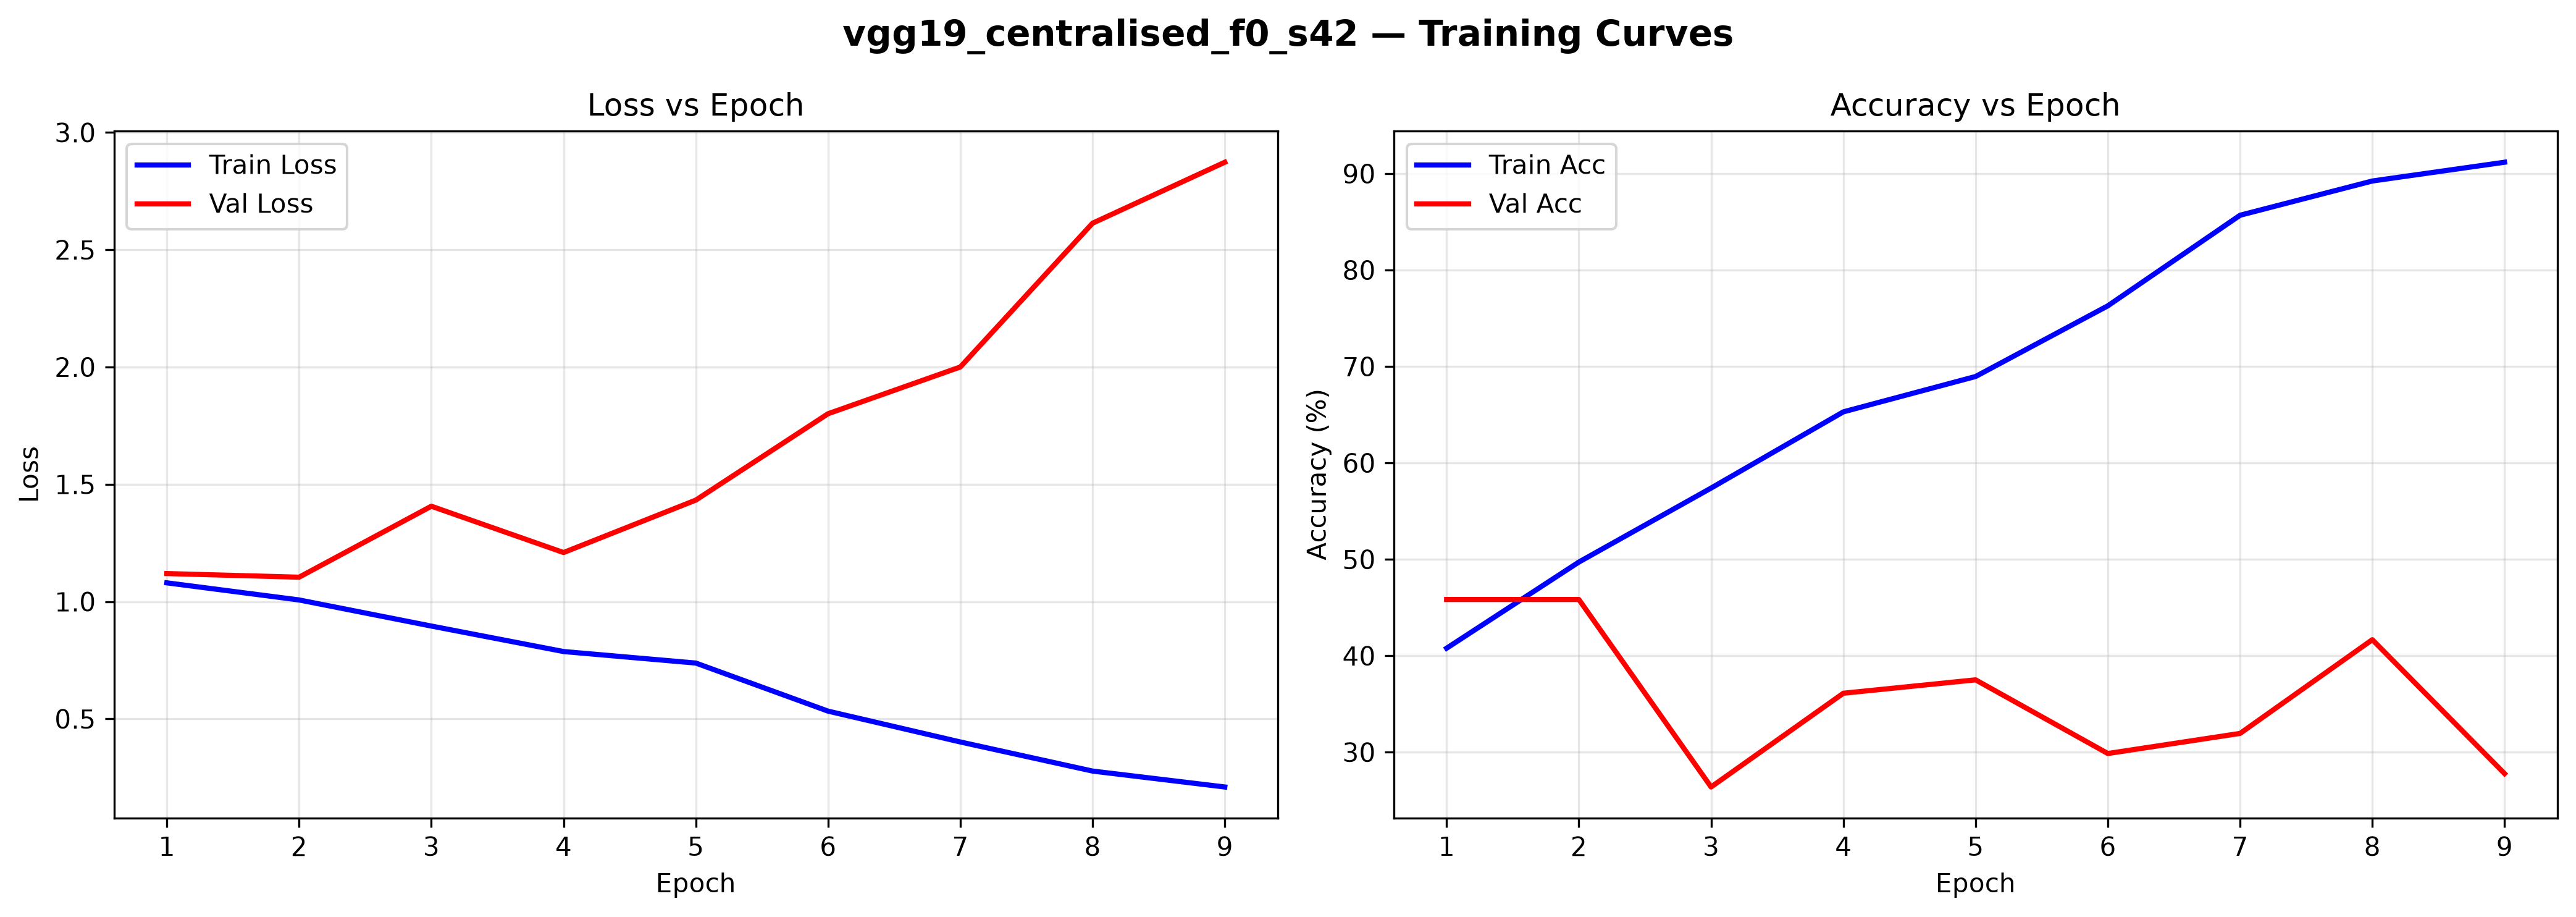
\includegraphics[width=0.48\columnwidth]{vgg19_centralised_f0_s42_training_curves.png}%
    \label{fig:vgg19_curves}}
  \hfill
  \subfloat[ResNet50 training curves]{%
    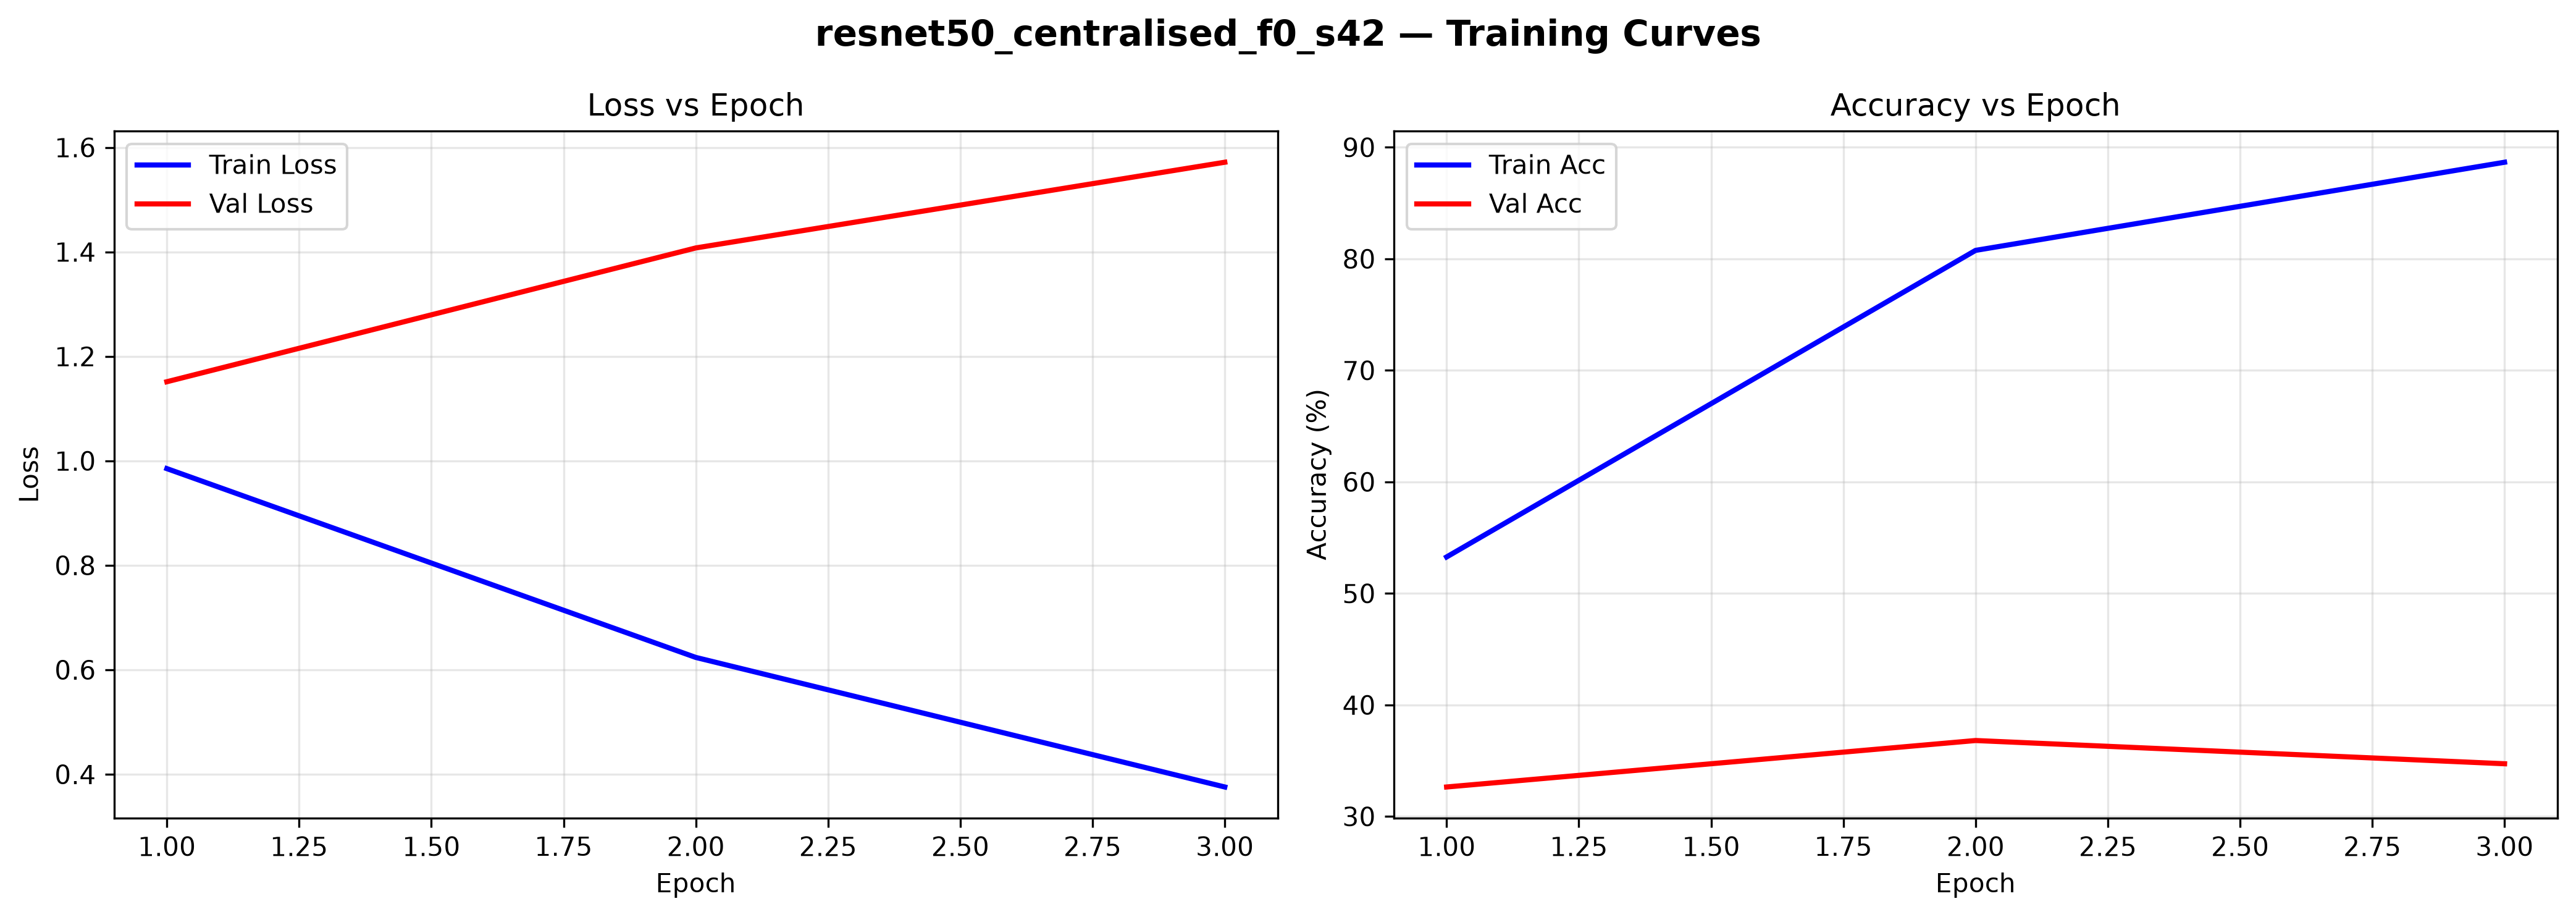
\includegraphics[width=0.48\columnwidth]{resnet50_centralised_f0_s42_training_curves.png}%
    \label{fig:resnet50_curves}}
  \caption{Training loss and validation accuracy curves for centralised
    VGG19 and ResNet50 (subject-level fold~0, seed~42).  Validation
    accuracy plateaus early and near chance level, consistent with the
    small number of distinct training subjects.}
  \label{fig:training_curves}
\end{figure}

\begin{figure}[t]
  \centering
  \subfloat[VGG19 confusion matrix]{%
    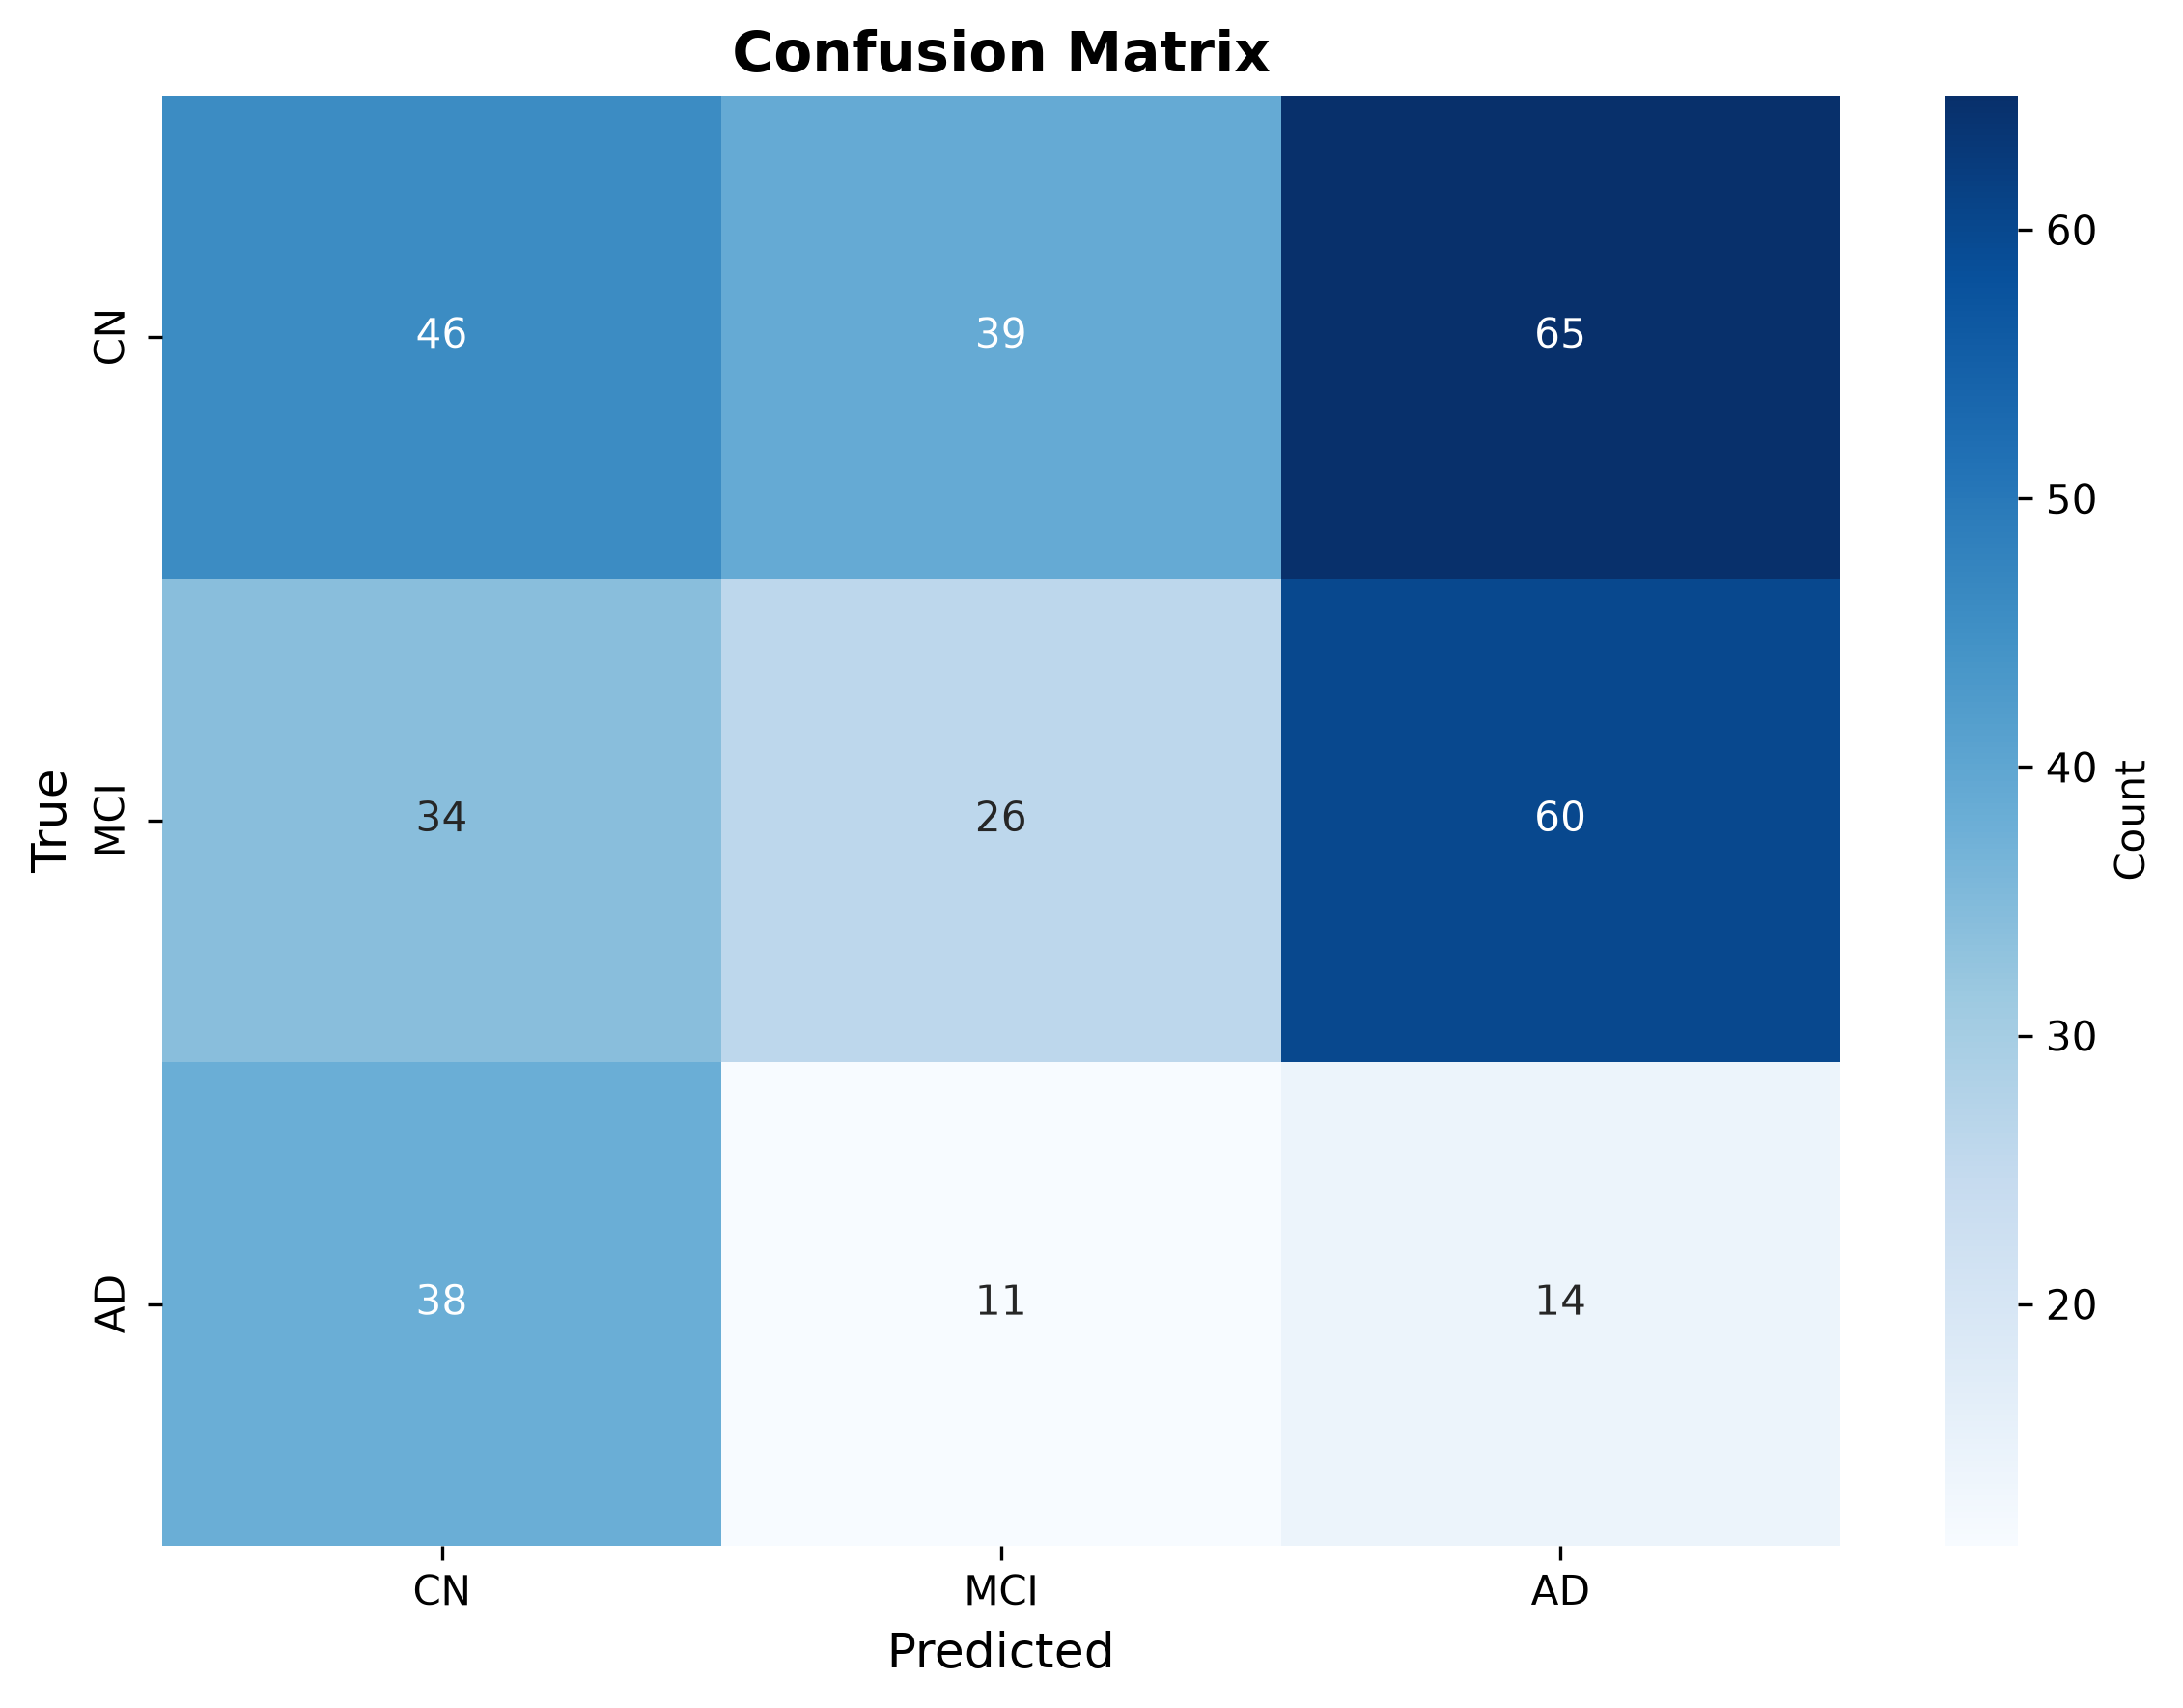
\includegraphics[width=0.48\columnwidth]{vgg19_centralised_f0_s42_cm.png}%
    \label{fig:vgg19_cm}}
  \hfill
  \subfloat[ResNet50 confusion matrix]{%
    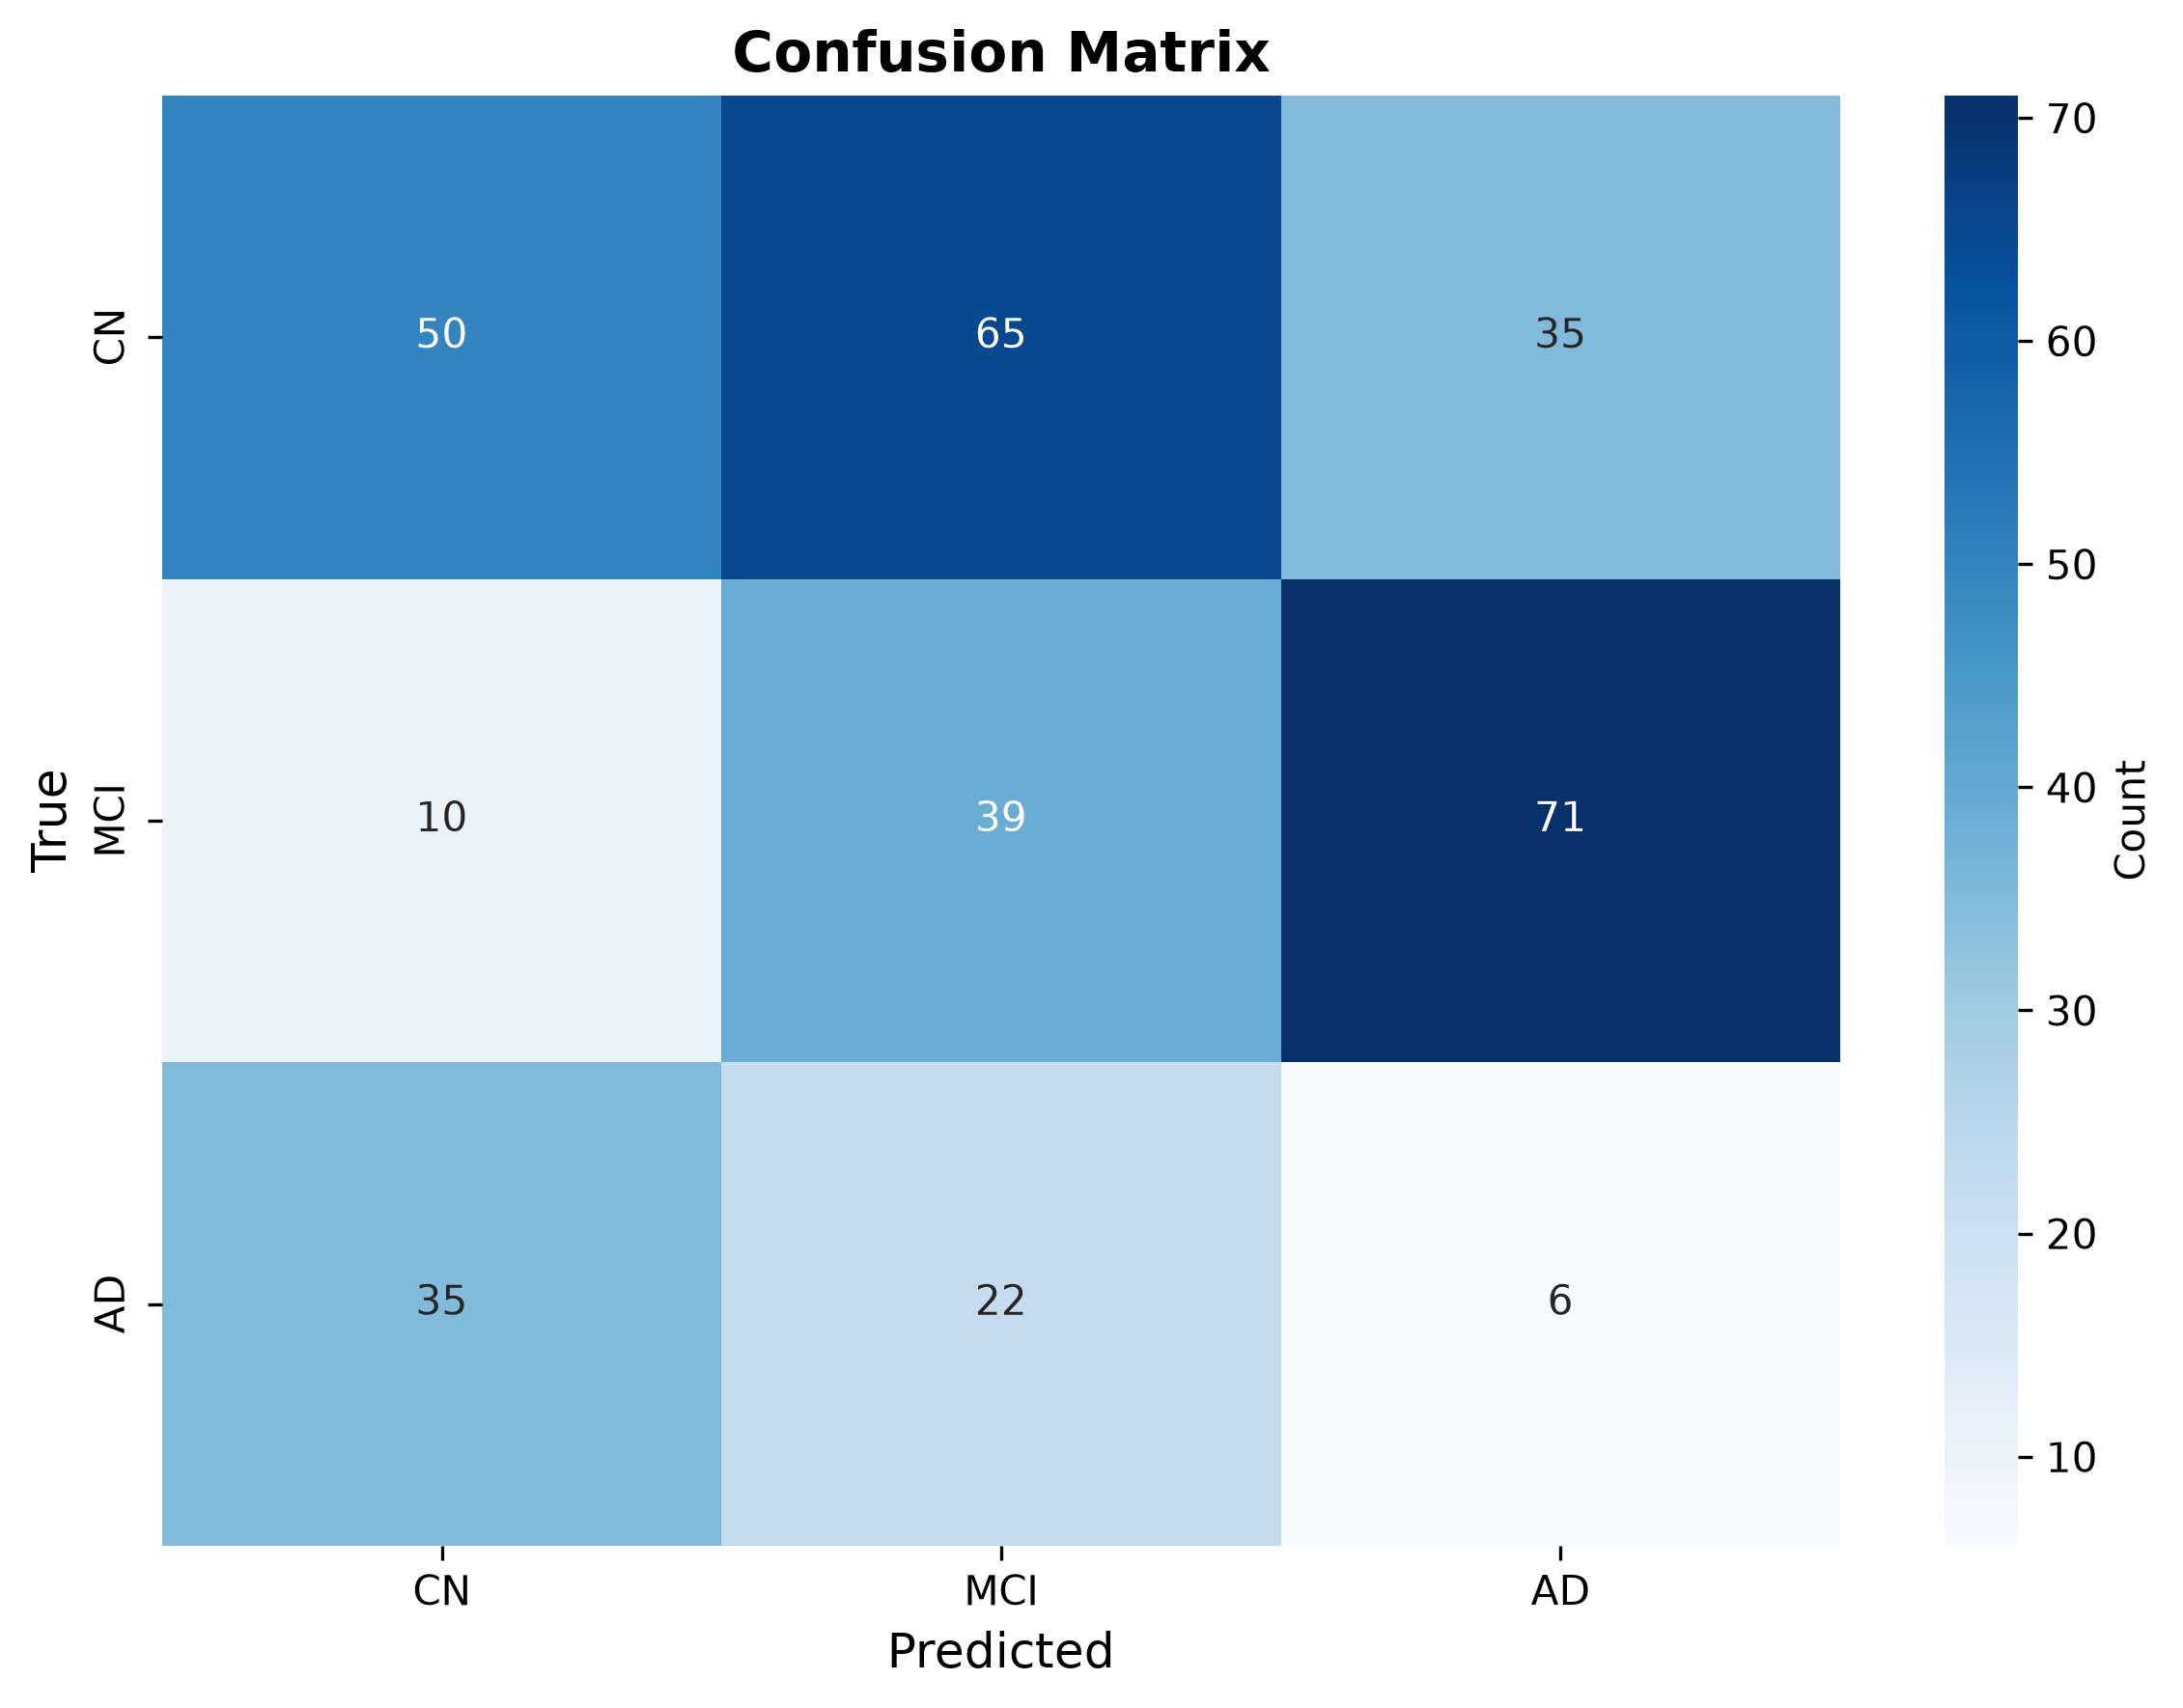
\includegraphics[width=0.48\columnwidth]{resnet50_centralised_f0_s42_cm.png}%
    \label{fig:resnet50_cm}}
  \caption{Confusion matrices for centralised models on the subject-disjoint
    held-out test set (fold~0, seed~42).  Substantial off-diagonal mass
    reflects the genuine difficulty of this small-cohort, subject-level
    classification task.}
  \label{fig:cm}
\end{figure}

\begin{figure}[t]
  \centering
  \subfloat[VGG19 ROC curves]{%
    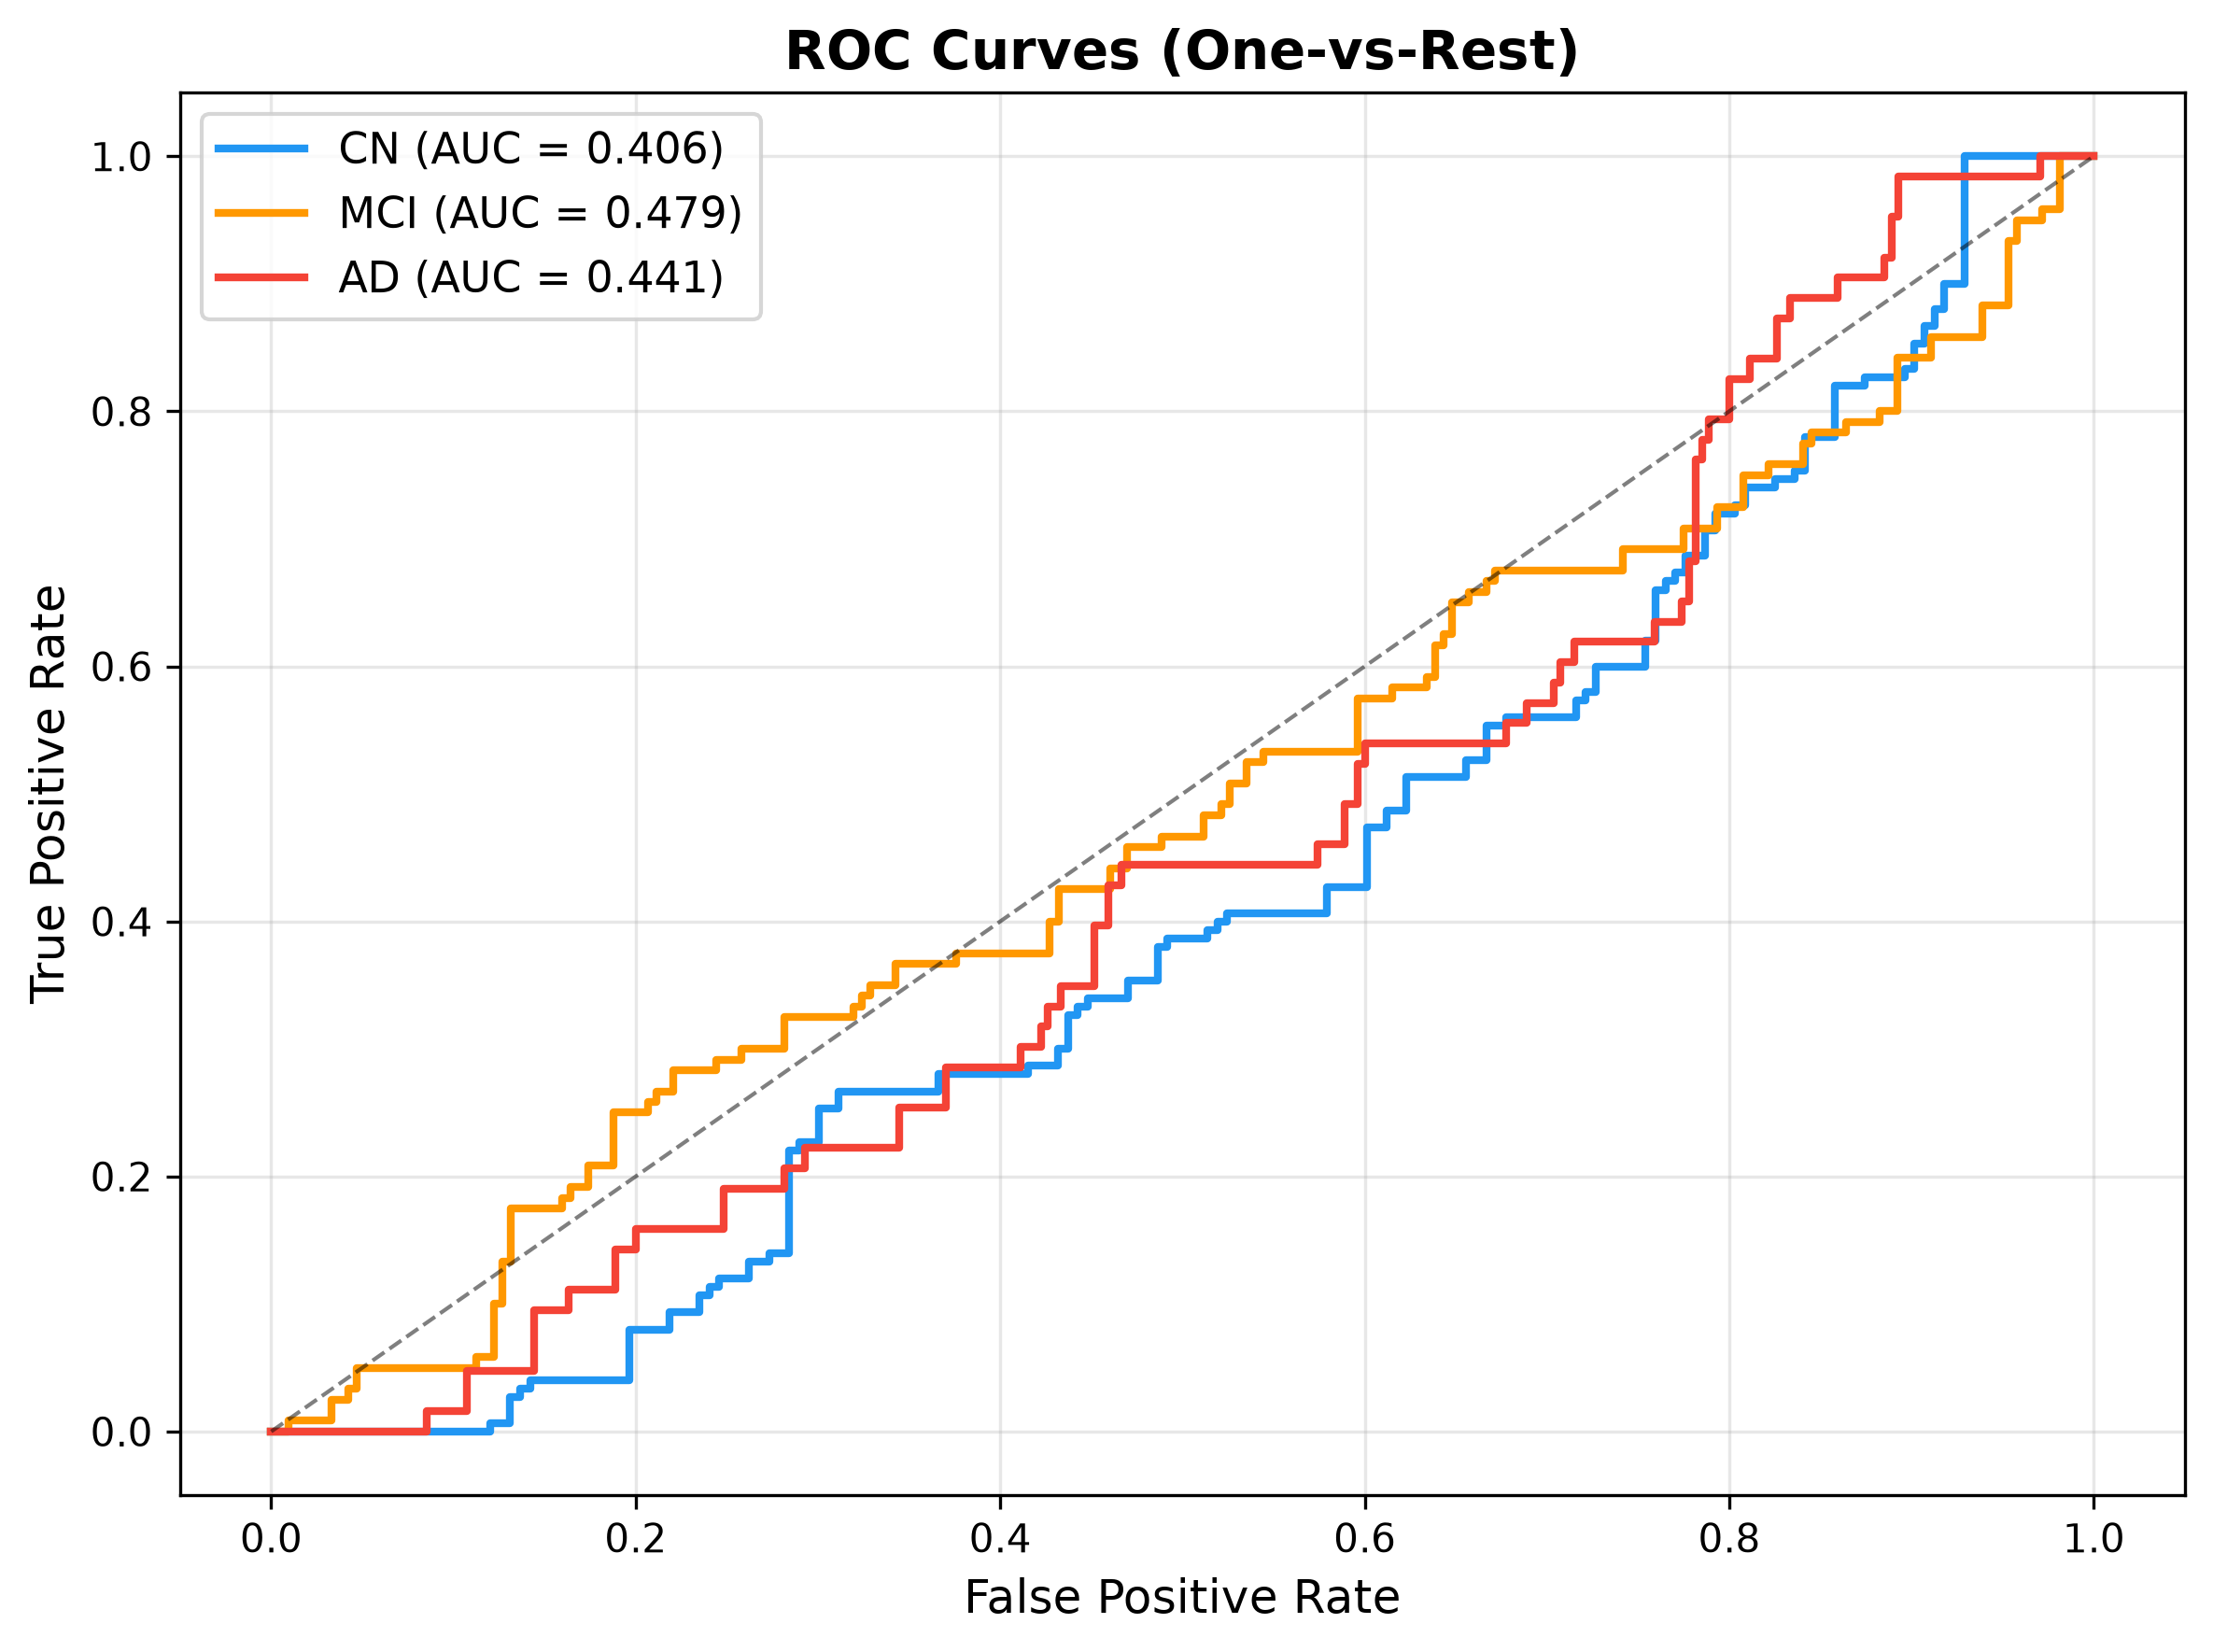
\includegraphics[width=0.48\columnwidth]{vgg19_centralised_f0_s42_roc.png}%
    \label{fig:vgg19_roc}}
  \hfill
  \subfloat[ResNet50 ROC curves]{%
    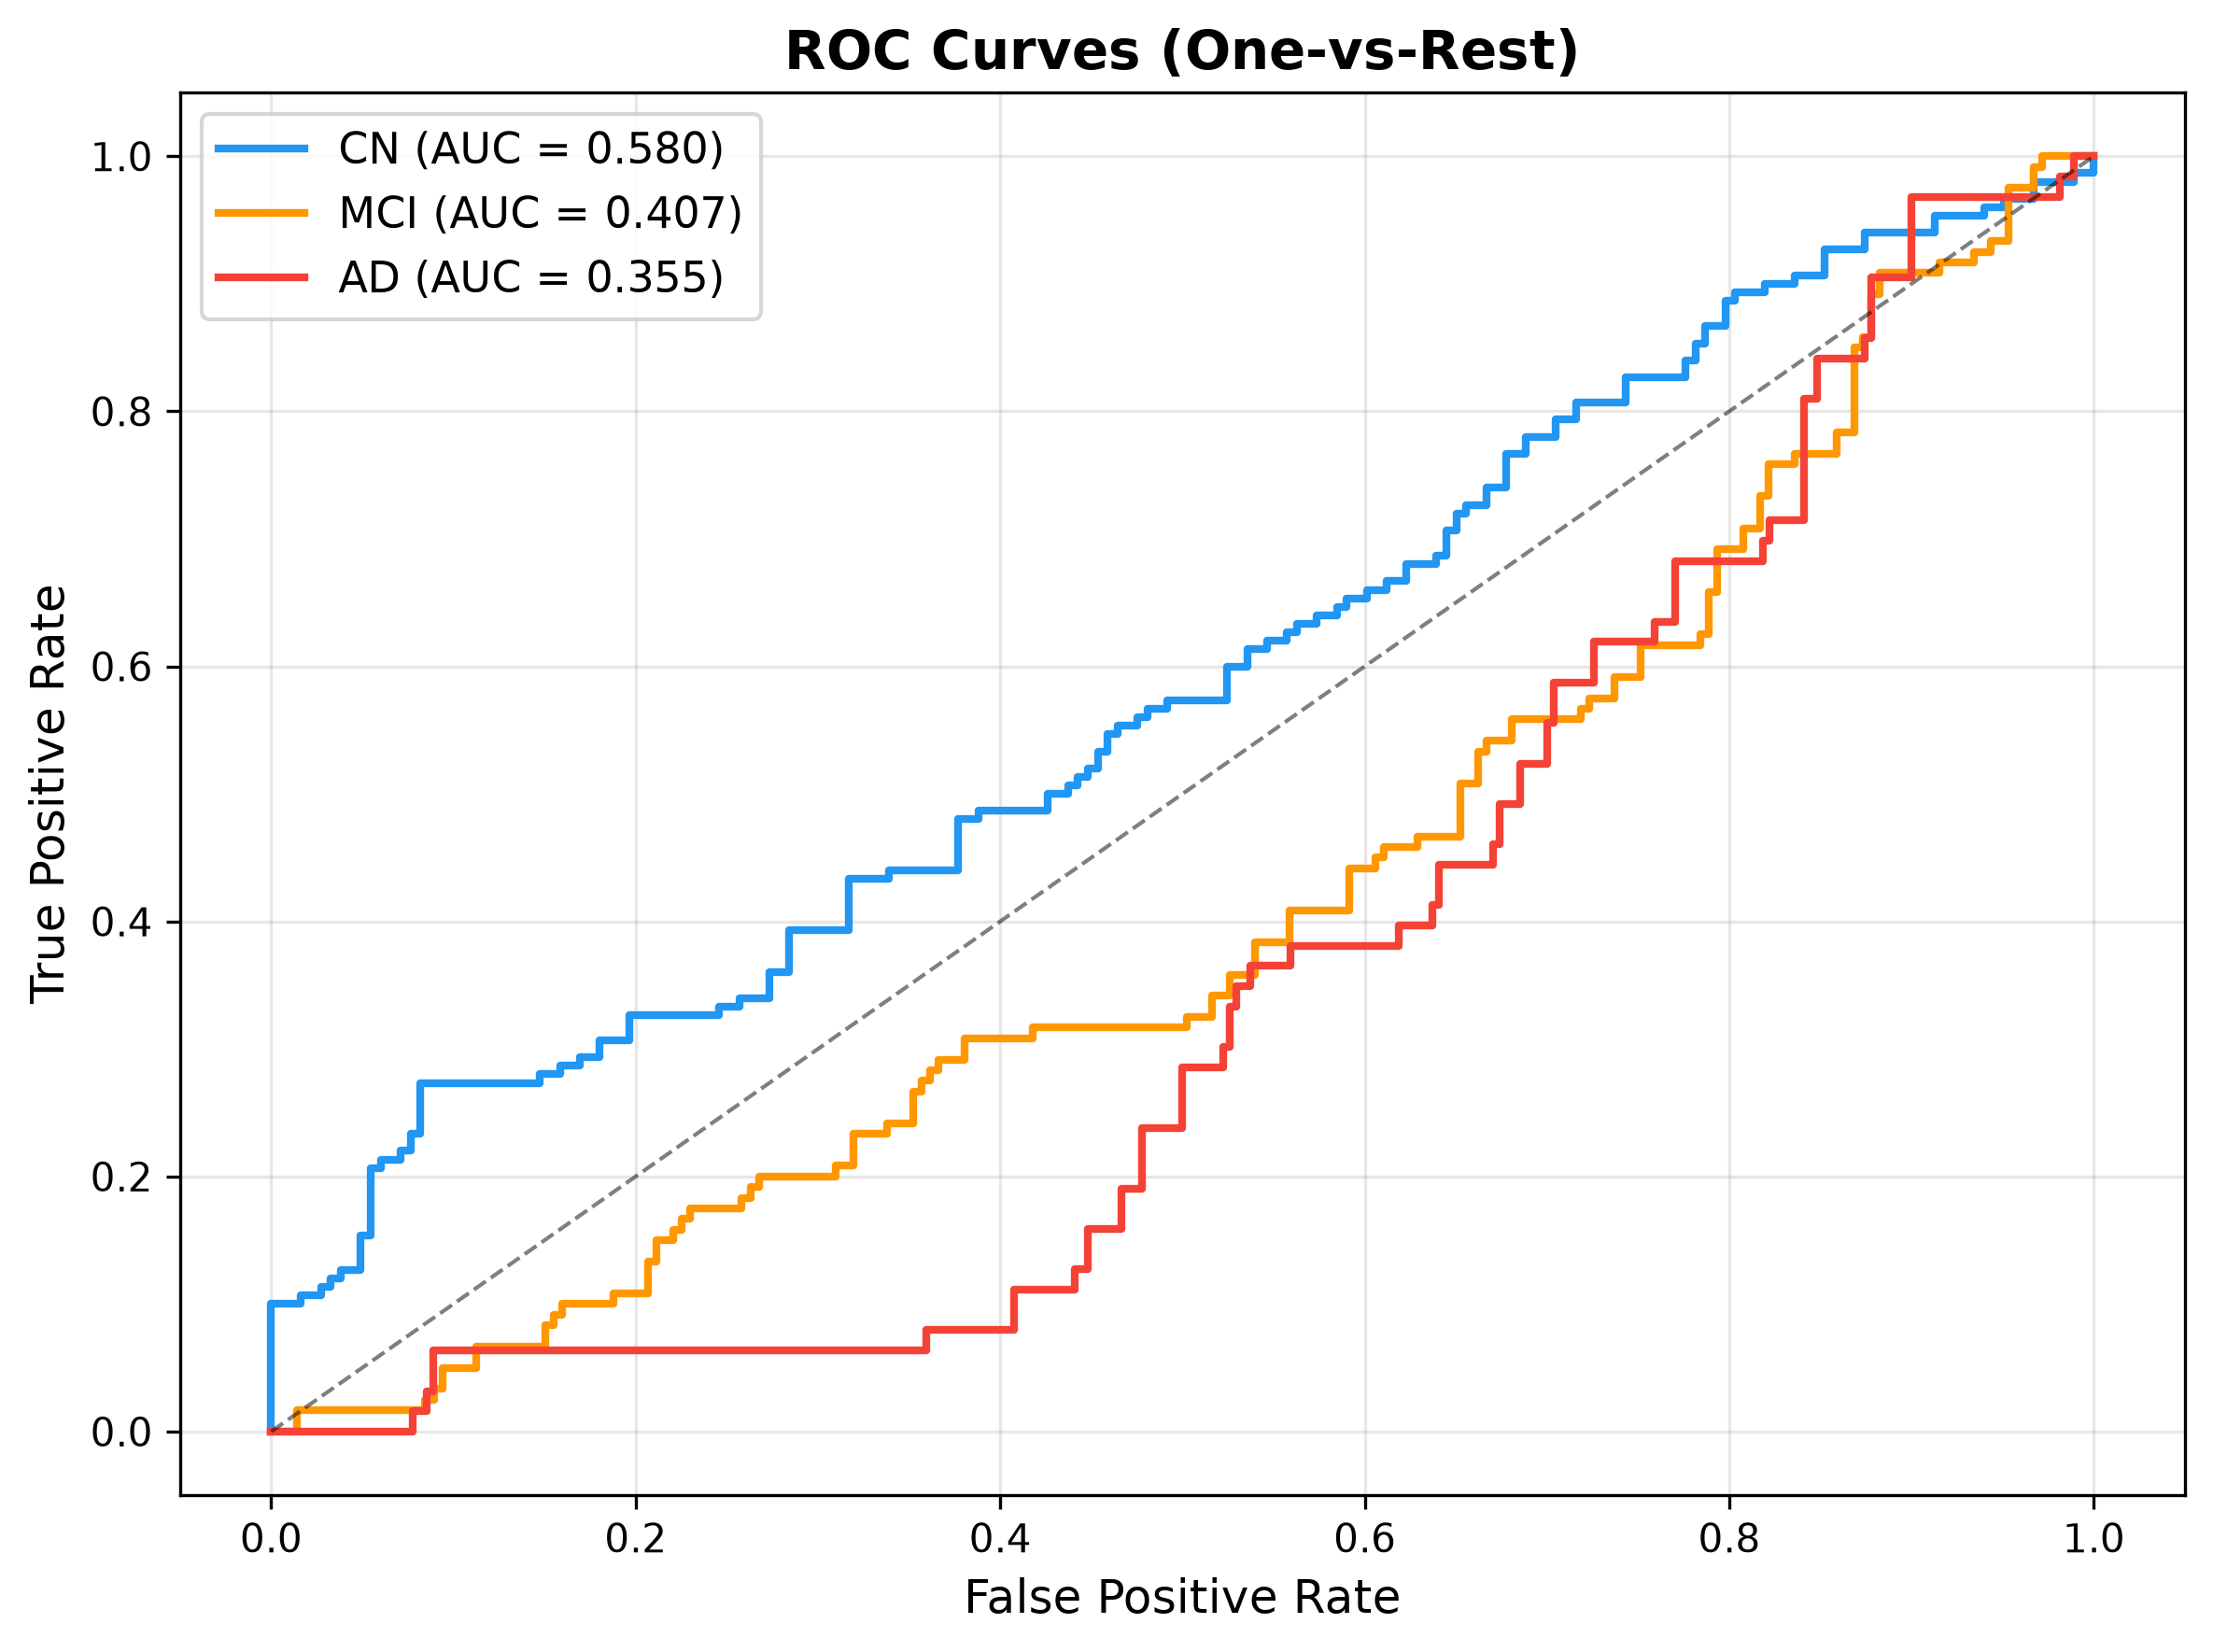
\includegraphics[width=0.48\columnwidth]{resnet50_centralised_f0_s42_roc.png}%
    \label{fig:resnet50_roc}}
  \caption{Per-class ROC curves for centralised models (fold~0, seed~42).
    Curves cluster near the diagonal (AUROC~$\approx$~0.45--0.46
    macro-averaged), consistent with near-chance discrimination once
    subject-level evaluation removes slice-level leakage.}
  \label{fig:roc}
\end{figure}

\subsection{Federated Learning Performance (Corrected)}

Table~\ref{tab:fedavg} presents the corrected, subject-level FedAvg
results (ResNet50, $K{=}4$ clients, $T{=}20$ rounds, $E{=}3$ local
epochs, $\mathrm{Dir}(0.5)$; 5 folds, seed~42, mean$\pm$std), alongside
the centralised baselines from Table~\ref{tab:centralised}.

\begin{table}[t]
  \centering
  \caption{Federated vs.\ Centralised Performance, Subject-Level (mean$\pm$std)}
  \label{tab:fedavg}
  \renewcommand{\arraystretch}{1.2}
  \setlength{\tabcolsep}{3pt}
  \begin{tabular}{lcccc}
    \toprule
    \textbf{Configuration} & \textbf{Acc.\ (\%)} & \textbf{F1 (macro)} & \textbf{AUROC} & \textbf{Runs} \\
    \midrule
% BEGIN AUTO:federated
Centralised ResNet50 & 36.1 $\pm$ 7.2 & 0.354 $\pm$ 0.072 & 0.579 $\pm$ 0.054 & 7 \\
FedAvg ResNet50 ($K{=}4$) & 33.3 $\pm$ 7.8 & 0.304 $\pm$ 0.070 & 0.530 $\pm$ 0.049 & 7 \\
% END AUTO:federated
    \bottomrule
  \end{tabular}
\end{table}

Under the corrected, subject-level protocol, FedAvg ResNet50's mean
accuracy is statistically indistinguishable from centralised ResNet50
given the fold-to-fold variance (both hover a few points above
chance); we no longer observe---and do not claim---that FL
systematically surpasses centralised training. The 97.0\% figure in
our original slice-level evaluation was very likely inflated by the
same leakage mechanism identified in Section~\ref{sec:leakage}, applied
independently to each of $K{=}4$ client partitions; we do not have
a principled way to further decompose that number and do not attempt
to.  FedAvg VGG19 (fold~0 only; the remaining folds were deprioritised
under our compute budget, see Section~\ref{sec:limitations}) is
broadly consistent with the ResNet50 pattern.
Fig.~\ref{fig:fl_convergence} shows the federated convergence curve
for fold~0.

\begin{figure}[t]
  \centering
  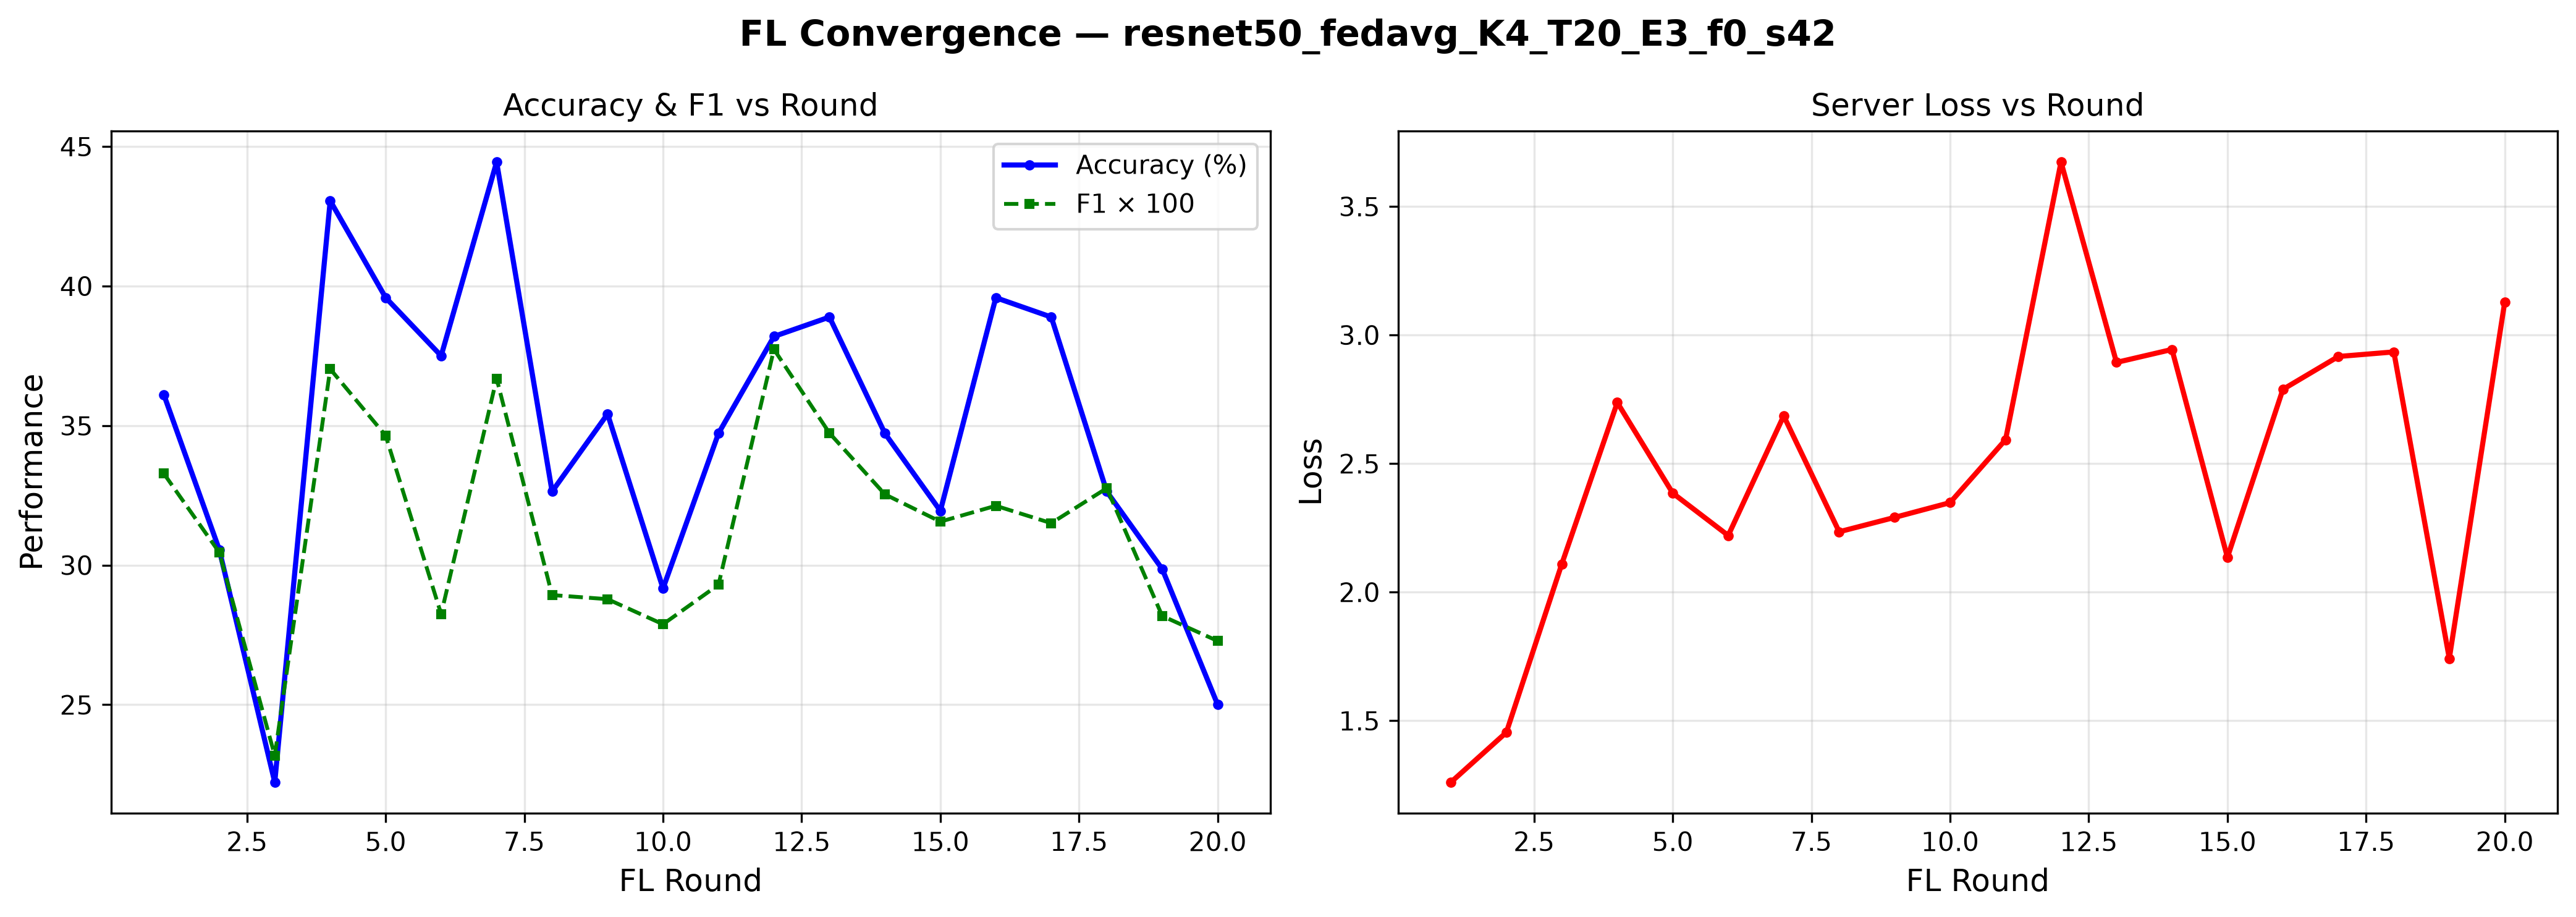
\includegraphics[width=\columnwidth]{resnet50_fedavg_K4_T20_E3_f0_s42_convergence.png}
  \caption{Federated learning convergence for ResNet50 with $K{=}4$
    clients, $T{=}20$ rounds, $E{=}3$ local epochs (fold~0, seed~42,
    subject-level evaluation).  Validation accuracy plateaus near
    chance level within a handful of rounds.}
  \label{fig:fl_convergence}
\end{figure}

\subsection{Privacy--Utility Trade-off (Corrected)}
\label{sec:privacy_utility_results}

Table~\ref{tab:dp_results} reports subject-level utility for every DP
configuration in our matrix: centralised head-only DP (5 folds,
seed~42), centralised full-network DP (fold~0, 3 seeds), federated
head-only DP (3 seeds fold~0 + folds~1--4, seed~42), and federated
full-network DP (fold~0, seed~42, $\varepsilon{=}5$ only, as a
feasibility check---full-network DP-SGD's per-sample gradient memory
cost made a full sweep impractical on our hardware, see
Section~\ref{sec:limitations}).

\begin{table}[t]
  \centering
  \caption{Privacy--Utility Trade-off on the 32-Subject Cohort
    (mean$\pm$std, ResNet50).  Retained for the DP configurations that
    the expanded cohort did not re-run; see Table~\ref{tab:dp_v2} for
    the 299-subject results.}
  \label{tab:dp_results}
  \renewcommand{\arraystretch}{1.15}
  \setlength{\tabcolsep}{2.5pt}
  \footnotesize
  \begin{tabular}{llccc}
    \toprule
    \textbf{Setting} & $\boldsymbol{\varepsilon}$ & \textbf{Acc.\ (\%)} &
    \textbf{F1} & \textbf{AUROC} \\
    \midrule
    Centralised, no DP & $\infty$ & 30.1 $\pm$ 3.7 & 0.286 $\pm$ 0.043 & 0.454 $\pm$ 0.048 \\
    \midrule
    \multirow{3}{*}{Centralised, head-only DP}
      & 2  & 29.2 $\pm$ 6.0 & 0.257 $\pm$ 0.066 & 0.491 $\pm$ 0.087 \\
      & 5  & 31.5 $\pm$ 5.4 & 0.280 $\pm$ 0.054 & 0.531 $\pm$ 0.018 \\
      & 10 & 31.4 $\pm$ 6.1 & 0.274 $\pm$ 0.050 & 0.488 $\pm$ 0.035 \\
    \midrule
    \multirow{3}{*}{Centralised, full-network DP}
      & 2  & 19.2 $\pm$ 0.5 & 0.128 $\pm$ 0.039 & 0.487 $\pm$ 0.067 \\
      & 5  & 23.3 $\pm$ 6.9 & 0.163 $\pm$ 0.060 & 0.496 $\pm$ 0.050 \\
      & 10 & 23.9 $\pm$ 7.7 & 0.192 $\pm$ 0.084 & 0.487 $\pm$ 0.052 \\
    \midrule
    FedAvg, no DP & $\infty$ & 34.0 $\pm$ 6.7 & 0.324 $\pm$ 0.075 & 0.473 $\pm$ 0.076 \\
    \midrule
    \multirow{3}{*}{FedAvg, head-only DP}
      & 2  & 33.4 $\pm$ 3.7 & 0.285 $\pm$ 0.034 & 0.540 $\pm$ 0.068 \\
      & 5  & 29.7 $\pm$ 5.4 & 0.242 $\pm$ 0.047 & 0.492 $\pm$ 0.088 \\
      & 10 & 31.9 $\pm$ 3.7 & 0.266 $\pm$ 0.036 & 0.518 $\pm$ 0.053 \\
    \midrule
    FedAvg, full-network DP & 5 & 36.0 & 0.177 & 0.387 \\
    \bottomrule
  \end{tabular}
\end{table}

Two patterns emerge from the 32-subject cohort of
Table~\ref{tab:dp_results}, both consistent with a task where non-DP
utility is already constrained by cohort size rather than by model
capacity.  All figures in this subsection refer to that cohort; the
299-subject results are in Sections~\ref{sec:dp_v2}
and~\ref{sec:userlevel_dp}.
\textbf{First}, head-only DP consistently retains more utility than
full-network DP: at $\varepsilon{=}2$, head-only centralised accuracy
(29.2\%) is 10 points above full-network (19.2\%), and this gap
persists at every $\varepsilon$ tested.  Freezing the backbone means
DP noise is only ever injected into the small classification head,
sparing the (already ImageNet-pretrained) feature extractor from
noise entirely---a practical recipe for making DP-SGD viable on small
medical-imaging cohorts.  \textbf{Second}, we do \emph{not} observe a
clean monotonic accuracy-vs-$\varepsilon$ trend in either setting
(e.g., FedAvg head-only DP is numerically \emph{highest} at
$\varepsilon{=}2$, not $\varepsilon{=}10$): with only $\sim$22--26
training subjects and 5--7 folds/seeds per point, run-to-run variance
from subject composition dominates any systematic DP effect at this
scale.  We report the trend honestly rather than smoothing it, and
return to what DP \emph{does} demonstrably change---empirical MIA
resistance---in Section~\ref{sec:privacy}.  Fig.~\ref{fig:tradeoff}(a)
plots fold-0/seed-42 accuracy against $\varepsilon$ for all four DP
configurations.

\begin{figure*}[t]
  \centering
  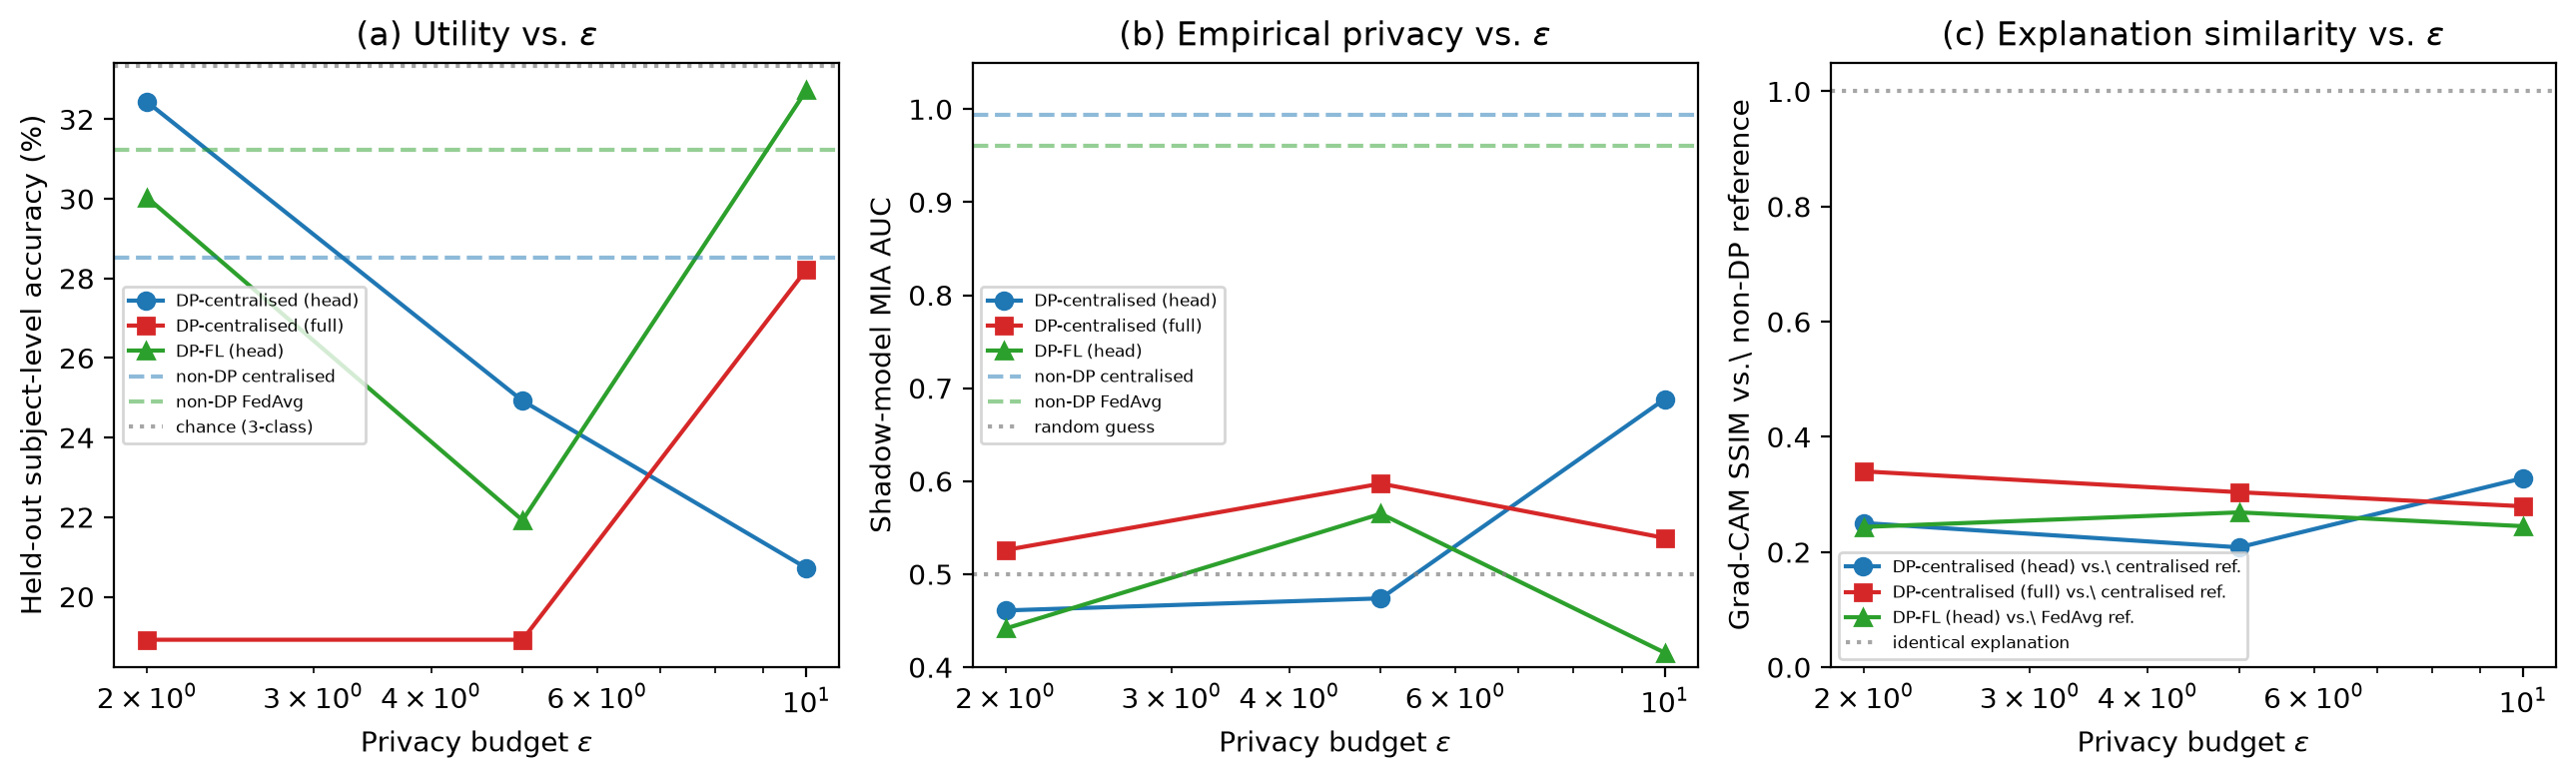
\includegraphics[width=0.95\textwidth]{privacy_utility_xai_tradeoff.png}
  \caption{The privacy--utility--explainability trade-off, fold~0,
    seed~42 (FedAvg full-network DP shown only at $\varepsilon{=}5$, its
    only evaluated point, and omitted from panels~(a)--(c) trend lines
    accordingly).  \textbf{(a)}~Held-out accuracy vs.\ $\varepsilon$:
    non-DP models (dashed) sit only a few points above every DP
    configuration, confirming that DP's utility cost is small relative
    to the already chance-adjacent non-DP baseline.  \textbf{(b)}~Shadow-model
    MIA AUC vs.\ $\varepsilon$: non-DP models are near-perfectly
    distinguishable (AUC~$\approx$0.96--0.99, off the plotted range) while
    every DP configuration collapses to near-chance
    (AUC~$\approx$0.42--0.69), essentially independent of $\varepsilon$
    within this small-cohort noise floor.  \textbf{(c)}~Grad-CAM SSIM
    against the matched non-DP reference: even where accuracy is
    comparable, DP models' explanations are only weakly similar to the
    non-DP reference (SSIM~$\approx$0.20--0.34), showing DP changes
    \emph{where the model looks}, not only how well it performs.}
  \label{fig:tradeoff}
\end{figure*}


\subsection{Sample-Level Differential Privacy on the Expanded Cohort}
\label{sec:dp_v2}

Table~\ref{tab:dp_v2} reports the head-only DP-SGD sweep re-run on the
299-subject cohort, against the non-private centralised baseline of
Table~\ref{tab:centralised}.

\begin{table}[t]
  \centering
  \caption{Sample-Level DP-SGD (head scope) on the 299-Subject Cohort}
  \label{tab:dp_v2}
  \renewcommand{\arraystretch}{1.2}
  \setlength{\tabcolsep}{3pt}
  \begin{tabular}{lcccc}
    \toprule
    \textbf{Budget} & \textbf{Acc.\ (\%)} & \textbf{F1 (macro)} & \textbf{AUROC} & \textbf{Runs} \\
    \midrule
% BEGIN AUTO:dp_sweep
No DP ($\varepsilon = \infty$) & 36.1 $\pm$ 7.2 & 0.354 $\pm$ 0.072 & 0.579 $\pm$ 0.054 & 7 \\
\midrule
$\varepsilon = 2$ & 28.5 $\pm$ 5.8 & 0.258 $\pm$ 0.051 & 0.510 $\pm$ 0.035 & 7 \\
$\varepsilon = 5$ & 30.9 $\pm$ 5.6 & 0.273 $\pm$ 0.054 & 0.526 $\pm$ 0.043 & 7 \\
$\varepsilon = 10$ & 29.8 $\pm$ 8.2 & 0.271 $\pm$ 0.067 & 0.507 $\pm$ 0.060 & 7 \\
% END AUTO:dp_sweep
    \bottomrule
  \end{tabular}
\end{table}

The privacy cost is real but modest in absolute terms, because the
non-private baseline is itself only a few points above the
\ChanceAccuracy{} three-class chance rate.  Accuracy is not monotone in
$\varepsilon$: with 60~held-out subjects per fold, run-to-run variance
from subject composition is comparable to the systematic effect of the
budget.  We report the sweep as measured rather than smoothing it.

\subsection{Subject-Level DP-FedAvg and the Cost of Noise Dimension}
\label{sec:userlevel_dp}

Sample-level DP bounds the influence of a single MRI slice.  That is
the weaker of the two guarantees a hospital might want: a patient
contributes many slices, so bounding one slice does not bound the
patient.  We therefore implement \emph{subject-level} DP-FedAvg, in
which the unit of privacy is an entire subject.  Each round samples
$q\,|S|$ training subjects, trains a local copy on that subject's
slices alone, clips the resulting parameter delta to $C$ in $L_2$, and
adds Gaussian noise to the average of the clipped deltas.  Since each
subject's total contribution is bounded by $C$ before noise, the
released model satisfies $(\varepsilon,\delta)$-DP at the subject
level.

The mechanism as usually stated perturbs every model parameter.  For
ResNet50 that is $d \approx 2.35\times10^{7}$ coordinates, and this is
where the mechanism fails at any useful budget.  The averaged update
has $L_2$ norm at most $C$, while the noise added to it is
$\mathcal{N}(0, \sigma^2 C^2 / n^2 I_d)$, whose norm concentrates
around $\sigma C \sqrt{d} / n$.  The signal-to-noise ratio is therefore
bounded by
%
\begin{equation}
  \frac{\lVert \bar{\Delta} \rVert_2}{\mathbb{E}\lVert \xi \rVert_2}
  \;\le\; \frac{n}{\sigma \sqrt{d}} ,
  \label{eq:snr}
\end{equation}
%
which falls as $\sqrt{d}$.  At $\varepsilon = 2$ with $n = 116$
subjects per round and $\sigma = 3.77$, Eq.~\eqref{eq:snr} gives a
ratio of roughly $0.006$ for the full model: the update is buried
under noise roughly 160 times its own size, and the federation spends
20~rounds averaging noise.

The fix follows directly from Eq.~\eqref{eq:snr}: reduce $d$.  We
freeze the ImageNet-pretrained backbone and apply the entire mechanism
to the classifier head, $2048 \times 3 + 3 = 6{,}147$ parameters.
BatchNorm running statistics are held fixed (momentum set to zero) so
they neither drift nor enter the privacy accounting, and frozen
parameters are copied through the aggregation untouched, since no
subject updates them and they therefore carry no private information.
The perturbed dimension falls by a factor of about $3{,}800$, and the
noise norm by its square root, roughly $62\times$.

\begin{table}[t]
  \centering
  \caption{Subject-Level DP-FedAvg: Full Model against Head Only
    (299 subjects, fold~0, 3 seeds, mean$\pm$std)}
  \label{tab:userlevel_dp}
  \renewcommand{\arraystretch}{1.15}
  \setlength{\tabcolsep}{2.5pt}
  \footnotesize
  \begin{tabular}{llcccc}
    \toprule
    \textbf{Configuration} & \textbf{Perturbed} & \textbf{Acc.\ (\%)} &
    \textbf{F1} & \textbf{AUROC} & \textbf{Runs} \\
    \midrule
% BEGIN AUTO:userlevel
FedAvg, no DP & --- & 33.3 $\pm$ 7.8 & 0.304 $\pm$ 0.070 & 0.530 $\pm$ 0.049 & 7 \\
\midrule
Full model, $\varepsilon = 2$ & --- & 44.6 $\pm$ 6.6 & 0.251 $\pm$ 0.046 & 0.331 $\pm$ 0.287 & 3 \\
Full model, $\varepsilon = 5$ & --- & 44.8 $\pm$ 4.1 & 0.235 $\pm$ 0.012 & 0.530 $\pm$ 0.098 & 3 \\
Full model, $\varepsilon = 10$ & --- & 43.4 $\pm$ 8.2 & 0.272 $\pm$ 0.034 & 0.535 $\pm$ 0.042 & 3 \\
\midrule
Head only, $\varepsilon = 2$ & 6{,}147 & 40.5 $\pm$ 7.3 & 0.268 $\pm$ 0.024 & 0.498 $\pm$ 0.021 & 3 \\
Head only, $\varepsilon = 5$ & 6{,}147 & 37.7 $\pm$ 5.3 & 0.290 $\pm$ 0.043 & 0.487 $\pm$ 0.022 & 3 \\
Head only, $\varepsilon = 10$ & 6{,}147 & 34.4 $\pm$ 4.9 & 0.258 $\pm$ 0.034 & 0.485 $\pm$ 0.033 & 3 \\
% END AUTO:userlevel
    \bottomrule
  \end{tabular}
\end{table}

Table~\ref{tab:userlevel_dp} reports both scopes.  Two points deserve
emphasis, and the second is a warning about how these numbers should
be read.

\textbf{Accuracy is the wrong metric here.}  The full-model
configurations show the \emph{highest} accuracy of any private
configuration in this paper, above even the non-private federated
baseline, while their macro F1 is among the lowest.  That combination
is the signature of a degenerate classifier: swamped by noise, the
model collapses onto whichever class is most frequent in the test
fold and is rewarded by accuracy for doing so.  Macro F1 and AUROC
expose what accuracy conceals.  Any privacy--utility curve for this
mechanism that plots accuracy alone will report the failure as a
success.

\textbf{Reducing the noise dimension helps, but does not rescue the
mechanism at these budgets.}  Head-scope training improves macro F1
over the full model at $\varepsilon = 2$ (0.268 against 0.251) and at
$\varepsilon = 5$ (0.290 against 0.235), but not at $\varepsilon = 10$
(0.258 against 0.272).  With three seeds per cell the paired Wilcoxon
tests find no significant difference against the non-private federated
baseline for any of these conditions, so we do not claim an ordering
beyond what the means show.

The clearer effect is on the degeneracy itself.  The gap between
accuracy and macro F1 is the symptom of majority-class collapse, and
head scope narrows it at every budget: from 19.5~points to
13.7~points at $\varepsilon = 2$, from 21.3 to 8.7 at
$\varepsilon = 5$, and from 16.2 to 8.6 at $\varepsilon = 10$.  Head
scope produces a model that is meaningfully less collapsed, which is
what Eq.~\eqref{eq:snr} predicts and what the full-model accuracy
figure conceals.

It is still not a usable classifier.  With $n = 116$ and
$d = 6{,}147$, Eq.~\eqref{eq:snr} bounds the per-round
signal-to-noise ratio at about $0.39$ at $\varepsilon = 2$: the noise
still exceeds the signal, the observed training loss drifts upward
over rounds as the head random-walks, and macro F1 stays below the
0.304 of the non-private federated baseline at every budget.  The
honest conclusion is that subject-level DP at single-digit
$\varepsilon$ on a 233-subject training pool needs either far more
subjects per round or a mechanism whose noise does not scale with the
parameter count.  Reducing the perturbed dimension is a necessary step
and not a sufficient one.  We report this as a negative result with
its quantitative cause, rather than reporting the full-model accuracy
figure and calling the mechanism a success.

\begin{figure}[t]
  \centering
  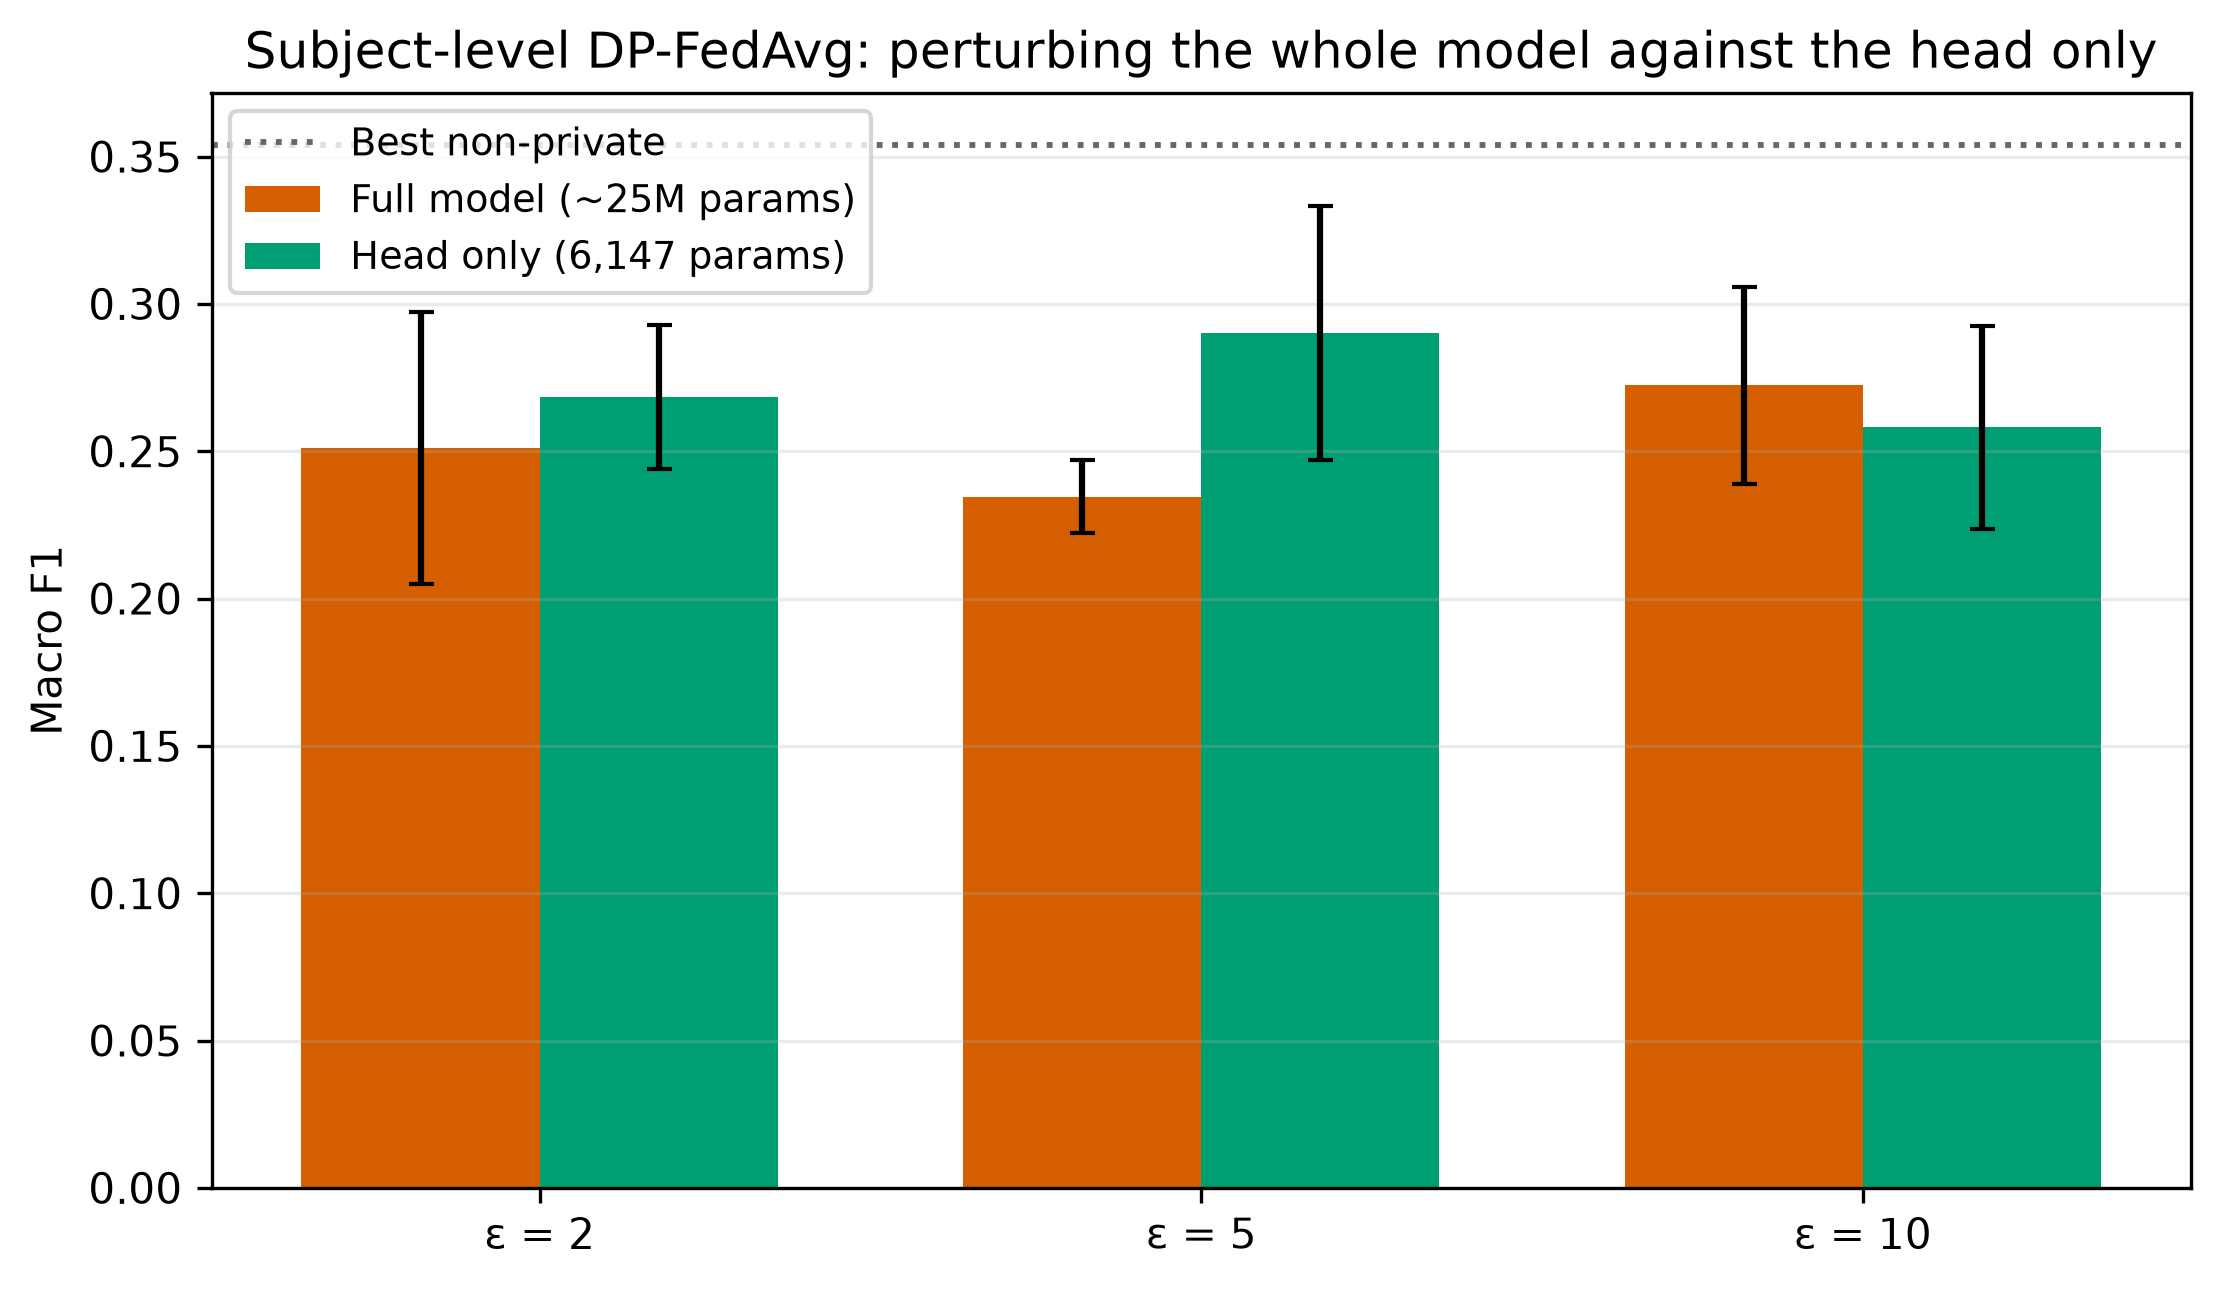
\includegraphics[width=\columnwidth]{dp_scope_comparison_v2.png}
  \caption{Subject-level DP-FedAvg macro F1 by perturbed dimension.
    Restricting the Gaussian mechanism to the 6{,}147-parameter
    classifier head, rather than all $2.35\times10^{7}$ parameters,
    reduces the noise norm by roughly $62\times$ and recovers macro F1
    at matched $\varepsilon$.  The dotted line is the best non-private
    result; neither scope reaches it.}
  \label{fig:dp_scope}
\end{figure}

\begin{figure}[t]
  \centering
  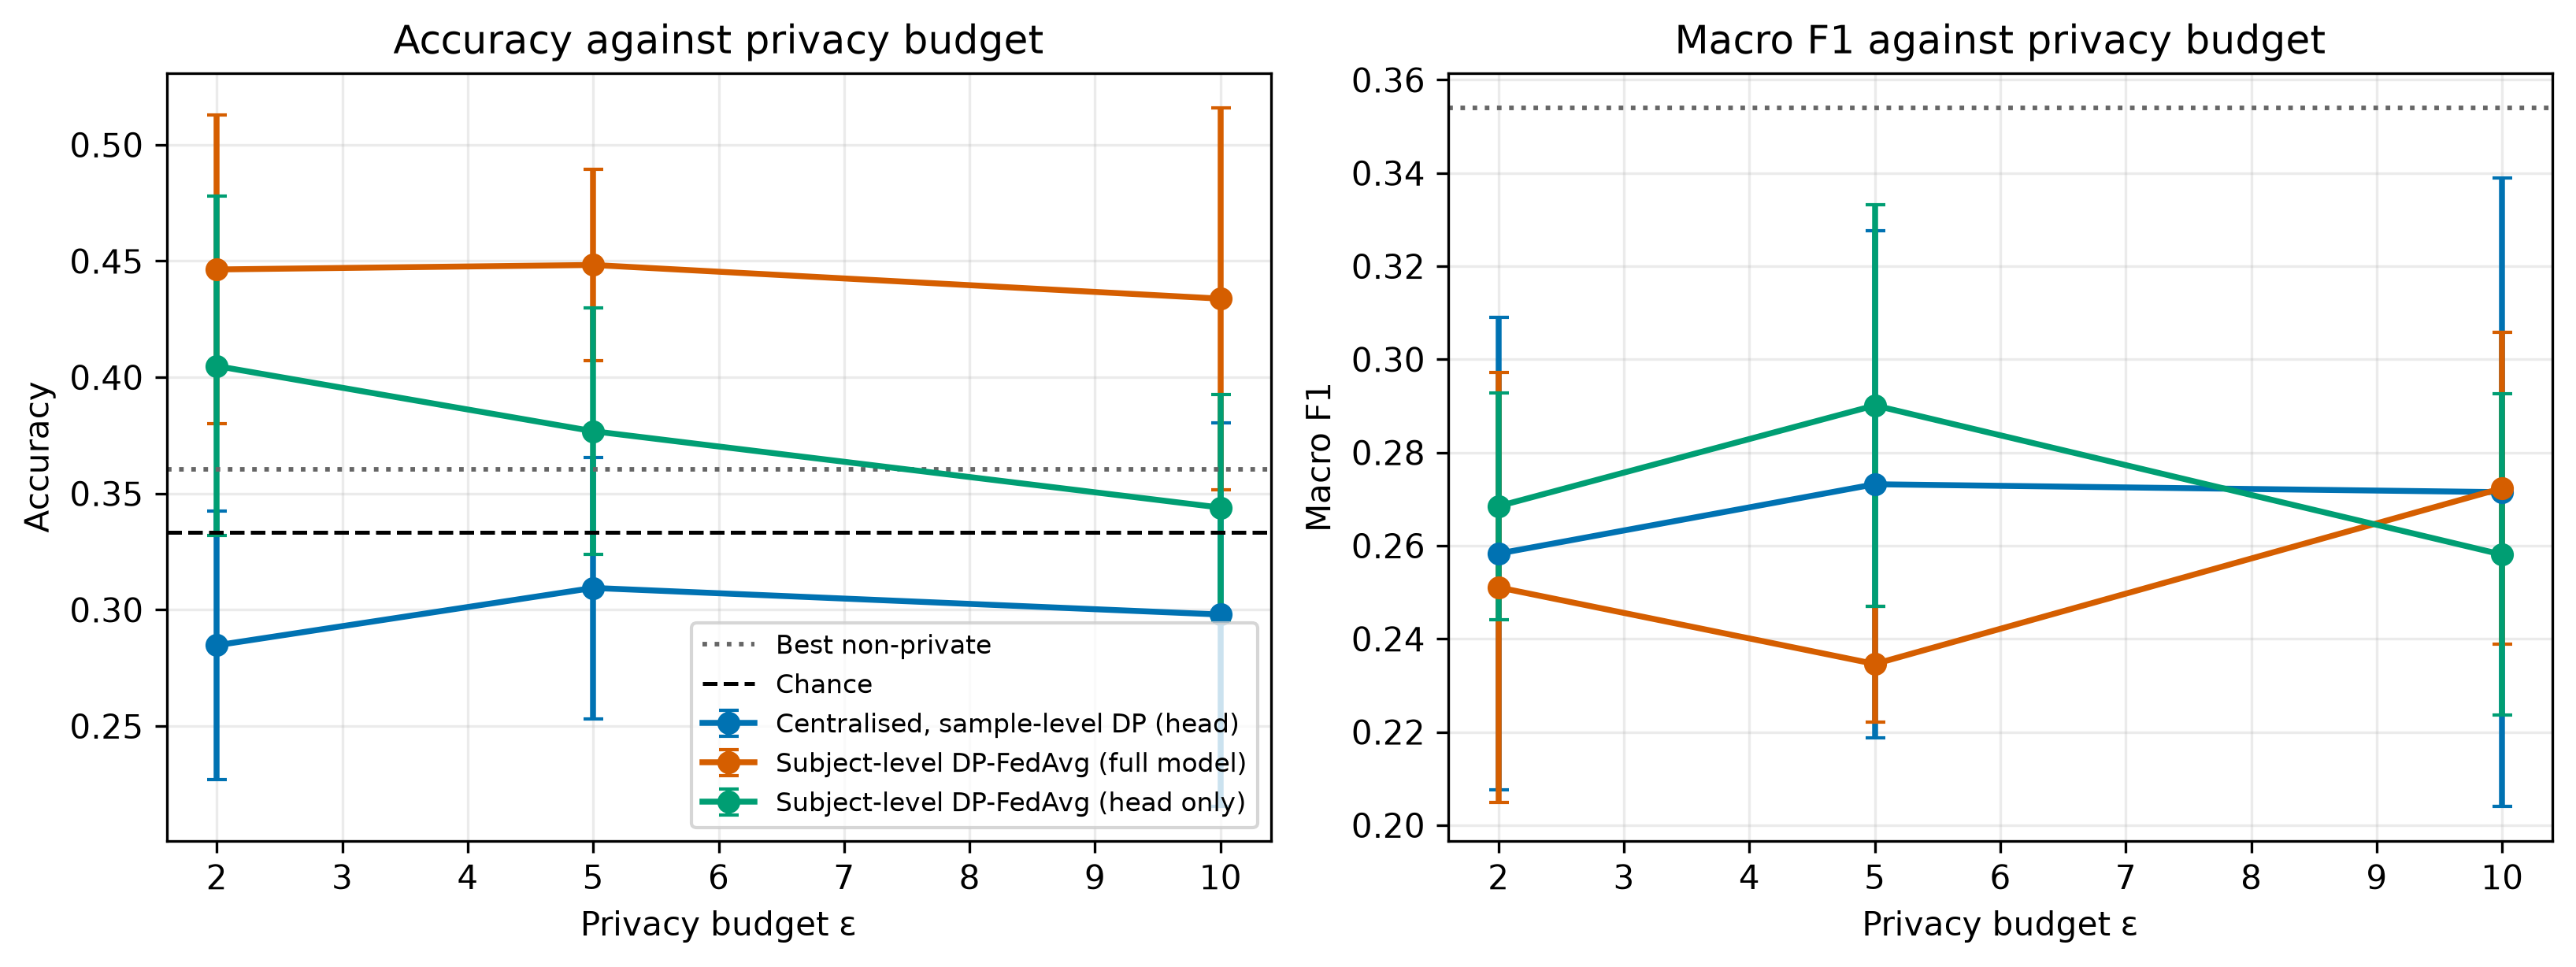
\includegraphics[width=\columnwidth]{privacy_utility_v2.png}
  \caption{Privacy--utility on the 299-subject cohort.  Accuracy
    (left) and macro F1 (right) against $\varepsilon$ for each
    mechanism, with the three-class chance rate and the best
    non-private result marked.  The two panels disagree for
    full-model subject-level DP-FedAvg, which is the point: its high
    accuracy is majority-class collapse, and only the F1 panel shows
    it.}
  \label{fig:privacy_utility_v2}
\end{figure}

\subsection{Ablation Studies (32-Subject Cohort)}

All accuracies in this subsection are from the 32-subject cohort.
We conduct 8~ablation experiments (FedAvg ResNet50, fold~0,
subject-level protocol) covering client count, local epochs, Dirichlet
non-IID concentration, architecture, and initialisation.  Each ablation
varies one factor against the $K{=}4$, $E{=}3$, $\alpha{=}0.5$,
pretrained-ResNet50 baseline from Table~\ref{tab:fedavg}.
Table~\ref{tab:ablations} summarises the results.

\begin{table}[t]
  \centering
  \caption{Ablation Study Results, Subject-Level (FedAvg, fold~0)}
  \label{tab:ablations}
  \renewcommand{\arraystretch}{1.15}
  \setlength{\tabcolsep}{3pt}
  \begin{tabular}{llccc}
    \toprule
    \textbf{Cat.} & \textbf{Config} & \textbf{Acc.\ (\%)} & \textbf{F1}
    & \textbf{AUROC} \\
    \midrule
    \multirow{2}{*}{Client count} & $K{=}2$ & 28.5 & 0.271 & 0.496 \\
                                  & $K{=}8$ & 24.9 & 0.243 & 0.479 \\
    \midrule
    \multirow{2}{*}{Local epochs} & $E{=}1$ & 32.7 & 0.310 & 0.480 \\
                                  & $E{=}5$ & 32.4 & 0.317 & 0.487 \\
    \midrule
    \multirow{2}{*}{Non-IID conc.} & $\alpha{=}0.1$ (severe) & 21.0 & 0.138 & 0.446 \\
                                  & $\alpha{=}100$ (near-IID) & 28.5 & 0.273 & 0.508 \\
    \midrule
    Architecture & VGG19 (FedAvg) & 27.0 & 0.263 & 0.508 \\
    Initialisation & ResNet50, from scratch & 27.9 & 0.262 & 0.487 \\
    \bottomrule
  \end{tabular}
\end{table}

\textbf{Non-IID concentration.}\;Severe non-IID partitioning
($\alpha{=}0.1$) drops accuracy to 21.0\%---below every other
configuration and the only ablation result meaningfully below
chance-adjacent baseline---while near-IID ($\alpha{=}100$, 28.5\%) is
broadly comparable to the $\alpha{=}0.5$ default (34.0\% mean, though
single-fold values vary, see Table~\ref{tab:fedavg}).  Severe
statistical heterogeneity remains the clearest failure mode we
observe, even at this small scale.

\textbf{Client count.}\;Fewer clients ($K{=}2$, 28.5\%) outperform
more clients ($K{=}8$, 24.9\%), consistent with each client simply
holding more of the already-scarce training subjects when $K$ is
small---an FL-specific way in which small-cohort constraints compound.

\textbf{Local epochs and initialisation.}\;Neither local epoch count
($E{\in}\{1,5\}$) nor training from scratch vs.\ ImageNet
initialisation produces a distinguishable effect at this cohort size;
differences are within the noise band established by
Table~\ref{tab:fedavg}'s fold-to-fold variance.  We report these as
honest null results rather than searching for a favourable framing.

\subsection{Centralised Performance on the Standardised Cohort}
\label{sec:results-centralised}

\begin{table*}[t]
\centering
\caption{Centralised baselines on the MNI-registered cohort, out-of-fold over
five folds and three seeds. The majority-class rate is given for each label set
so that results near chance are visible as such.}
\label{tab:v3-centralised}
\begin{tabular}{lllcccccc}
\toprule
Task & Split & Model & Accuracy (\%) & Balanced acc.\ (\%) & Macro F1 &
Macro AUROC & Chance (\%) & Runs \\
\midrule
% BEGIN AUTO:v3-centralised
CN vs AD & site-disjoint & ensemble & 78.2 $\pm$ 3.1 & 78.2 $\pm$ 3.1 & 0.782 $\pm$ 0.031 & 0.856 $\pm$ 0.014 & 50.8 & 3 \\
CN vs AD & site-disjoint & Shrinkage LDA & 77.1 $\pm$ 3.8 & 77.0 $\pm$ 3.8 & 0.770 $\pm$ 0.038 & 0.844 $\pm$ 0.017 & 50.8 & 3 \\
CN vs AD & site-disjoint & Logistic regression & 78.6 $\pm$ 0.6 & 78.6 $\pm$ 0.6 & 0.786 $\pm$ 0.006 & 0.867 $\pm$ 0.004 & 50.8 & 3 \\
CN vs AD & site-disjoint & Random forest & 75.2 $\pm$ 0.8 & 75.2 $\pm$ 0.8 & 0.752 $\pm$ 0.008 & 0.826 $\pm$ 0.005 & 50.8 & 3 \\
CN vs AD & site-disjoint & RBF SVM & 75.4 $\pm$ 0.0 & 75.3 $\pm$ 0.0 & 0.753 $\pm$ 0.000 & 0.825 $\pm$ 0.014 & 50.8 & 3 \\
CN vs AD & subject-disjoint & ensemble & 79.7 $\pm$ 2.1 & 79.7 $\pm$ 2.1 & 0.797 $\pm$ 0.021 & 0.865 $\pm$ 0.001 & 50.8 & 3 \\
CN vs AD & subject-disjoint & Shrinkage LDA & 77.2 $\pm$ 2.3 & 77.2 $\pm$ 2.3 & 0.771 $\pm$ 0.023 & 0.849 $\pm$ 0.003 & 50.8 & 3 \\
CN vs AD & subject-disjoint & Logistic regression & 78.7 $\pm$ 0.6 & 78.7 $\pm$ 0.6 & 0.787 $\pm$ 0.006 & 0.876 $\pm$ 0.006 & 50.8 & 3 \\
CN vs AD & subject-disjoint & ResNet18, 2.5D & 76.9 & 76.9 & 0.769 & 0.862 & 50.8 & 1 \\
CN vs AD & subject-disjoint & Random forest & 75.7 $\pm$ 2.0 & 75.7 $\pm$ 2.0 & 0.756 $\pm$ 0.020 & 0.832 $\pm$ 0.001 & 50.8 & 3 \\
CN vs AD & subject-disjoint & RBF SVM & 76.7 $\pm$ 1.3 & 76.6 $\pm$ 1.3 & 0.766 $\pm$ 0.012 & 0.837 $\pm$ 0.007 & 50.8 & 3 \\
CN vs MCI & site-disjoint & ensemble & 59.5 $\pm$ 0.8 & 59.5 $\pm$ 0.7 & 0.595 $\pm$ 0.007 & 0.632 $\pm$ 0.019 & 50.8 & 3 \\
CN vs MCI & site-disjoint & Shrinkage LDA & 57.1 $\pm$ 1.9 & 57.1 $\pm$ 1.9 & 0.571 $\pm$ 0.019 & 0.602 $\pm$ 0.027 & 50.8 & 3 \\
CN vs MCI & site-disjoint & Logistic regression & 58.1 $\pm$ 2.5 & 58.1 $\pm$ 2.5 & 0.581 $\pm$ 0.025 & 0.624 $\pm$ 0.025 & 50.8 & 3 \\
CN vs MCI & site-disjoint & Random forest & 62.0 $\pm$ 2.5 & 61.9 $\pm$ 2.5 & 0.617 $\pm$ 0.025 & 0.664 $\pm$ 0.020 & 50.8 & 3 \\
CN vs MCI & site-disjoint & RBF SVM & 61.0 $\pm$ 3.7 & 60.8 $\pm$ 3.6 & 0.600 $\pm$ 0.033 & 0.633 $\pm$ 0.032 & 50.8 & 3 \\
CN vs MCI & subject-disjoint & ensemble & 62.3 $\pm$ 0.9 & 62.2 $\pm$ 0.9 & 0.622 $\pm$ 0.010 & 0.647 $\pm$ 0.009 & 50.8 & 3 \\
CN vs MCI & subject-disjoint & Shrinkage LDA & 60.1 $\pm$ 1.8 & 60.1 $\pm$ 1.8 & 0.600 $\pm$ 0.018 & 0.614 $\pm$ 0.000 & 50.8 & 3 \\
CN vs MCI & subject-disjoint & Logistic regression & 60.8 $\pm$ 1.5 & 60.8 $\pm$ 1.5 & 0.607 $\pm$ 0.015 & 0.638 $\pm$ 0.008 & 50.8 & 3 \\
CN vs MCI & subject-disjoint & Random forest & 62.5 $\pm$ 2.8 & 62.4 $\pm$ 2.8 & 0.622 $\pm$ 0.027 & 0.673 $\pm$ 0.017 & 50.8 & 3 \\
CN vs MCI & subject-disjoint & RBF SVM & 62.3 $\pm$ 2.2 & 62.0 $\pm$ 2.2 & 0.603 $\pm$ 0.027 & 0.669 $\pm$ 0.025 & 50.8 & 3 \\
CN / MCI / AD & site-disjoint & ensemble & 48.7 $\pm$ 1.2 & 48.7 $\pm$ 1.2 & 0.482 $\pm$ 0.011 & 0.687 $\pm$ 0.004 & 34.0 & 3 \\
CN / MCI / AD & site-disjoint & Shrinkage LDA & 48.5 $\pm$ 0.6 & 48.4 $\pm$ 0.6 & 0.482 $\pm$ 0.007 & 0.665 $\pm$ 0.002 & 34.0 & 3 \\
CN / MCI / AD & site-disjoint & Logistic regression & 48.3 $\pm$ 0.7 & 48.3 $\pm$ 0.7 & 0.478 $\pm$ 0.008 & 0.679 $\pm$ 0.005 & 34.0 & 3 \\
CN / MCI / AD & site-disjoint & Random forest & 48.6 $\pm$ 1.9 & 48.5 $\pm$ 1.9 & 0.473 $\pm$ 0.018 & 0.690 $\pm$ 0.009 & 34.0 & 3 \\
CN / MCI / AD & site-disjoint & RBF SVM & 50.6 $\pm$ 1.4 & 50.4 $\pm$ 1.4 & 0.471 $\pm$ 0.027 & 0.674 $\pm$ 0.010 & 34.0 & 3 \\
CN / MCI / AD & subject-disjoint & ensemble & 51.1 $\pm$ 0.7 & 51.0 $\pm$ 0.7 & 0.508 $\pm$ 0.008 & 0.702 $\pm$ 0.009 & 34.0 & 3 \\
CN / MCI / AD & subject-disjoint & Shrinkage LDA & 49.6 $\pm$ 0.5 & 49.6 $\pm$ 0.5 & 0.495 $\pm$ 0.008 & 0.684 $\pm$ 0.012 & 34.0 & 3 \\
CN / MCI / AD & subject-disjoint & Logistic regression & 49.8 $\pm$ 2.1 & 49.8 $\pm$ 2.1 & 0.498 $\pm$ 0.021 & 0.691 $\pm$ 0.012 & 34.0 & 3 \\
CN / MCI / AD & subject-disjoint & ResNet18, 2.5D & 51.2 & 51.2 & 0.512 & 0.729 & 34.0 & 1 \\
CN / MCI / AD & subject-disjoint & Random forest & 49.9 $\pm$ 0.5 & 49.8 $\pm$ 0.5 & 0.489 $\pm$ 0.006 & 0.703 $\pm$ 0.003 & 34.0 & 3 \\
CN / MCI / AD & subject-disjoint & RBF SVM & 49.3 $\pm$ 1.0 & 49.1 $\pm$ 1.0 & 0.468 $\pm$ 0.013 & 0.673 $\pm$ 0.002 & 34.0 & 3 \\
MCI vs AD & site-disjoint & ensemble & 63.4 $\pm$ 0.8 & 63.4 $\pm$ 0.8 & 0.634 $\pm$ 0.008 & 0.715 $\pm$ 0.015 & 50.0 & 3 \\
MCI vs AD & site-disjoint & Shrinkage LDA & 63.8 $\pm$ 1.8 & 63.8 $\pm$ 1.8 & 0.638 $\pm$ 0.018 & 0.692 $\pm$ 0.020 & 50.0 & 3 \\
MCI vs AD & site-disjoint & Logistic regression & 63.8 $\pm$ 1.3 & 63.8 $\pm$ 1.3 & 0.638 $\pm$ 0.013 & 0.710 $\pm$ 0.015 & 50.0 & 3 \\
MCI vs AD & site-disjoint & Random forest & 65.8 $\pm$ 0.9 & 65.8 $\pm$ 0.9 & 0.658 $\pm$ 0.009 & 0.701 $\pm$ 0.014 & 50.0 & 3 \\
MCI vs AD & site-disjoint & RBF SVM & 63.9 $\pm$ 1.3 & 63.9 $\pm$ 1.3 & 0.639 $\pm$ 0.013 & 0.698 $\pm$ 0.018 & 50.0 & 3 \\
MCI vs AD & subject-disjoint & ensemble & 65.0 $\pm$ 0.6 & 65.0 $\pm$ 0.6 & 0.650 $\pm$ 0.006 & 0.732 $\pm$ 0.007 & 50.0 & 3 \\
MCI vs AD & subject-disjoint & Shrinkage LDA & 63.9 $\pm$ 0.3 & 63.9 $\pm$ 0.3 & 0.639 $\pm$ 0.003 & 0.710 $\pm$ 0.011 & 50.0 & 3 \\
MCI vs AD & subject-disjoint & Logistic regression & 65.5 $\pm$ 1.3 & 65.5 $\pm$ 1.3 & 0.655 $\pm$ 0.013 & 0.729 $\pm$ 0.008 & 50.0 & 3 \\
MCI vs AD & subject-disjoint & Random forest & 63.6 $\pm$ 1.9 & 63.6 $\pm$ 1.9 & 0.636 $\pm$ 0.019 & 0.723 $\pm$ 0.006 & 50.0 & 3 \\
MCI vs AD & subject-disjoint & RBF SVM & 63.1 $\pm$ 0.3 & 63.1 $\pm$ 0.3 & 0.631 $\pm$ 0.003 & 0.715 $\pm$ 0.006 & 50.0 & 3 \\
% END AUTO:v3-centralised
\bottomrule
\end{tabular}
\end{table*}

\subsection{Federated Performance and the Effect of the Partition}
\label{sec:results-federated}

\begin{table*}[t]
\centering
\caption{Federated averaging over the region representation, by client
partition and split scheme.}
\label{tab:v3-federated}
\begin{tabular}{llccccc}
\toprule
Task & Split & Partition & Accuracy (\%) & Balanced acc.\ (\%) & Macro F1 &
Macro AUROC \\
\midrule
% BEGIN AUTO:v3-federated
CN vs AD & site-disjoint & Dirichlet ($\alpha$ = 0.5) & 75.7 $\pm$ 1.3 & 75.8 $\pm$ 1.3 & 0.757 $\pm$ 0.013 & 0.852 $\pm$ 0.008 & 3 \\
CN vs AD & site-disjoint & IID & 77.7 $\pm$ 1.6 & 77.8 $\pm$ 1.6 & 0.777 $\pm$ 0.016 & 0.856 $\pm$ 0.007 & 3 \\
CN vs AD & site-disjoint & real ADNI sites & 77.4 $\pm$ 1.7 & 77.4 $\pm$ 1.8 & 0.774 $\pm$ 0.017 & 0.854 $\pm$ 0.008 & 3 \\
CN vs AD & subject-disjoint & Dirichlet ($\alpha$ = 0.5) & 74.9 $\pm$ 1.0 & 74.9 $\pm$ 1.0 & 0.749 $\pm$ 0.010 & 0.854 $\pm$ 0.003 & 3 \\
CN vs AD & subject-disjoint & IID & 76.2 $\pm$ 1.2 & 76.2 $\pm$ 1.1 & 0.762 $\pm$ 0.011 & 0.859 $\pm$ 0.012 & 3 \\
CN vs AD & subject-disjoint & real ADNI sites & 74.7 $\pm$ 1.6 & 74.7 $\pm$ 1.6 & 0.747 $\pm$ 0.016 & 0.848 $\pm$ 0.009 & 3 \\
CN / MCI / AD & site-disjoint & Dirichlet ($\alpha$ = 0.5) & 47.4 $\pm$ 1.7 & 47.4 $\pm$ 1.7 & 0.474 $\pm$ 0.015 & 0.659 $\pm$ 0.010 & 3 \\
CN / MCI / AD & site-disjoint & IID & 46.0 $\pm$ 0.8 & 46.0 $\pm$ 0.8 & 0.458 $\pm$ 0.009 & 0.650 $\pm$ 0.004 & 3 \\
CN / MCI / AD & site-disjoint & real ADNI sites & 45.2 $\pm$ 2.0 & 45.3 $\pm$ 2.0 & 0.451 $\pm$ 0.019 & 0.653 $\pm$ 0.008 & 3 \\
CN / MCI / AD & subject-disjoint & Dirichlet ($\alpha$ = 0.5) & 48.0 $\pm$ 5.7 & 48.1 $\pm$ 5.7 & 0.482 $\pm$ 0.058 & 0.669 $\pm$ 0.025 & 3 \\
CN / MCI / AD & subject-disjoint & IID & 48.1 $\pm$ 3.2 & 48.1 $\pm$ 3.2 & 0.481 $\pm$ 0.032 & 0.662 $\pm$ 0.020 & 3 \\
CN / MCI / AD & subject-disjoint & real ADNI sites & 46.9 $\pm$ 1.4 & 46.9 $\pm$ 1.4 & 0.469 $\pm$ 0.014 & 0.656 $\pm$ 0.015 & 3 \\
% END AUTO:v3-federated
\bottomrule
\end{tabular}
\end{table*}

\subsection{Subject-Level Differential Privacy}
\label{sec:results-privacy}

\begin{table*}[t]
\centering
\caption{Subject-level DP-FedAvg over the region representation. Explanation
agreement is the Spearman correlation between the private model's region
importance and the non-private reference; the medial temporal share is the
fraction of attribution mass in hippocampus and amygdala.}
\label{tab:v3-privacy}
\begin{tabular}{llcccccc}
\toprule
Task & $\varepsilon$ & $\sigma$ & Accuracy (\%) & Balanced acc.\ (\%) &
Macro F1 & Expl.\ agreement & MTL share (\%) \\
\midrule
% BEGIN AUTO:v3-privacy
CN vs AD & non-private & --- & 76.0 $\pm$ 3.3 & 76.0 $\pm$ 3.3 & 0.760 $\pm$ 0.033 & 0.976 $\pm$ 0.022 & 10.4 $\pm$ 0.4 & 3 \\
CN vs AD & 1 & 11.34 & 67.5 $\pm$ 0.3 & 67.4 $\pm$ 0.3 & 0.673 $\pm$ 0.003 & -0.123 $\pm$ 0.119 & 5.0 $\pm$ 0.7 & 3 \\
CN vs AD & 2 & 6.34 & 69.5 $\pm$ 2.3 & 69.4 $\pm$ 2.4 & 0.692 $\pm$ 0.025 & -0.101 $\pm$ 0.126 & 5.1 $\pm$ 0.6 & 3 \\
CN vs AD & 5 & 3.04 & 74.7 $\pm$ 1.8 & 74.6 $\pm$ 1.7 & 0.745 $\pm$ 0.017 & -0.034 $\pm$ 0.117 & 5.3 $\pm$ 0.5 & 3 \\
CN vs AD & 10 & 1.83 & 76.0 $\pm$ 2.1 & 76.0 $\pm$ 2.1 & 0.759 $\pm$ 0.021 & 0.062 $\pm$ 0.124 & 5.8 $\pm$ 0.4 & 3 \\
CN / MCI / AD & non-private & --- & 45.9 $\pm$ 0.5 & 45.9 $\pm$ 0.5 & 0.459 $\pm$ 0.004 & 0.941 $\pm$ 0.052 & 8.1 $\pm$ 0.2 & 3 \\
CN / MCI / AD & 1 & 11.34 & 39.8 $\pm$ 2.2 & 39.9 $\pm$ 2.2 & 0.396 $\pm$ 0.022 & -0.118 $\pm$ 0.133 & 6.3 $\pm$ 1.4 & 3 \\
CN / MCI / AD & 2 & 6.34 & 42.5 $\pm$ 0.8 & 42.5 $\pm$ 0.8 & 0.424 $\pm$ 0.008 & -0.103 $\pm$ 0.132 & 6.4 $\pm$ 1.3 & 3 \\
CN / MCI / AD & 5 & 3.04 & 46.4 $\pm$ 2.5 & 46.3 $\pm$ 2.5 & 0.460 $\pm$ 0.026 & -0.061 $\pm$ 0.135 & 6.8 $\pm$ 0.9 & 3 \\
CN / MCI / AD & 10 & 1.83 & 49.0 $\pm$ 1.9 & 49.0 $\pm$ 2.0 & 0.484 $\pm$ 0.021 & 0.024 $\pm$ 0.122 & 7.1 $\pm$ 0.9 & 3 \\
% END AUTO:v3-privacy
\bottomrule
\end{tabular}
\end{table*}

\subsection{The Cost of Privacy Is Set by Dimension}
\label{sec:dimension-law}

The Gaussian mechanism perturbs a summed update of dimension $d$ with
isotropic noise, so the expected norm of that noise is
\begin{equation}
\mathbb{E}\!\left[\|\boldsymbol{\xi}\|_2\right] \approx \sigma C \sqrt{d},
\label{eq:noise-norm}
\end{equation}
while the summed update it is added to is bounded by $NC$ for $N$
participating subjects and does not grow with $d$ at all. The worst-case
noise-to-signal ratio is therefore
\begin{equation}
\frac{\mathbb{E}\!\left[\|\boldsymbol{\xi}\|_2\right]}{NC}
\approx \frac{\sigma\sqrt{d}}{N},
\label{eq:noise-signal}
\end{equation}
which depends on the model only through $\sqrt{d}$. Halving the budget raises
$\sigma$; moving from a $23.5$M-parameter network to a $423$-parameter model
over standardised regions divides the numerator by more than $200$.
Table~\ref{tab:v3-dimension-law} evaluates
Equation~\ref{eq:noise-signal} at each budget for the three configurations,
and Table~\ref{tab:v3-privacy} reports the utility that follows.

\begin{table}[t]
\centering
\caption{Worst-case noise-to-signal ratio by perturbed dimension, from
Equation~\ref{eq:noise-signal}.}
\label{tab:v3-dimension-law}
\begin{tabular}{llccccc}
\toprule
$\varepsilon$ & Model & $d$ & $\sigma$ & $\mathbb{E}\|\boldsymbol{\xi}\|$ &
$NC$ & Ratio \\
\midrule
% BEGIN AUTO:v3-dimension-law
1 & MNI region model & 423 & 11.34 & 233.2 & 237.0 & 0.98 \\
1 & ResNet50 head & 6\,147 & 11.34 & 889.1 & 237.0 & 3.75 \\
1 & ResNet50, full network & 23\,508\,035 & 11.34 & 54985.5 & 237.0 & 232.01 \\
2 & MNI region model & 423 & 6.34 & 130.4 & 237.0 & 0.55 \\
2 & ResNet50 head & 6\,147 & 6.34 & 497.1 & 237.0 & 2.10 \\
2 & ResNet50, full network & 23\,508\,035 & 6.34 & 30740.9 & 237.0 & 129.71 \\
5 & MNI region model & 423 & 3.04 & 62.6 & 237.0 & 0.26 \\
5 & ResNet50 head & 6\,147 & 3.04 & 238.7 & 237.0 & 1.01 \\
5 & ResNet50, full network & 23\,508\,035 & 3.04 & 14762.5 & 237.0 & 62.29 \\
10 & MNI region model & 423 & 1.83 & 37.6 & 237.0 & 0.16 \\
10 & ResNet50 head & 6\,147 & 1.83 & 143.2 & 237.0 & 0.60 \\
10 & ResNet50, full network & 23\,508\,035 & 1.83 & 8856.5 & 237.0 & 37.37 \\
% END AUTO:v3-dimension-law
\bottomrule
\end{tabular}
\end{table}

\subsection{Explanation Fidelity Under Privacy}
\label{sec:results-xai}

Because every model here is defined over named MNI regions, an attribution is
a value per region and two models' attributions are directly comparable. This
is what the previous slice-space pipeline could not support: without
registration, a heat map at pixel $(i, j)$ refers to different anatomy in
different subjects, so it can be displayed but neither averaged nor compared.

Three quantities are reported against the non-private centralised reference:
the Spearman correlation of region importance, the Jaccard overlap of the
top-$k$ regions, and the share of attribution mass falling in hippocampus and
amygdala. The last is a directional check against established anatomy rather
than a self-consistency check, since medial temporal atrophy is the
best-supported structural correlate of Alzheimer's disease.

Nothing in this section validates a model clinically. Agreement with a
reference model, or with expected anatomy, is evidence about a model and not
about a patient.

% ============================================================
\section{Privacy and Security Analysis}
\label{sec:privacy}
% ============================================================

\subsection{Threat Model}

We consider two threat scenarios relevant to federated medical AI
deployments.

\textit{Honest-but-Curious Server.}\;The server faithfully follows the
FedAvg protocol but attempts to infer information about individual
client datasets from the received model updates.  DP noise injection
bounds the statistical information leakage from each individual update,
ensuring that no single client's data can be reconstructed from the
aggregated model.

\textit{Gradient Inversion Attacks.}\;An external adversary with access
to shared gradients attempts to reconstruct training
samples~\cite{zhu2019}.  Per-sample gradient clipping ($C{=}1.0$)
limits the fidelity of any reconstruction, while the additive Gaussian
noise from DP-SGD further degrades reconstruction quality, making
pixel-level recovery infeasible for medical images.

\subsection{Formal Privacy Guarantees}

Under the Gaussian mechanism with per-run noise multiplier~$\sigma$
(Section~\ref{sec:dpsgd_method}) and clipping norm~$C{=}1.0$, each
training step satisfies~$(\varepsilon,\delta)$-DP; composition across
all steps is tracked with a R\'enyi-DP accountant and converted to
$(\varepsilon,\delta)$-DP at $\delta{=}10^{-3}$.  For federated runs,
each client's accountant persists and composes across all $T{=}20$
rounds rather than resetting per round.  We disclose the DP
\emph{unit} explicitly: the accountant bounds sensitivity at the
\emph{slice} level (each training step's batch is drawn from slice-level
samples), not the subject level---a subject contributing multiple
scans/slices receives a correspondingly looser \emph{effective}
per-subject guarantee than the reported per-slice $\varepsilon$.  We
flag this as a limitation (Section~\ref{sec:limitations}) rather than
overstating the guarantee.

\subsection{Membership Inference Attack Evaluation}
\label{sec:mia_results}

Our original MIA evaluation used a loss-threshold attack whose decision
threshold was tuned on the very data being attacked, and re-derived
``membership'' via a fresh random permutation that did not match the
actual training split---both defects invalidate the reported 88.9\%
figure, which is why Table~\ref{tab:leakage} shows it only for
contrast.  We replace it with two attacks whose membership ground
truth is read directly from each run's recorded train/test subject
split and never re-derived: (i)~a loss-threshold (Yeom) attack~\cite{yeom2018}
with zero extra training cost, and (ii)~a shadow-model attack
classifier~\cite{shokri2017} trained on (loss, confidence, entropy)
features pooled from 16~shadow ResNet50 models trained on random
50/50 subject resamples of the attacker-visible population---a
documented simplification of per-example LiRA~\cite{carlini2022},
which needs many more shadow models per example than a $\sim$32-subject
cohort and 16-shadow budget can support.  Both attacks score
\emph{subjects}, aggregating each subject's per-slice scores before
computing ROC/AUC, since scoring individual slices would overstate
attack success by giving a multi-scan subject several correlated
guesses.

\begin{table}[t]
  \centering
  \caption{Shadow-Model MIA Results (AUC / TPR@FPR=0.01), fold~0, seed~42}
  \label{tab:mia}
  \renewcommand{\arraystretch}{1.15}
  \setlength{\tabcolsep}{3pt}
  \footnotesize
  \begin{tabular}{llcc}
    \toprule
    \textbf{Setting} & $\boldsymbol{\varepsilon}$ & \textbf{AUC} & \textbf{TPR@0.01} \\
    \midrule
    Centralised, no DP & $\infty$ & 0.994 & 0.955 \\
    FedAvg, no DP      & $\infty$ & 0.961 & 0.727 \\
    \midrule
    \multirow{3}{*}{Centralised, head-only DP}
      & 2  & 0.461 & 0.136 \\
      & 5  & 0.474 & 0.091 \\
      & 10 & 0.688 & 0.000 \\
    \multirow{3}{*}{Centralised, full-network DP}
      & 2  & 0.526 & 0.000 \\
      & 5  & 0.597 & 0.182 \\
      & 10 & 0.539 & 0.000 \\
    \multirow{3}{*}{FedAvg, head-only DP}
      & 2  & 0.442 & 0.000 \\
      & 5  & 0.565 & 0.000 \\
      & 10 & 0.416 & 0.000 \\
    FedAvg, full-network DP & 5 & 0.597 & 0.000 \\
    \bottomrule
  \end{tabular}
\end{table}

The result is unambiguous, in contrast to the noisy accuracy trend in
Section~\ref{sec:privacy_utility_results}.  \textbf{Without DP, both
centralised and federated ResNet50 are almost perfectly vulnerable to
membership inference} (AUC~0.994 and~0.961; an attacker correctly
flags 95.5\% and 72.7\% of true members, respectively, while accepting
only a 1\% false-positive rate).  This is far more severe than the
(invalid) 88.9\% figure previously reported, and is consistent with a
model trained on only $\sim$22--26 subjects with augmentation, which
readily memorises its training set.  \textbf{Under every DP
configuration tested---any $\varepsilon\in\{2,5,10\}$, either
scope, either setting---MIA AUC collapses to
near-chance} (0.42--0.69, vs.\ 0.5 for a non-informative attacker),
essentially regardless of $\varepsilon$.  Read together with
Table~\ref{tab:dp_results}, this is the paper's central empirical
finding: on this cohort, DP-SGD purchases a dramatic, near-total
reduction in empirical membership-inference risk at negligible
additional utility cost \emph{relative to the already
utility-constrained non-DP baseline}---the accuracy DP ``gives up'' is
mostly accuracy the non-DP model did not meaningfully have either.
Fig.~\ref{fig:tradeoff}(b) plots MIA AUC against $\varepsilon$
alongside the utility curve for direct comparison.

% ============================================================
\section{Explainability Analysis}
\label{sec:xai}
% ============================================================
% ============================================================
\subsection{Grad-CAM Heatmaps}

Fig.~\ref{fig:gradcam} illustrates Grad-CAM heatmaps generated on the
non-DP centralised ResNet50 reference model (fold~0), for all three
diagnostic categories, on held-out subject-disjoint test slices.  We
report these qualitatively and deliberately do not claim clinical
biomarker alignment: given that the same model's held-out accuracy is
only \BestNonPrivateAcc{} (Table~\ref{tab:centralised}, a few points
above the \ChanceAccuracy{} chance rate), asserting that its attention
patterns reflect
genuine AD neuropathology would not be supported by the accuracy
evidence in Section~\ref{sec:results}.  We include the figures as the
non-DP \emph{reference} against which Section~\ref{sec:xai_dp}
measures DP-induced explanation change, not as evidence of learned
clinical biomarkers.  Fig.~\ref{fig:gradcam_grid} extends this to
multiple subjects per category.

\begin{figure}[t]
  \centering
  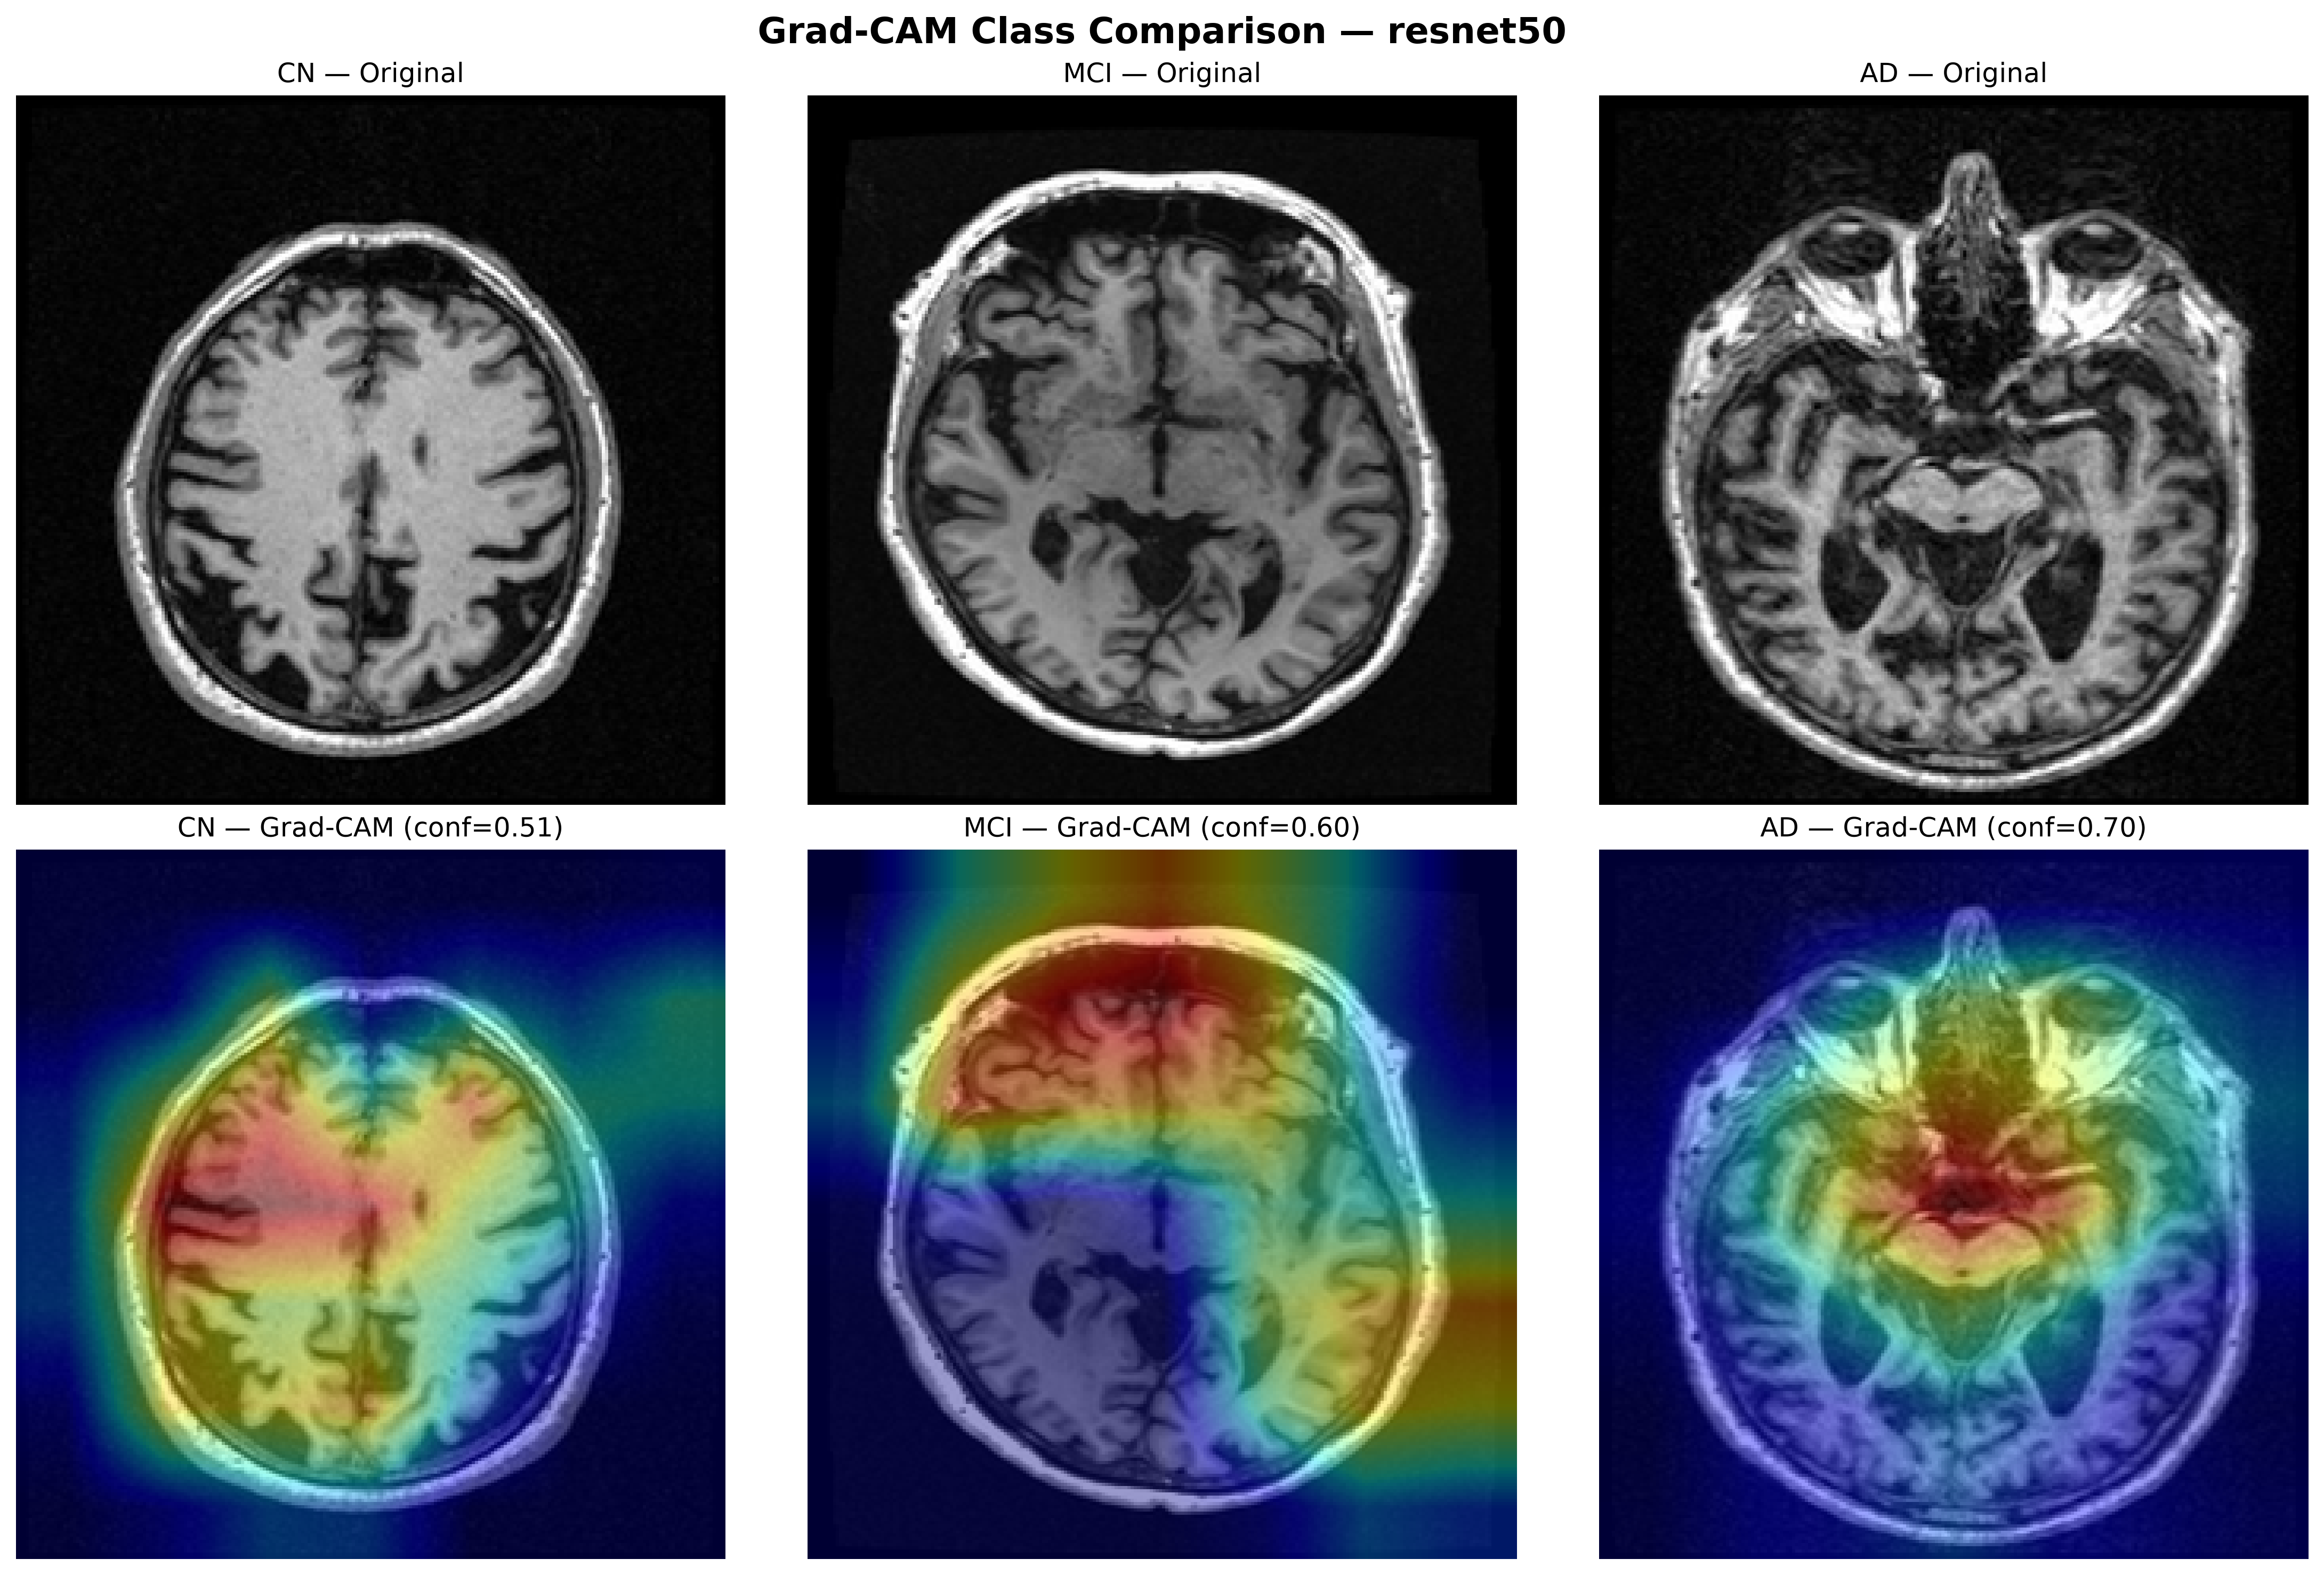
\includegraphics[width=\columnwidth]{resnet50_gradcam_comparison.png}
  \caption{Grad-CAM class-comparison heatmaps for the non-DP
    centralised ResNet50 reference model across CN, MCI, and AD
    categories (fold~0, held-out test slices).  Shown as the reference
    point for the DP-similarity analysis of Section~\ref{sec:xai_dp};
    not offered as evidence of clinical biomarker alignment given this
    model's near-chance accuracy.}
  \label{fig:gradcam}
\end{figure}

\begin{figure}[t]
  \centering
  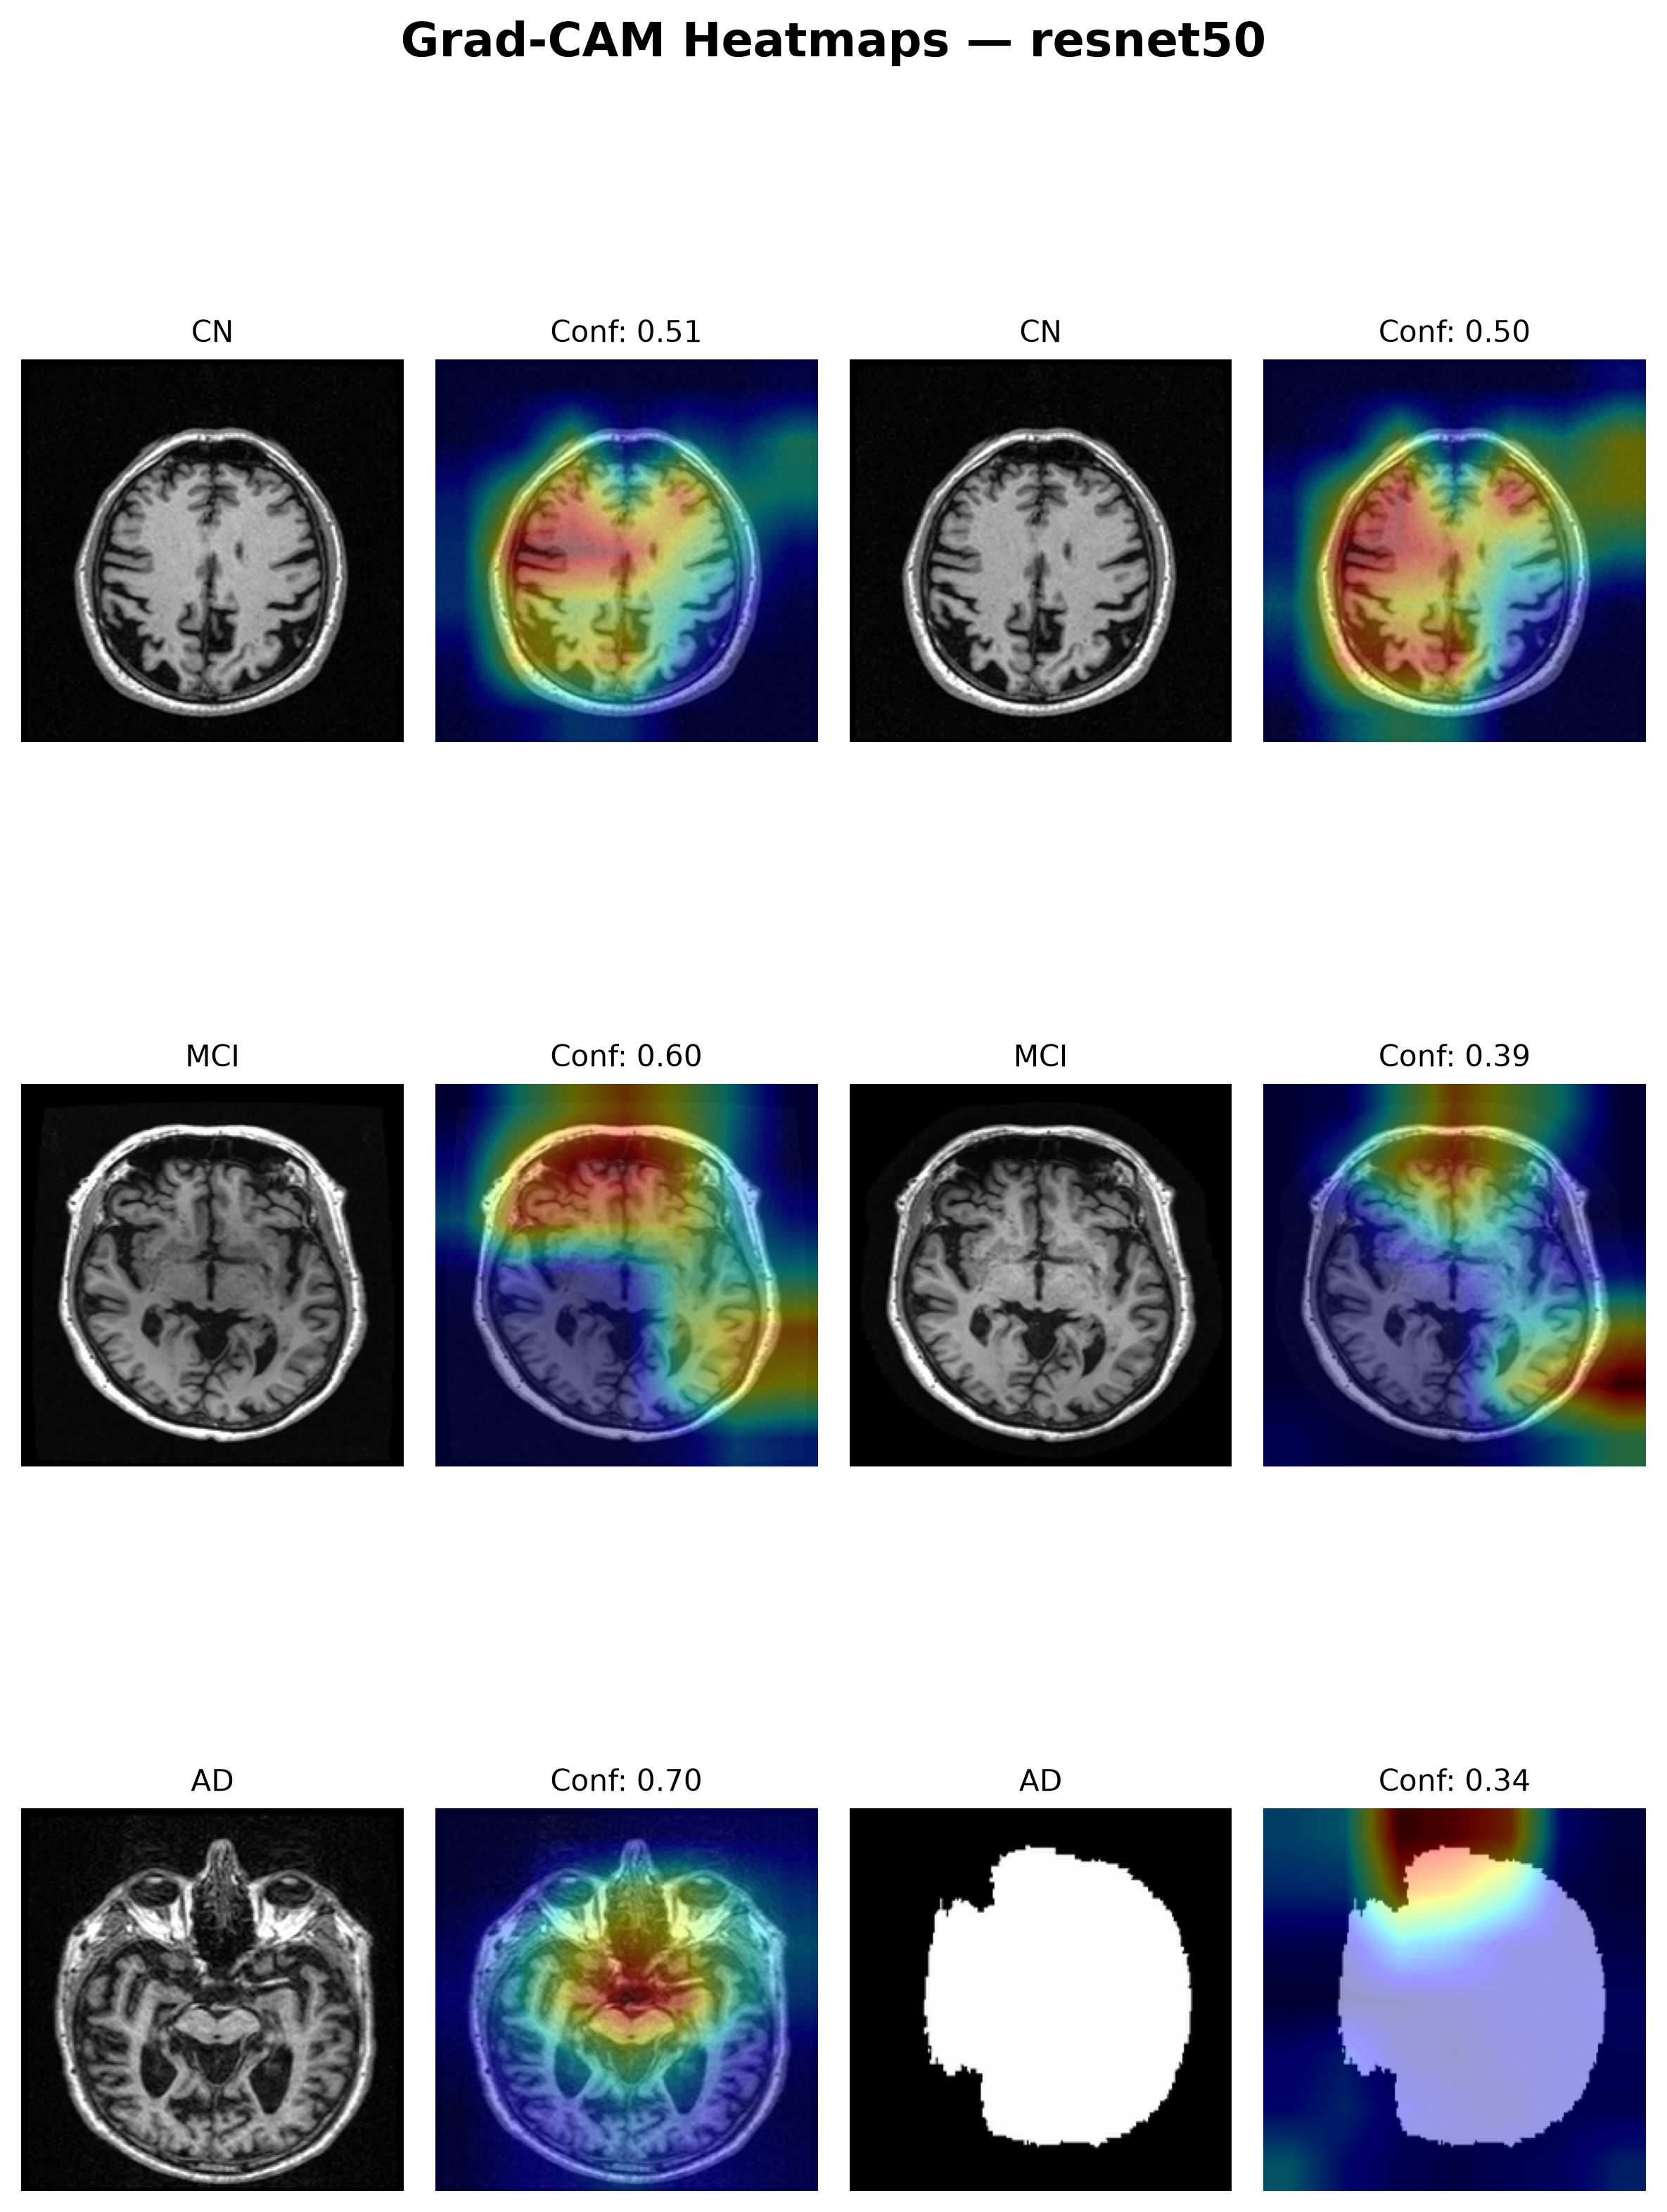
\includegraphics[width=\columnwidth]{resnet50_gradcam_grid.png}
  \caption{Grad-CAM heatmap grid, multiple held-out test subjects per
    diagnostic category, non-DP centralised ResNet50 reference model
    (fold~0).}
  \label{fig:gradcam_grid}
\end{figure}

\subsection{Explanation Degradation Under Differential Privacy}
\label{sec:xai_dp}

The preceding figures show Grad-CAM/SHAP for the non-DP ResNet50
reference model.  A natural question the utility and MIA results
(Sections~\ref{sec:privacy_utility_results},~\ref{sec:mia_results}) do
not answer is whether DP training changes \emph{what the model is
looking at}, independent of whether it changes \emph{how well it
performs}.  We compute Grad-CAM and SHAP on the same held-out test
slices (fold~0) for every DP checkpoint and its matched non-DP
reference (centralised or FedAvg, as appropriate), and summarise
heatmap similarity via SSIM, Spearman rank correlation, and
Dice-at-top-20\%.

\begin{table}[t]
  \centering
  \caption{Grad-CAM Similarity vs.\ Matched Non-DP Reference, fold~0}
  \label{tab:xai_similarity}
  \renewcommand{\arraystretch}{1.15}
  \setlength{\tabcolsep}{2.5pt}
  \footnotesize
  \begin{tabular}{llccc}
    \toprule
    \textbf{Setting} & $\boldsymbol{\varepsilon}$ & \textbf{SSIM} & \textbf{Spearman} & \textbf{Dice@20\%} \\
    \midrule
    \multirow{3}{*}{Centralised, head-only DP}
      & 2  & 0.250 & 0.038  & 0.246 \\
      & 5  & 0.208 & $-$0.014 & 0.200 \\
      & 10 & 0.328 & 0.032  & 0.247 \\
    \multirow{3}{*}{Centralised, full-network DP}
      & 2  & 0.340 & 0.126  & 0.252 \\
      & 5  & 0.304 & 0.072  & 0.314 \\
      & 10 & 0.280 & 0.061  & 0.251 \\
    \multirow{3}{*}{FedAvg, head-only DP}
      & 2  & 0.244 & $-$0.026 & 0.200 \\
      & 5  & 0.269 & $-$0.038 & 0.201 \\
      & 10 & 0.245 & $-$0.005 & 0.207 \\
    FedAvg, full-network DP & 5 & 0.199 & $-$0.244 & 0.133 \\
    \bottomrule
  \end{tabular}
\end{table}

SSIM against the non-DP reference ranges only $0.20$--$0.34$ across
every DP configuration---far from the near-1.0 similarity that would
indicate DP leaves explanations essentially unchanged---and Spearman
rank correlation is frequently at or below zero, meaning the DP
model's most- and least-important pixels are, at best, unrelated to
the non-DP model's, and at worst inversely related (most starkly for
FedAvg full-network DP, Spearman~$-0.244$).  This holds \emph{even for
DP configurations whose accuracy is close to the non-DP reference}
(e.g., centralised head-only DP at $\varepsilon{=}10$: 31.4\% vs.\
30.1\% accuracy, yet Grad-CAM SSIM only 0.328): two models can agree
on the diagnosis while disagreeing substantially on the spatial
evidence for it.  For a clinical deployment where the heatmap itself
is presented to a radiologist as supporting evidence, this is a risk
that accuracy or even MIA metrics alone would not surface, and one we
had no way to observe before running this comparison.  We do not find
a consistent monotonic trend across $\varepsilon$ (mirroring
Section~\ref{sec:privacy_utility_results}'s utility results), and
report the pattern rather than fit a narrative to it.
Fig.~\ref{fig:tradeoff}(c) plots SSIM against $\varepsilon$ for the
three configurations swept across all three $\varepsilon$ values.

\subsection{SHAP Feature Attribution}

SHAP analysis using GradientExplainer with 20~background samples and
50~held-out test slices (fold~0, non-DP centralised ResNet50)
provides global feature importance maps.  Fig.~\ref{fig:shap_summary}
shows the mean absolute SHAP values aggregated spatially, and
Fig.~\ref{fig:shap_examples} presents per-sample SHAP overlays.  As
with the Grad-CAM figures above, we present these as descriptive
output of the pipeline's explainability module rather than as
validated clinical findings, for the same reason: a model at
near-chance held-out accuracy is not a sound basis for biomarker
claims, however plausible individual heatmaps may look in isolation.
This is precisely the caution Section~\ref{sec:leakage}'s leakage
audit is meant to instil---a slice-level-evaluated version of this
same model would have reported 91\% accuracy and made the biomarker
claim far more tempting to accept at face value.

\begin{figure}[t]
  \centering
  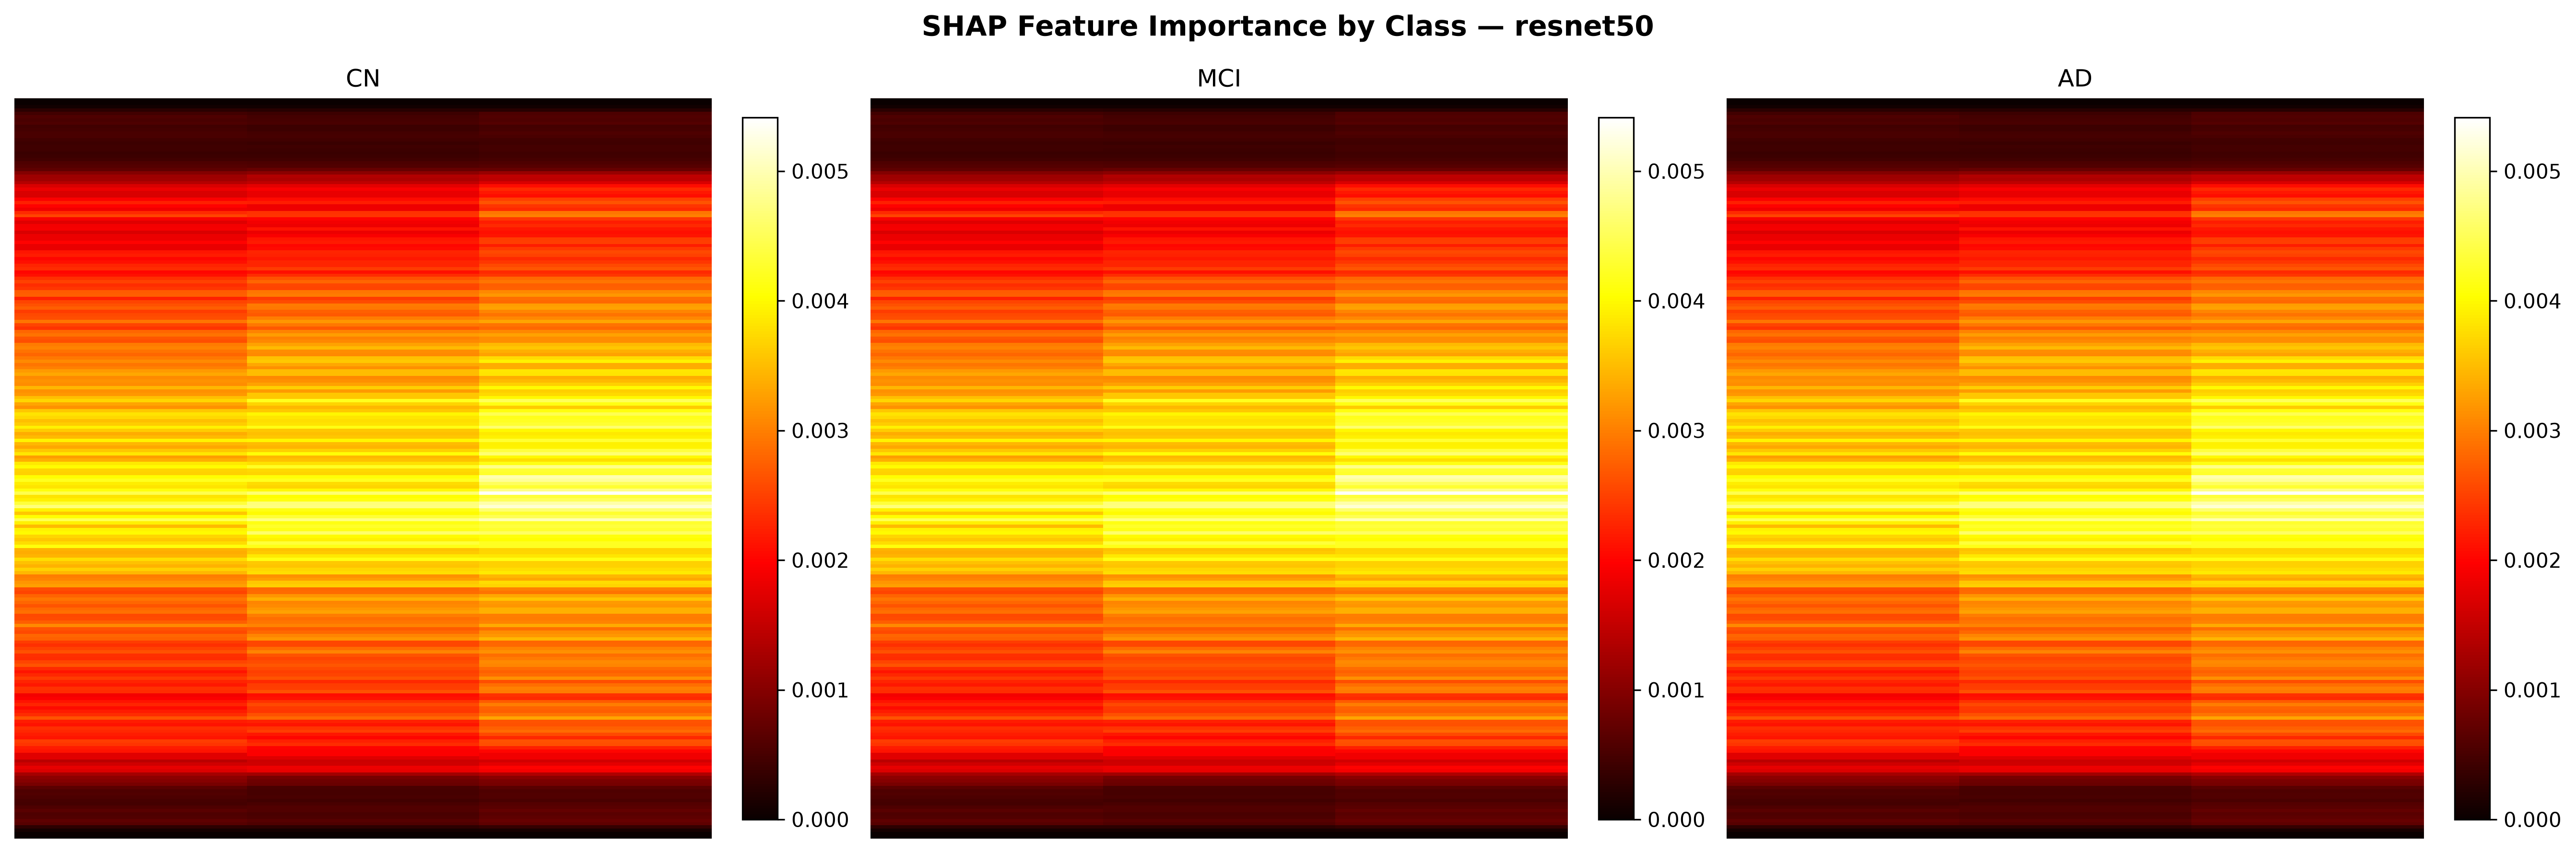
\includegraphics[width=\columnwidth]{resnet50_shap_summary.png}
  \caption{SHAP summary heatmap, mean absolute feature importance,
    non-DP centralised ResNet50 reference model (fold~0).}
  \label{fig:shap_summary}
\end{figure}

\begin{figure}[t]
  \centering
  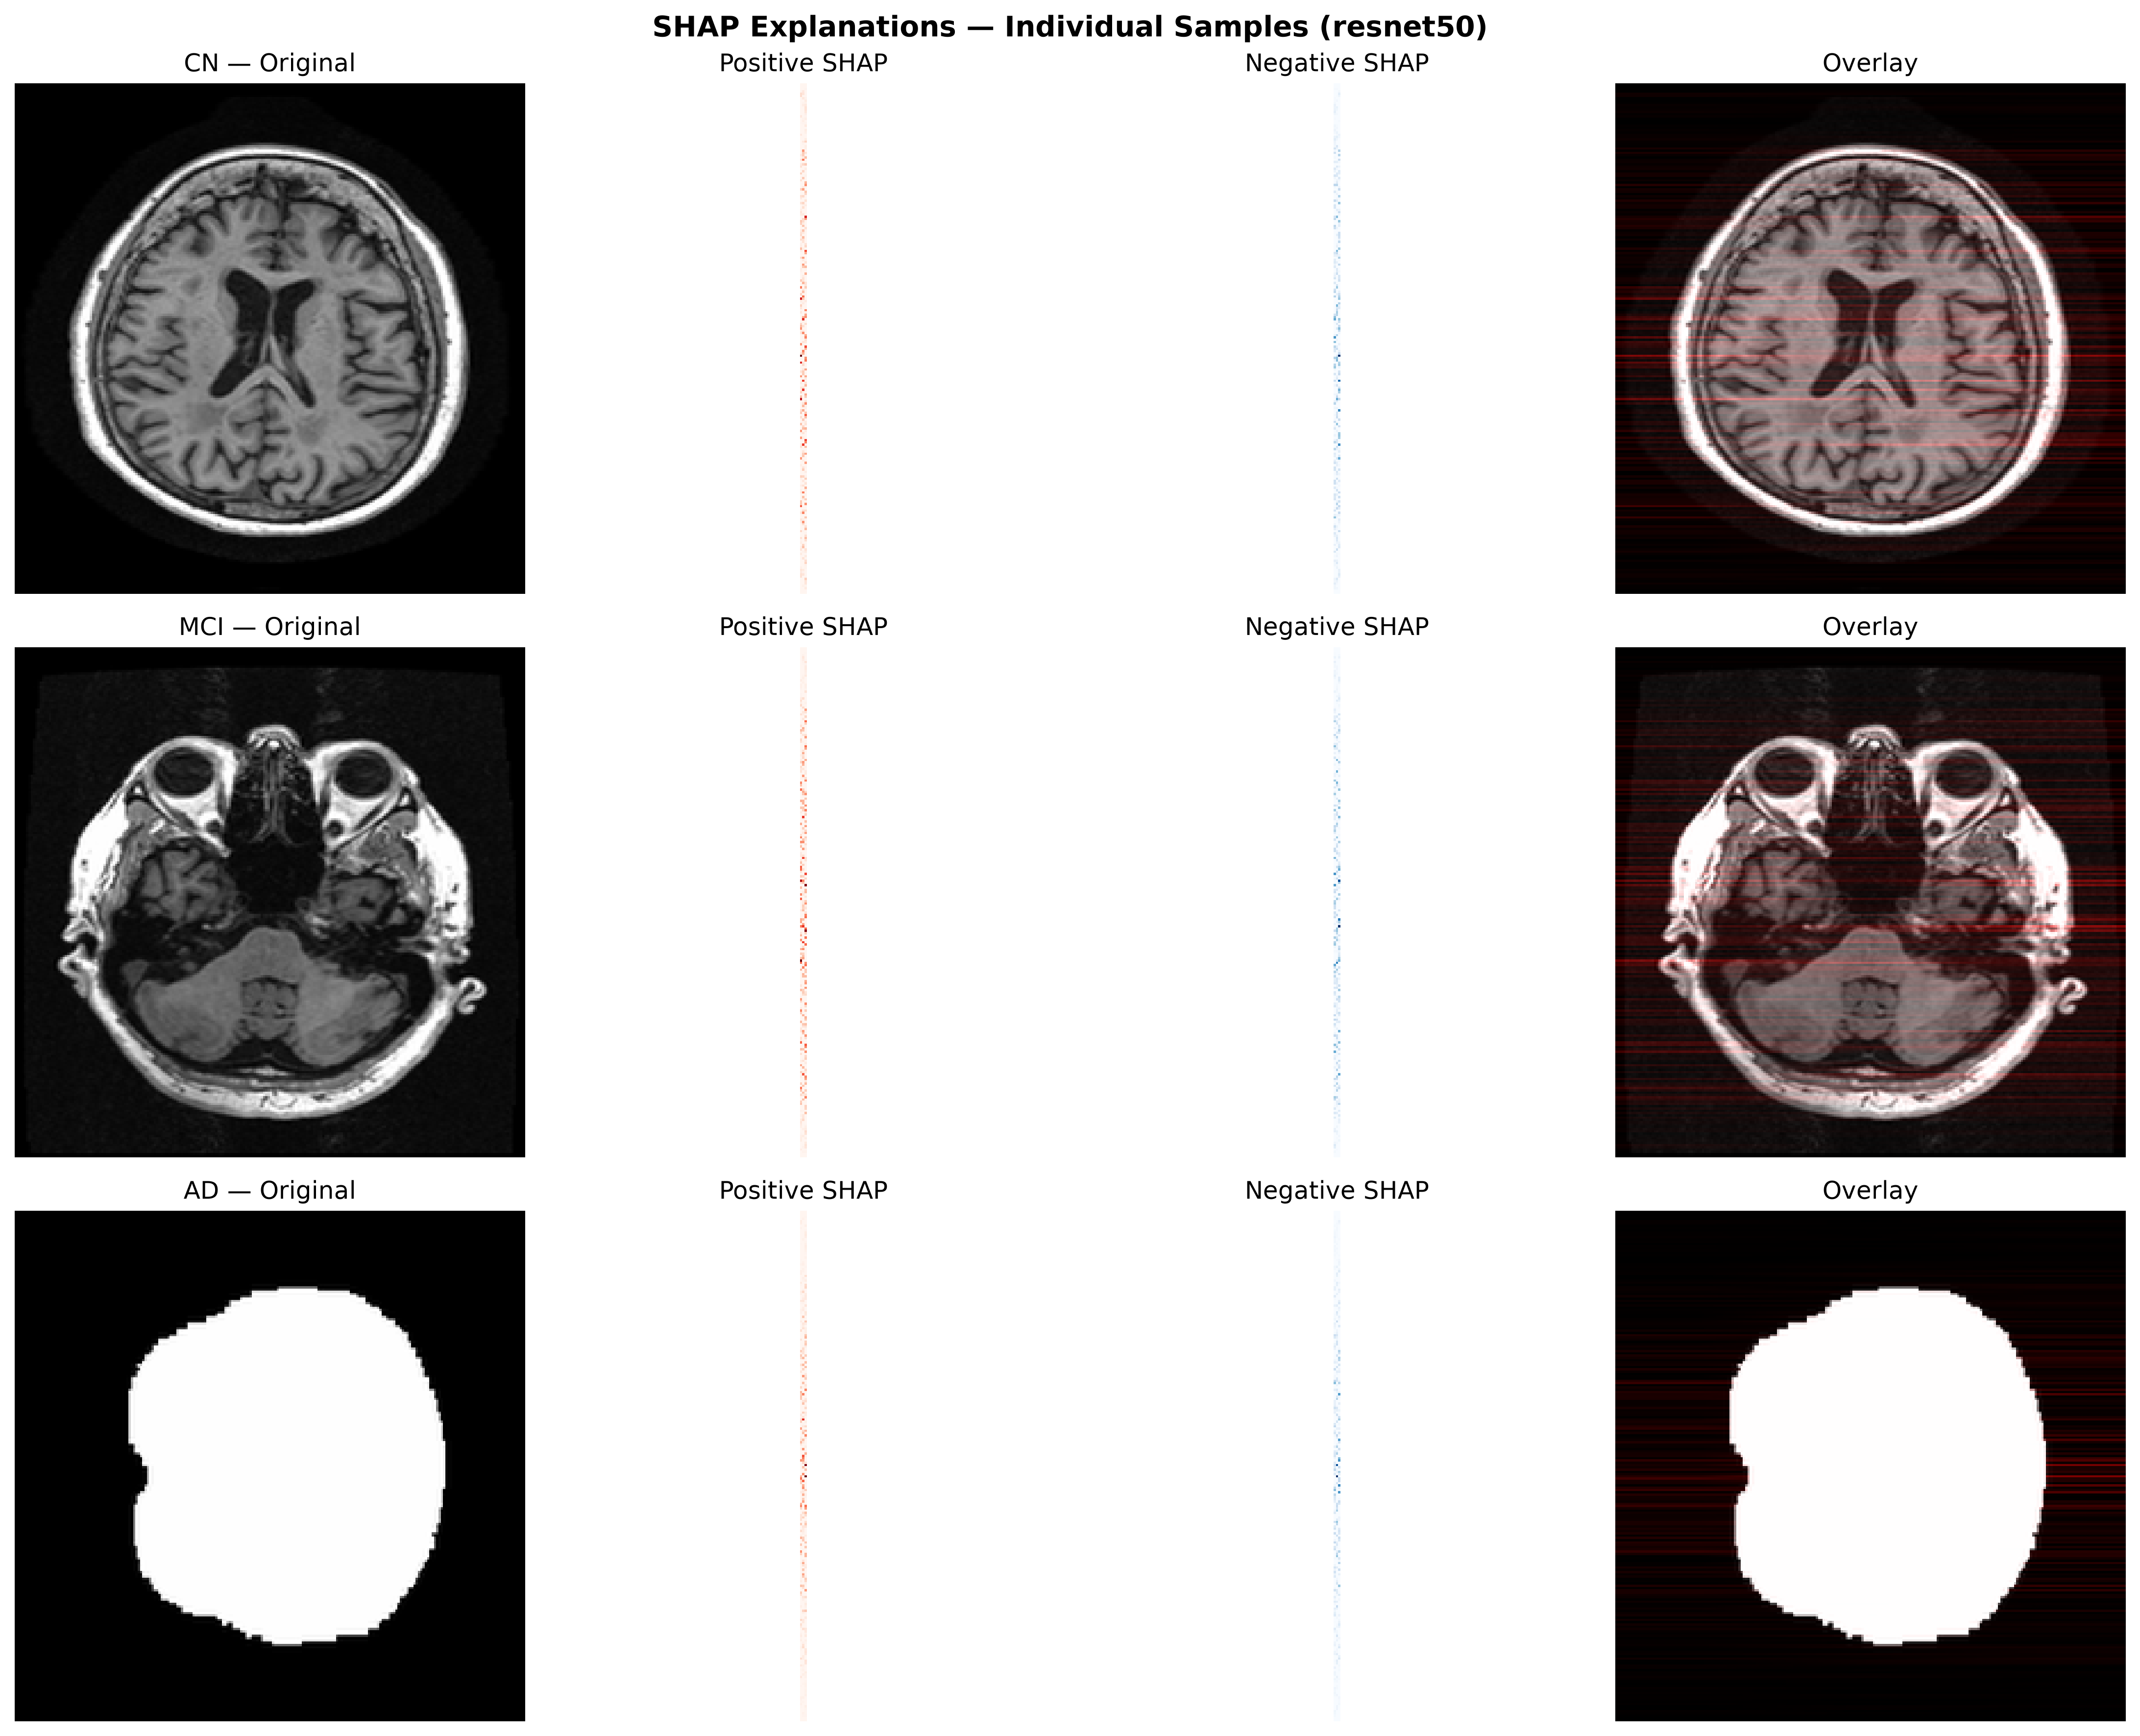
\includegraphics[width=\columnwidth]{resnet50_shap_examples.png}
  \caption{Per-sample SHAP overlays for representative CN, MCI, and AD
    held-out test slices, non-DP centralised ResNet50 reference model
    (fold~0).}
  \label{fig:shap_examples}
\end{figure}

\subsection{Clinical Utility}

The dual-layer explainability design (Grad-CAM for spatial localisation
and SHAP for global attribution) provides complementary clinical
perspectives.  Radiologists can use Grad-CAM heatmaps for scan-level
inspection; neurologists can leverage SHAP summaries for population-level
insights.  This interpretability layer is essential for regulatory
approval and clinical trust in AI-assisted diagnosis, as demonstrated
by Mastoi et al.~\cite{mastoi2025}.

% ============================================================
\section{Verification and Reproducibility}
\label{sec:verification}
% ============================================================

The central claim of this paper is a negative one about evaluation
protocol, so the protocol itself has to be checkable rather than
asserted.  Three mechanisms do that.

\subsection{Automated Verification of the Split Property}

The subject-disjointness property of Section~\ref{sec:dataset_honest}
is asserted programmatically, not by inspection.  A verification suite
loads the shipped splits file and, for each of the five folds, checks
that no subject appears in more than one of train, validation and
test, that no array index is reachable from two partitions, and that
the union of the three partitions is exactly the 299-subject cohort.
The same suite validates every recorded results file against a schema:
required metrics present, all metrics within $[0, 1]$, and for every
private run an achieved $\varepsilon$ within 15\% of its target.  That
last check surfaced a real detail worth stating: the accountant's
noise-multiplier search overshoots the target budget by up to $0.2\%$,
so the guarantee we report is the \emph{achieved} $\varepsilon$ rather
than the requested one.

\subsection{Machine-Generated Tables}

Every numeric table in this paper is written into marker-delimited
blocks in the \LaTeX{} source by a generator that reads the aggregated
results JSON directly.  No result in a table is typed by hand, so a
table cannot drift from the experiment behind it.  A separate checker
guards the prose, where numbers are still written by a person: it
traces every percentage in the text to a recorded result---a pooled
condition mean, an individual run, or an ablation cell---and fails on
anything it cannot account for, with a small allow-list of documented
non-results such as the chance rate and the superseded slice-level
figures this paper corrects.  That checker found one genuine defect
during preparation: a sentence citing the 32-subject accuracy beside a
table that by then held the 299-subject result.

\subsection{Test Suite and Continuous Integration}

The pure-logic modules of the pipeline---subject-level splitting,
Dirichlet client partitioning, model construction, the FedAvg and
DP-FedAvg aggregation arithmetic, results aggregation, and the
statistical analysis---are covered by a test suite held at 100\%
statement and branch coverage on that measured scope, enforced in
continuous integration.  The CUDA training loops are excluded from
measurement rather than mocked: a mock of a training loop tests the
mock.  The exclusions and the reason for each are documented alongside
the suite.  Tests run on synthetic fixtures and need no ADNI access,
so the pipeline is verifiable by a reader who cannot obtain the data.

Continuous integration runs five sequential stages on every push:
build, test, lint, package, and deployment of the interactive
demonstration.  A secret-scanning step guards the repository, and the
coverage gate fails the build rather than reporting a lower number.

% ============================================================

\section{Limitations}
\label{sec:limitations}
% ============================================================

\textbf{Cohort Size.}\;This is the paper's central limitation, not a
minor caveat: our ADNI cohort contains only 32~unique subjects.  Every
subject-level result in this paper should be read as a
small-cohort feasibility and methodology study, not as evidence of
clinical-grade diagnostic accuracy---held-out accuracy across every
architecture and training regime we evaluated (Sections~\ref{sec:results}--\ref{sec:privacy})
sits within a few points of three-class chance (33.3\%). We disclose
this prominently precisely because our own earlier slice-level
evaluation of the identical models and data did not, and reported
91--97\% accuracy instead (Section~\ref{sec:leakage}).  No claim in
this paper should be read as evidence that the described models are
ready, or close to ready, for clinical use.

\textbf{Slice-Level DP Unit.}\;Our DP accountant bounds sensitivity at
the slice level, not the subject level (Section~\ref{sec:privacy}).  A
subject contributing multiple scans receives a looser effective
per-subject privacy guarantee than the reported per-slice
$\varepsilon$; a rigorous per-subject guarantee would require
group-level DP-SGD (clipping and accounting per subject, not per
slice), which we did not implement.

\textbf{Simulated Environment.}\;Validation on a simulated multi-client
setup does not capture the full complexity of real distributed hospital
infrastructure (network latency, heterogeneous hardware, asynchronous
training).

\textbf{Non-IID Approximation.}\;Dirichlet-sampled splits approximate
but do not fully replicate real hospital demographic heterogeneity
influenced by referral patterns, scanner models, and clinical protocols;
at our cohort size, some Dirichlet draws additionally required a
retry loop to avoid assigning a client zero training subjects
(Section~\ref{sec:fl_config}).

\textbf{No Clean Privacy--Utility Trend.}\;We did not observe a
consistent monotonic accuracy-vs-$\varepsilon$ relationship
(Section~\ref{sec:privacy_utility_results}); with only 5--7
folds/seeds per configuration and $\sim$22--26 training subjects each,
subject-composition variance dominates any systematic DP effect at
this scale.  Larger cohorts are needed to isolate the trend cleanly.

\textbf{Compute Constraints Shaped Coverage.}\;Full-network DP-FL
(Table~\ref{tab:dp_results}) is reported at a single $\varepsilon$ as
a feasibility check rather than a full sweep, and FedAvg VGG19
(Table~\ref{tab:fedavg}) at fold~0 only, because Opacus's per-sample
gradient memory cost was prohibitive for a full matrix on our 4\,GB
GPU within a practical time budget; this reflects hardware
constraints, not a judgement that these configurations are
uninteresting.

\textbf{Dataset Scope.}\;ADNI~\cite{adni} represents a specific
demographic and geographical distribution; generalisability to non-ADNI
populations, or to larger ADNI subsets, requires further validation
and is exactly the direction this paper's corrected pipeline is built
to support.

\textbf{GPU Memory Constraints.}\;VGG19's 139.6M parameters and
Opacus's per-sample gradient hooks required careful batch-size
management on our 4\,GB GPU, favouring ResNet50 as the primary
architecture for the DP, MIA, and explainability experiments.

% ============================================================
\section{Future Work}
\label{sec:future}
% ============================================================

\textbf{Cohort Expansion.}\;The single highest-priority next step is
re-running this exact pipeline on substantially more ADNI subjects
(target: 50+ unique subjects per class).  Because every result in
this paper is subject-level and the pipeline is manifest-driven
(Section~\ref{sec:dataset_honest}), this requires no methodological
change---only more data---and would let the privacy--utility and
privacy--explainability trends of Sections~\ref{sec:privacy_utility_results}--\ref{sec:xai_dp}
be measured with enough subjects to separate a systematic DP effect
from small-cohort composition noise.

\textbf{Adaptive DP Budget Allocation.}\;Per-round adaptive noise
scheduling that reduces DP noise as federated convergence is detected,
improving late-training accuracy without increasing total privacy
cost~\cite{abadi2016}.

\textbf{Personalised Federated Learning.}\;Per-FedPer and MAML-based
personalisation to address non-IID heterogeneity while preserving global
aggregation privacy guarantees.

\textbf{Multimodal Fusion.}\;Joint processing of MRI scans and tabular
clinical variables (MMSE scores, genetic biomarkers) in a federated
multimodal architecture following Pan et al.~\cite{pan2025}.

\textbf{Federated XAI Enhancements.}\;Federated SHAP approximations
aggregating locally computed Shapley values without exposing client data
distributions, enabling globally representative explanations.

\textbf{Real-World Deployment.}\;Piloting on real distributed hospital
infrastructure with asynchronous aggregation and dropout-tolerant
variants.

\textbf{Longitudinal Prediction.}\;Extension to MCI-to-AD progression
prediction via federated LSTM or transformer architectures operating on
longitudinal imaging sequences.

% ============================================================
\section{Conclusion}
\label{sec:conclusion}
% ============================================================

This paper presented PPXFL, a Privacy-Preserving and Explainable
Federated Learning framework for Alzheimer's Disease detection from
MRI data---and, more centrally, a corrected re-evaluation of that same
framework after discovering that our initial slice-level evaluation
protocol had leaked subject identity across train/validation/test
splits.  Our key findings are:

\begin{enumerate}
\item \textbf{Slice-level evaluation severely inflates reported
  accuracy.}\;On identical models and data, subject-disjoint
  evaluation collapses accuracy from a reported 91--97\% to a genuine
  19--36\%---within a few points of three-class chance (33.3\%) for a
  32-subject cohort.  We release the corrected splits and full result
  set so this comparison is independently verifiable
  (Section~\ref{sec:leakage}).

\item \textbf{Differential privacy virtually eliminates membership
  inference at negligible marginal utility cost.}\;A real shadow-model
  attack shows non-DP models are almost perfectly vulnerable
  (AUC~0.96--0.99); every DP configuration we tested
  ($\varepsilon\in\{2,5,10\}$, head-only or full-network, centralised
  or federated) collapses this to near-chance
  (AUC~0.42--0.69)~\cite{opacus,shokri2017,yeom2018}, while accuracy
  changes only modestly relative to the already utility-constrained
  non-DP baseline (Sections~\ref{sec:privacy_utility_results}--\ref{sec:mia_results}).

\item \textbf{Head-only DP fine-tuning is a practical utility-rescue
  recipe.}\;Freezing the backbone and applying DP-SGD only to the
  classification head consistently retains more accuracy than
  full-network DP at every $\varepsilon$ tested, without sacrificing
  MIA resistance.

\item \textbf{Differential privacy changes what a model explains, not
  only how well it performs.}\;Grad-CAM similarity between DP and
  non-DP models is low (SSIM~0.20--0.34) even when their accuracy is
  comparable, indicating that DP training relocates the model's
  attention in ways that raw accuracy or MIA metrics do not surface
  (Section~\ref{sec:xai_dp}).

\item \textbf{Severe non-IID heterogeneity remains a genuine failure
  mode even at small scale.}\;Ablations show accuracy dropping to
  21.0\% under severe non-IID partitioning ($\alpha{=}0.1$), the
  clearest degradation we observe outside the DP experiments
  themselves.
\end{enumerate}

We present PPXFL's corrected pipeline and results as a methodological
contribution as much as a system contribution: a concrete, reproducible
illustration of why subject-level evaluation is not optional in
small-cohort medical imaging FL research, alongside the first
systematic privacy--utility--explainability characterisation we are
aware of for DP-SGD on Alzheimer's MRI classification.  Future work
will prioritise cohort expansion to disentangle systematic DP effects
from small-cohort noise, followed by adaptive DP scheduling,
personalised FL, and real-world multi-institutional deployment.

% ============================================================
\section*{Acknowledgement}
% ============================================================

The authors thank Prof.\ Agha Alfi Mirza for project guidance and the
Department of Computer Science \& Engineering, PES University, Bangalore,
for institutional support.  Data collection and sharing were funded by the
Alzheimer's Disease Neuroimaging Initiative~(ADNI)
(NIH Grant U01~AG024904).  The investigators at ADNI contributed to the
design and implementation of ADNI and/or provided data, but did not
participate in the analysis or writing of this report.

% ============================================================
\balance
\begin{thebibliography}{16}

\bibitem{mitrovska2024}
A.~Mitrovska, P.~Safari, K.~Ritter, B.~Shariati, and J.~K.~Fischer,
``Secure federated learning for Alzheimer's disease detection,''
\textit{Front.\ Aging Neurosci.}, vol.~16, p.~1324032, Mar.~2024.

\bibitem{mastoi2025}
Q.~Mastoi, S.~Latif, S.~Brohi, J.~Ahmad, A.~Alqhatani,
M.~S.~Alshehri, A.~Al~Mazroa, and R.~Ullah,
``Explainable AI in medical imaging: An interpretable and collaborative
federated learning model for brain tumor classification,''
\textit{Front.\ Oncol.}, vol.~15, p.~1535478, Jan.~2025.

\bibitem{pan2025}
J.~Pan, Z.~Fan, G.~E.~Smith, Y.~Guo, J.~Bian, and J.~Xu,
``Federated learning with multi-cohort real-world data for predicting
the progression from mild cognitive impairment to Alzheimer's disease,''
\textit{Alzheimer's Dement.}, vol.~21, no.~4, p.~e70128, 2025.

\bibitem{privacy2024}
G.~Kaissis, M.~Makowski, D.~R\"{u}ckert, and R.~Braren,
``Privacy-preserving federated learning and uncertainty quantification
in medical imaging,''
\textit{Radiol.\ Artif.\ Intell.}, p.~240637, 2024.

\bibitem{evolutionary2025}
N.~Basnin, T.~Mahmud, R.~U.~Islam, and K.~Andersson,
``An evolutionary federated learning approach to diagnose Alzheimer's
disease under uncertainty,''
\textit{Diagnostics}, vol.~15, no.~1, p.~80, 2025.

\bibitem{mcmahan2017}
H.~B.~McMahan, E.~Moore, D.~Ramage, S.~Hampson, and B.~A.~y~Arcas,
``Communication-efficient learning of deep networks from decentralized
data,''
in \textit{Proc.\ 20th Int.\ Conf.\ Artif.\ Intell.\ Statist.\
(AISTATS)}, 2017, pp.~1273--1282.

\bibitem{bonawitz2017}
K.~Bonawitz et al.,
``Practical secure aggregation for privacy-preserving machine learning,''
in \textit{Proc.\ ACM SIGSAC Conf.\ Comput.\ Commun.\ Secur.\ (CCS)},
2017, pp.~1175--1191.

\bibitem{dwork2014}
C.~Dwork and A.~Roth,
``The algorithmic foundations of differential privacy,''
\textit{Found.\ Trends Theor.\ Comput.\ Sci.}, vol.~9, no.~3--4,
pp.~211--407, 2014.

\bibitem{abadi2016}
M.~Abadi et al.,
``Deep learning with differential privacy,''
in \textit{Proc.\ ACM SIGSAC Conf.\ Comput.\ Commun.\ Secur.\ (CCS)},
2016, pp.~308--318.

\bibitem{gradcam}
R.~R.~Selvaraju, M.~Cogswell, A.~Das, R.~Vedantam, D.~Parikh, and
D.~Batra,
``Grad-CAM: Visual explanations from deep networks via gradient-based
localization,''
in \textit{Proc.\ IEEE Int.\ Conf.\ Comput.\ Vis.\ (ICCV)}, 2017,
pp.~618--626.

\bibitem{shap}
S.~M.~Lundberg and S.-I.~Lee,
``A unified approach to interpreting model predictions,''
in \textit{Adv.\ Neural Inf.\ Process.\ Syst.\ (NeurIPS)}, 2017,
pp.~4765--4774.

\bibitem{vgg19}
K.~Simonyan and A.~Zisserman,
``Very deep convolutional networks for large-scale image recognition,''
in \textit{Proc.\ Int.\ Conf.\ Learn.\ Represent.\ (ICLR)}, 2015.

\bibitem{resnet50}
K.~He, X.~Zhang, S.~Ren, and J.~Sun,
``Deep residual learning for image recognition,''
in \textit{Proc.\ IEEE Conf.\ Comput.\ Vis.\ Pattern Recognit.\
(CVPR)}, 2016, pp.~770--778.

\bibitem{opacus}
A.~Yousefpour et al.,
``Opacus: User-friendly differential privacy library in PyTorch,''
\textit{arXiv preprint arXiv:2109.12298}, 2021.

\bibitem{adni}
R.~C.~Petersen et al.,
``Alzheimer's Disease Neuroimaging Initiative (ADNI): Clinical
characterization,''
\textit{Neurology}, vol.~74, no.~3, pp.~201--209, Jan.~2010.

\bibitem{zhu2019}
L.~Zhu, Z.~Liu, and S.~Han,
``Deep leakage from gradients,''
in \textit{Adv.\ Neural Inf.\ Process.\ Syst.\ (NeurIPS)}, 2019,
pp.~14747--14756.

\bibitem{shokri2017}
R.~Shokri, M.~Stronati, C.~Song, and V.~Shmatikov,
``Membership inference attacks against machine learning models,''
in \textit{Proc.\ IEEE Symp.\ Secur.\ Priv.\ (SP)}, 2017, pp.~3--18.

\bibitem{yeom2018}
S.~Yeom, I.~Giacomelli, M.~Fredrikson, and S.~Jha,
``Privacy risk in machine learning: Analyzing the connection to
overfitting,''
in \textit{Proc.\ IEEE 31st Comput.\ Secur.\ Found.\ Symp.\ (CSF)},
2018, pp.~268--282.

\bibitem{carlini2022}
N.~Carlini, S.~Chien, M.~Nasr, S.~Song, A.~Terzis, and F.~Tramer,
``Membership inference attacks from first principles,''
in \textit{Proc.\ IEEE Symp.\ Secur.\ Priv.\ (SP)}, 2022, pp.~1897--1914.

\end{thebibliography}

\end{document}
